\documentclass{article}
\usepackage{course_work} % Load your custom package!

\title{
    
\includegraphics[scale=0.2]{Images/cam_logo_bw.png}\\ % Use a relative path!
    \vspace{0.5cm}
    S2: Advanced Statistical Methods
}
\author{Yuchen Mao (ym429)}
\affil{Department of Physics, University of Cambridge}
\date{\today}
\usepackage{array}
\usepackage{siunitx}


\begin{document}

\maketitle
\noindent\textbf{Word count: 2980}
\setpagefooter{2980}{Yuchen Mao} % Set the footer *after* \begin{document}

\tableofcontents
\newpage


% Your content here..
\section{Introduction}
This report details the fine-tuning of the \texttt{Qwen-2.5-0.5B-Instruct} language model for a time-series forecasting task using Low-Rank Adaptation within a defined computational budget. We present the algorithm for FLOPS calculation, discuss LLMTime data preprocessing steps, outline the multi-stage training process involving hyperparameter optimization (learning rate, LoRA rank, context length), and evaluate the model's performance at each stage. The primary goal was to assess the feasibility and effectiveness of adapting a large language model for this specialized, non-linguistic task under resource constraints.

.


\section{Dataset}

\subsection{Dataset and Task} % Added a subsection for clarity

The dataset used in this study represent predator-prey population dynamics, generated with Lotka-Volterra systems. It have 1000 distinct systems, each represented by a time series spanning 100 time steps capturing the population levels of both predator and prey. 

The primary objective of this report is to fine-tune the pre-trained \texttt{Qwen-2.5-0.5B-Instruct} model on this specialized dataset. We aim for the model to learn the underlying temporal dynamics governing the predator-prey interactions and subsequently predict future population levels based on past observations.

To gain qualitative insight into the data, Figure \ref{fig:dataset_examples} visualizes the dynamics of two sampled systems (System 0 and System 16) from the dataset. Both time-series plots (population vs. time) and phase portraits (prey population vs. predator population) are presented.

\begin{figure}[!htbp] % Use positioning options like htbp
    \centering % Center the entire grid

    \begin{subfigure}[b]{0.48\linewidth} % [b] aligns subfigure bottoms
        \centering
        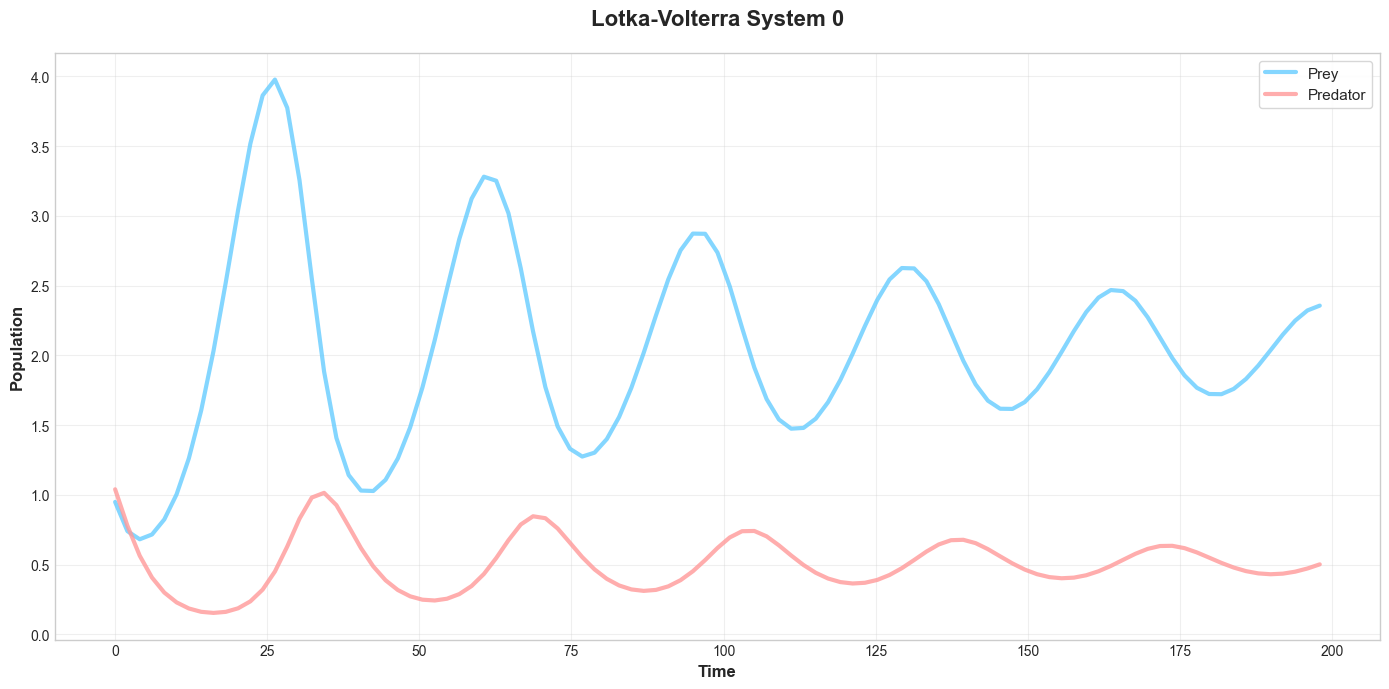
\includegraphics[width=\linewidth]{M2 Course Work//Images/dataset_vis_timeseries_0.png}
        \caption{Time series plot for System 0.}
        \label{fig:ts_0}
    \end{subfigure}
    \hfill % Adds horizontal space between the subfigures
    \begin{subfigure}[b]{0.48\linewidth}
        \centering
        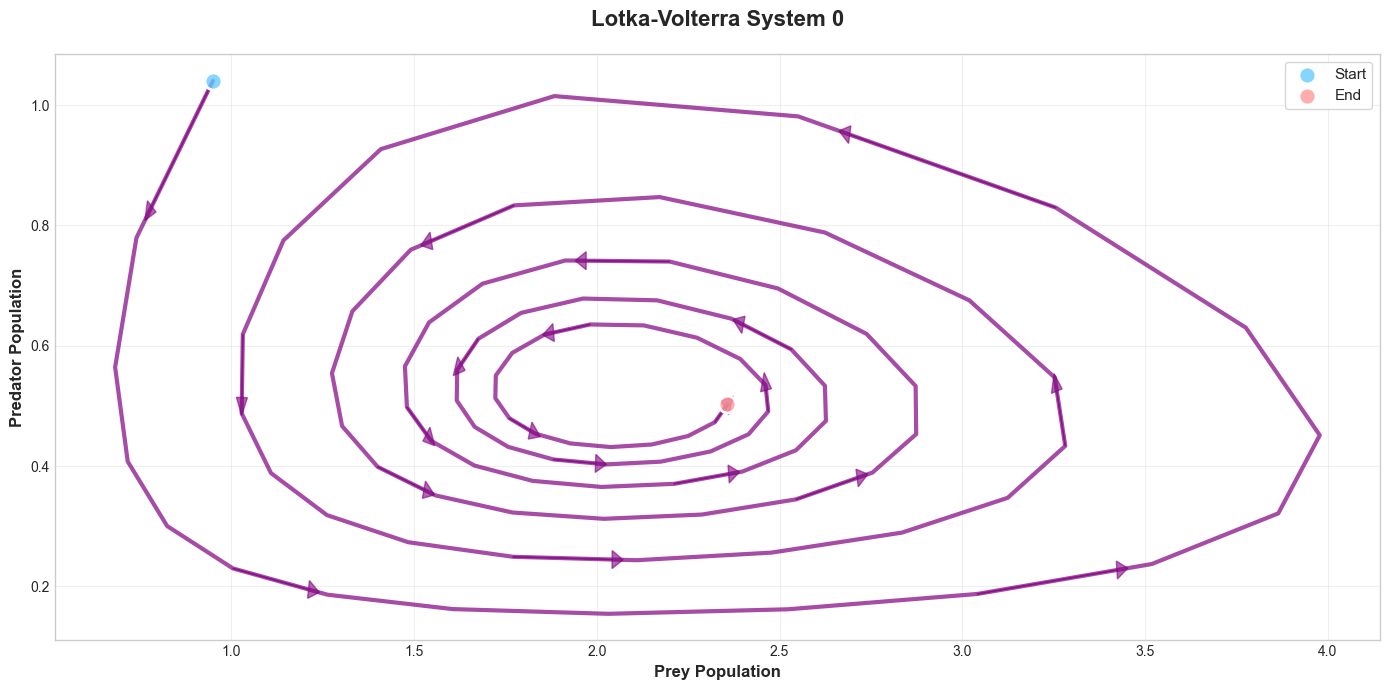
\includegraphics[width=\linewidth]{M2 Course Work//Images/dataset_vis_phase_0.png}
        \caption{Phase portrait for System 0.}
        \label{fig:phase_0}
    \end{subfigure}

    \vspace{0.3cm} % Adds a small vertical space between rows

    \begin{subfigure}[b]{0.48\linewidth}
        \centering
        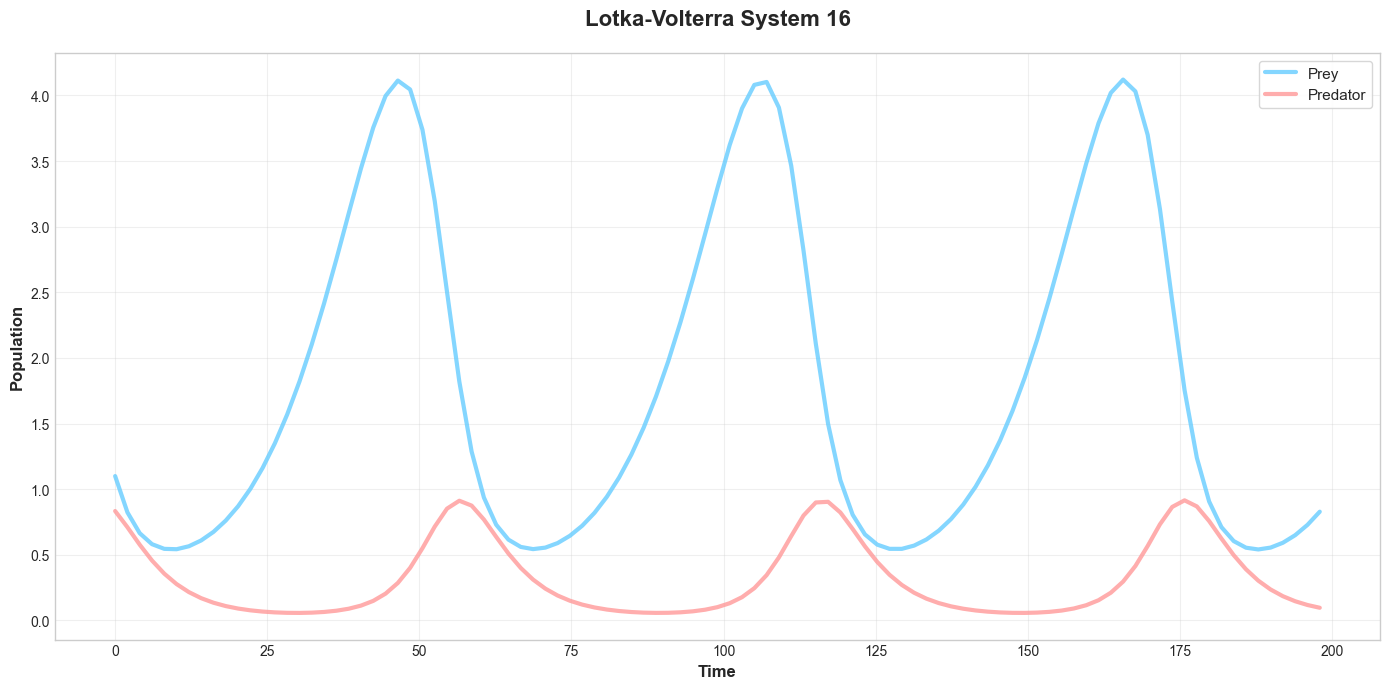
\includegraphics[width=\linewidth]{M2 Course Work//Images/dataset_vis_timeseries_16.png}
        \caption{Time series plot for System 16.}
        \label{fig:ts_16}
    \end{subfigure}
    \hfill % Adds horizontal space
    \begin{subfigure}[b]{0.48\linewidth}
        \centering
        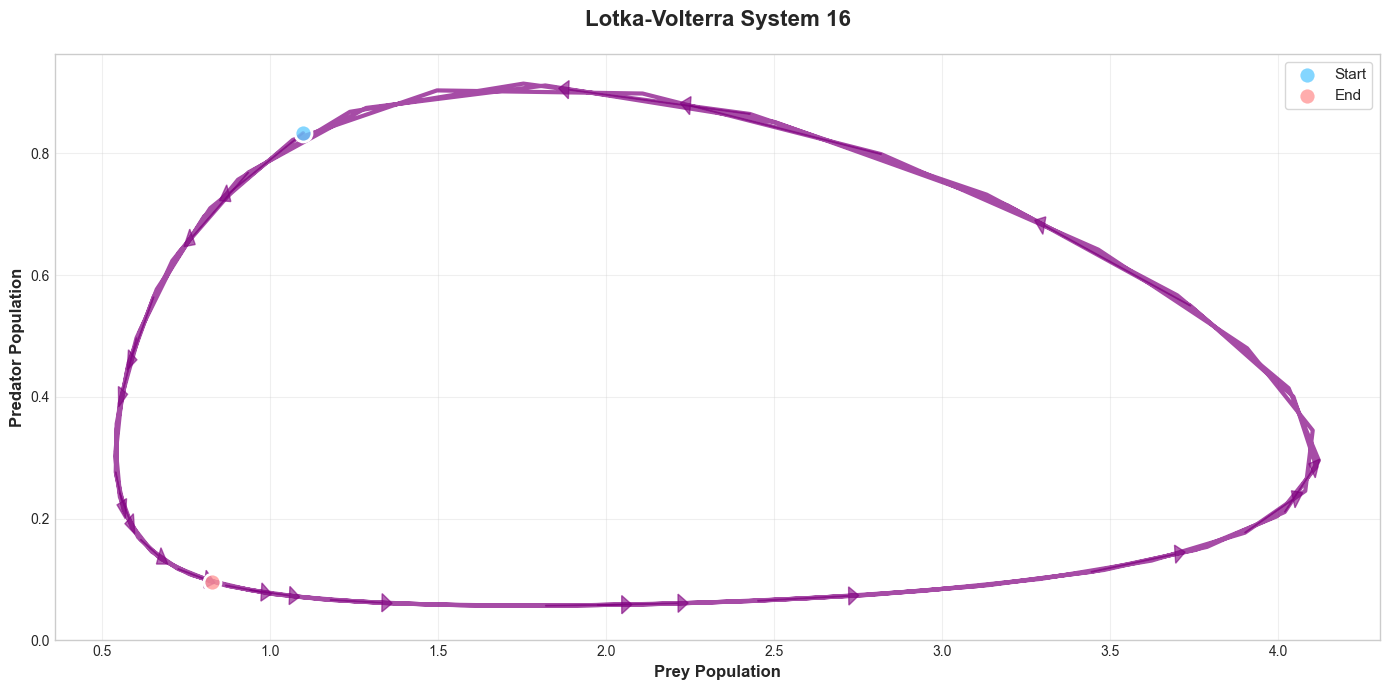
\includegraphics[width=\linewidth]{M2 Course Work//Images/dataset_vis_phase_16.png}
        \caption{Phase portrait for System 16.}
        \label{fig:phase_16}
    \end{subfigure}

    \caption{Visualization of predator-prey dynamics for two example systems (0 and 16) from the dataset. Subfigures (a) and (c) show population levels (Prey in blue, Predator in orange) over 100 time steps. Subfigures (b) and (d) display the corresponding phase plots, illustrating the cyclical relationship between prey and predator populations.}
    \label{fig:dataset_examples} % Unique label for the entire figure
\end{figure}

\section{LLMTime Preprocessor}
\label{sec:preprocessing}

In this study, since we are fine-tuning \texttt{Qwen-2.5-0.5B-instruct}, a language model originally trained on natural language, to perform inference on time-series data. A key challenge in this process is the inefficiency of representing numerical time-series data in a tokenized format suitable for LLMs. For example, the Qwen tokenizer encodes a floating-point number such as $0.12345$ into a verbose sequence of discrete tokens: $[0, ., 1, 2, 3, 4, 5]$. This inefficiency inflates token usage, increasing both training and inference costs. To mitigate this, we adopt the preprocessing method from LLMTime \cite{gruver2024largelanguagemodelszeroshot}. This preprocessing method consist of three steps, scaling, rounding, and formatting, which are depicted in Figure \ref{fig:preprocessing_visual_workflow}. 

% Ensure the image path is correct relative to your .tex file
\begin{figure}[!htbp] % [htbp] suggests placement: here, top, bottom, page
    \centering
    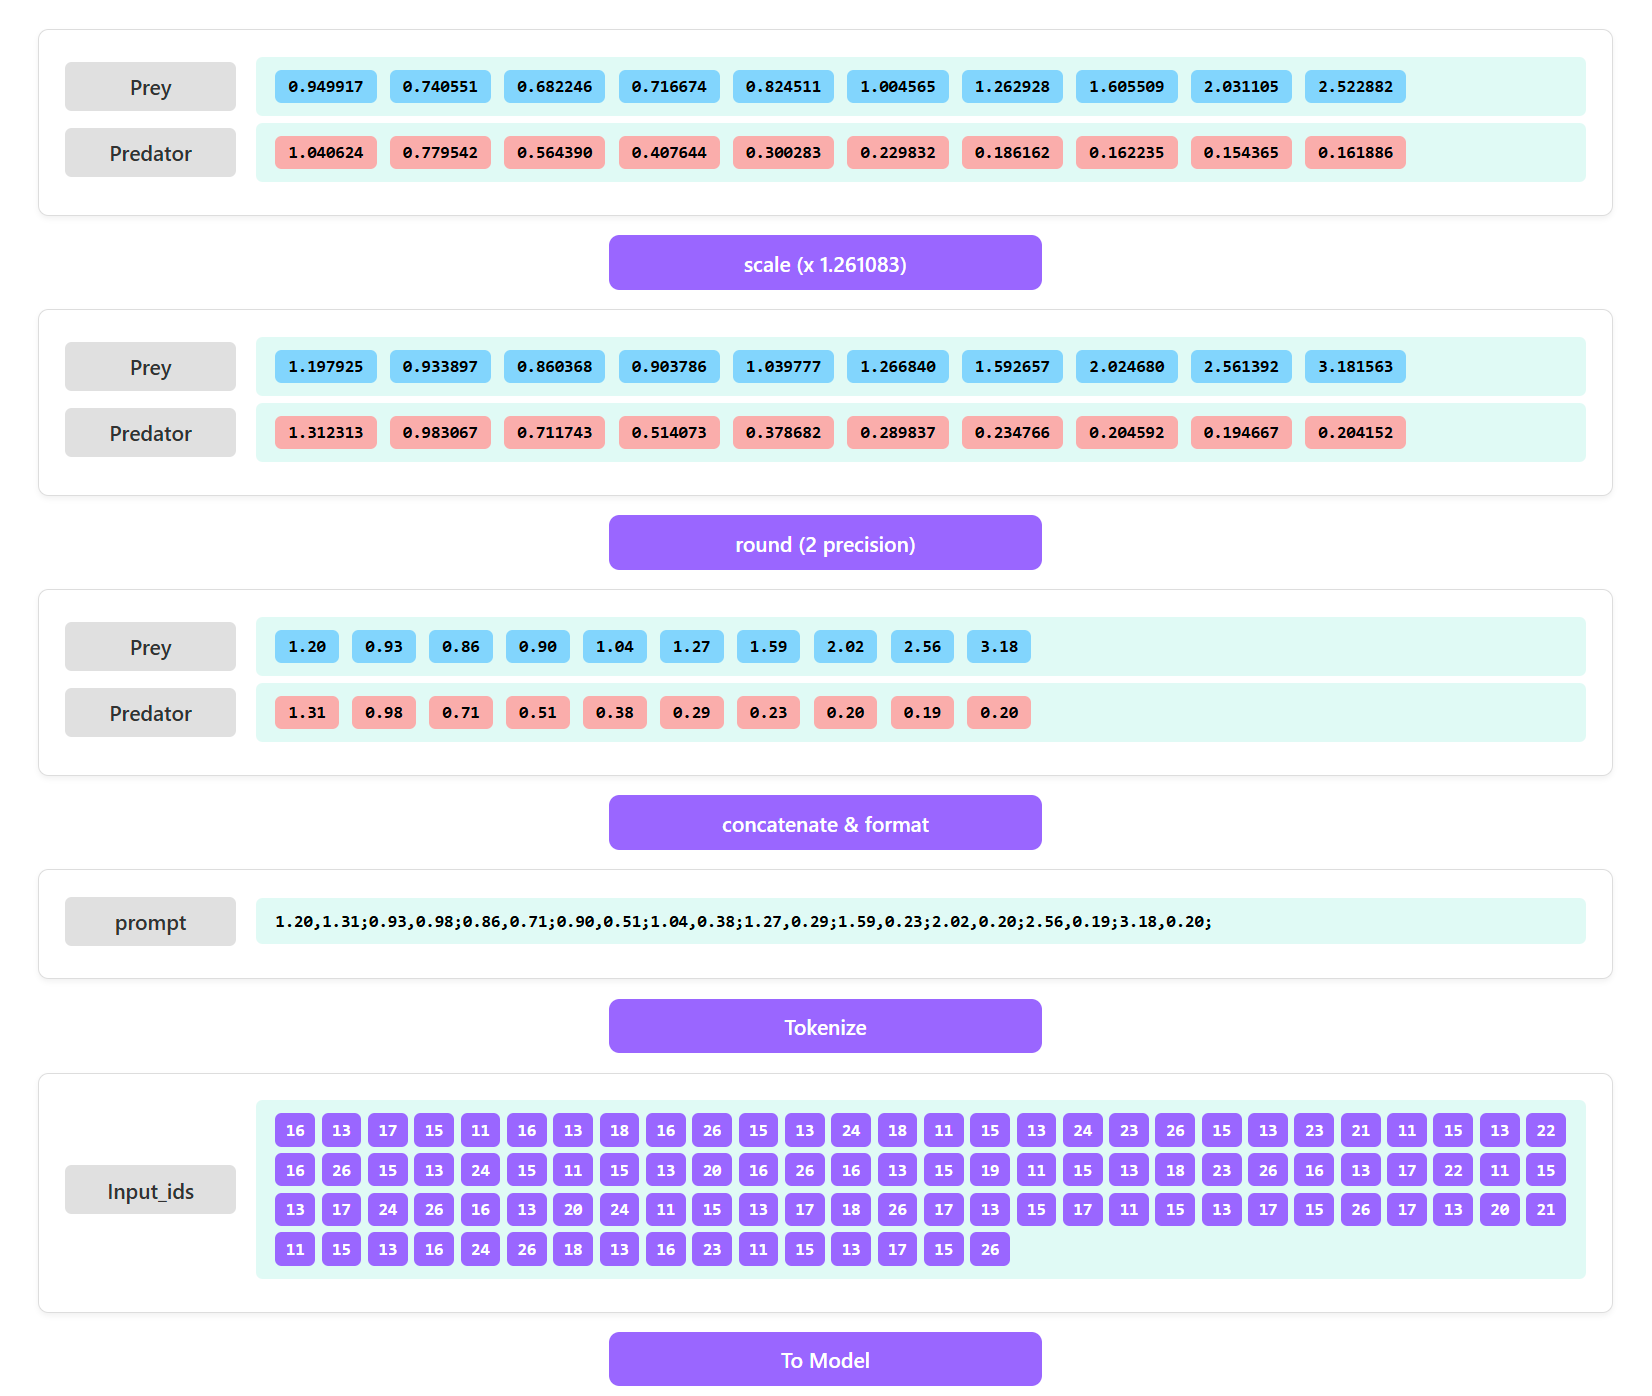
\includegraphics[width=0.9\linewidth]{M2 Course Work/Images/preprocess_vis.png} 
    \caption{Visual workflow of the time-series preprocessing steps. Raw numerical data undergoes scaling to the [0, 10] range (using a scale value of 1.26), rounding to two decimal places, and formatting into a text string. Commas separate values at the same timestamp, and semicolons separate different timestamps, creating an LLM-readable input.}
    \label{fig:preprocessing_visual_workflow}
\end{figure}

\paragraph{LLMTime Scaling Step}
The first step in preprocessing involves scaling the predator-prey time-series data to map most values within the range [0, 10]. This range is chosen to ensure a compact textual representation after rounding, facilitating more effective learning by the LLM. The scaling factor is determined using the 99.7th percentile of the dataset as an upper bound for normalization, computed as:
\begin{equation}
    \text{scaler} = \frac{10}{\text{percentile}_{99.7}(\text{data})}.
    \label{eq:scaling_factor}
\end{equation}
Using the 99.7th percentile prevents extreme outliers from disproportionately influencing the scaling factor, ensuring a robust transformation. Although the scaling steps when combined with rounding step enhance computational efficiency, they also constrain Qwen’s predictive range by making it less likely to generate values above 10. We further discuss this trade-off in the Evaluation section.


\paragraph{LLMTime Rounding Step}
After scaling, values are rounded to two decimal places. This standardization produces a consistent textual format, typically resembling \texttt{X.XX}, which improves token efficiency by reducing unnecessary token complexity. 



\paragraph{LLMTime Formatting Step}
Once scaled and rounded, the time-series data is formatted into a structured text representation. Values at each timestamp are separated by commas, while timestamps themselves are delimited by semicolons. The formatted output follows the pattern:
\begin{equation}
    p_t, h_t ; p_{t+1}, h_{t+1} ; ...
\end{equation}
where $p_t$ and $h_t$ represent prey and predator values at time $t$. This structured format maintains the temporal sequence and relationships within the data while optimizing token efficiency, reducing the computational overhead during model training and inference.

\paragraph{LLMTime Information Loss}
To assess the impact of scaling and rounding on data fidelity, we conducted a round-trip evaluation, where preprocessed data was reconstructed back into its original numerical form. Table \ref{tab:round_trip_test} presents a comparison between the original and recovered values for the first ten time steps. With a mean absolute error of only $0.002167$, the transformation introduces minimal information loss, preserving the essential characteristics of the time-series data while allowing efficient representation.









\begin{table}[!th]
\renewcommand{\arraystretch}{1.4}
\centering
\caption{Round-trip evaluation assessing information loss from the LLMTime preprocessing method (scaling, rounding, and reverse transformation). The MAE is $0.002167$. The minimal difference between original and recovered values hints that the preprocessing preserves essential signal characteristics despite significant data condensation required for Large Language Model compatibility.}
\label{tab:round_trip_test}
\footnotesize
\begin{minipage}{0.48\textwidth}
    \centering
    \caption*{\textbf{Prey Values}}
    \begin{tabular}{ccccc}
        \toprule
        \textbf{Time} \qquad & \textbf{Original} \qquad & \textbf{Processed} \qquad & \textbf{Recovered} \qquad & \textbf{Difference} \\
        \midrule
        0 & 0.949917 & 1.20 & 0.951563 & 0.001646 \\
        1 & 0.740551 & 0.93 & 0.737461 & -0.003090 \\
        2 & 0.682246 & 0.86 & 0.681954 & -0.000292 \\
        3 & 0.716674 & 0.90 & 0.713672 & -0.003002 \\
        4 & 0.824511 & 1.04 & 0.824688 & 0.000177 \\
        5 & 1.004565 & 1.27 & 1.007071 & 0.002506 \\
        6 & 1.262928 & 1.59 & 1.260821 & -0.002107 \\
        7 & 1.605509 & 2.02 & 1.601798 & -0.003711 \\
        8 & 2.031105 & 2.56 & 2.030001 & -0.001104 \\
        9 & 2.522882 & 3.18 & 2.521642 & -0.001240 \\
        \bottomrule
    \end{tabular}
\end{minipage}%
\hfill%
\begin{minipage}{0.48\textwidth}
    \centering
    \caption*{\textbf{Predator Values}}
    \begin{tabular}{ccccc}
        \toprule
        \textbf{Time} \qquad & \textbf{Original} \qquad & \textbf{Processed} \qquad & \textbf{Recovered} \qquad & \textbf{Difference} \\
        \midrule
        0 & 1.040624 & 1.31 & 1.038790 & -0.001834 \\
        1 & 0.779542 & 0.98 & 0.777110 & -0.002432 \\
        2 & 0.564390 & 0.71 & 0.563008 & -0.001382 \\
        3 & 0.407644 & 0.51 & 0.404414 & -0.003230 \\
        4 & 0.300283 & 0.38 & 0.301328 & 0.001045 \\
        5 & 0.229832 & 0.29 & 0.229961 & 0.000129 \\
        6 & 0.186162 & 0.23 & 0.182383 & -0.003779 \\
        7 & 0.162235 & 0.20 & 0.158594 & -0.003642 \\
        8 & 0.154365 & 0.19 & 0.150664 & -0.003700 \\
        9 & 0.161886 & 0.20 & 0.158594 & -0.003292 \\
        \bottomrule
    \end{tabular}
\end{minipage}
\end{table}


The LLM Preprocessor is implemented in \texttt{src\textbackslash preprocessor.py} and we also included a relevant notebook to explain this module at \href{https://gitlab.developers.cam.ac.uk/phy/data-intensive-science-mphil/assessments/m2_coursework/ym429/-/blob/main/notebooks/1_dataset_preprocess.ipynb?ref_type=heads}{\texttt{notebooks\textbackslash 1\_dataset\_preprocess.ipynb}}

\section{FLOPS Calculation}

Efficient model training is crucial, especially when operating under computational constraints. Given a FLOPS (Floating Point Operations Per Second) budget, $10^{17}$ FLOPS for the entire training process, it is necessary to accurately estimate the computational cost of training our model. This section details the FLOPS calculation methodology for the \texttt{Qwen-2.5-0.5B-Instruct} architecture configured for fine-tuning with LoRA.

\subsection{Model Architecture Overview}

To calculate the FLOPS, we first need to understand the relevant components of the \texttt{Qwen-2.5-0.5B-Instruct} architecture. This model consists of multiple identical decoder layers stacked sequentially. Based on the provided configuration and diagram (Figure \ref{fig:qwen_arch}), each Qwen decoder layer contains a Group Attention block and a Multilayer Perceptron (MLP) block. Both blocks are pre-layer-normed by RMSNorm normalization and followed by a residual connection. The overall structure and the details of key modules like Attention, MLP, and LoRA are depicted in Figure \ref{fig:qwen_arch}.

\begin{figure}[!htbp]
    \centering
    % Ensure the image path is correct
    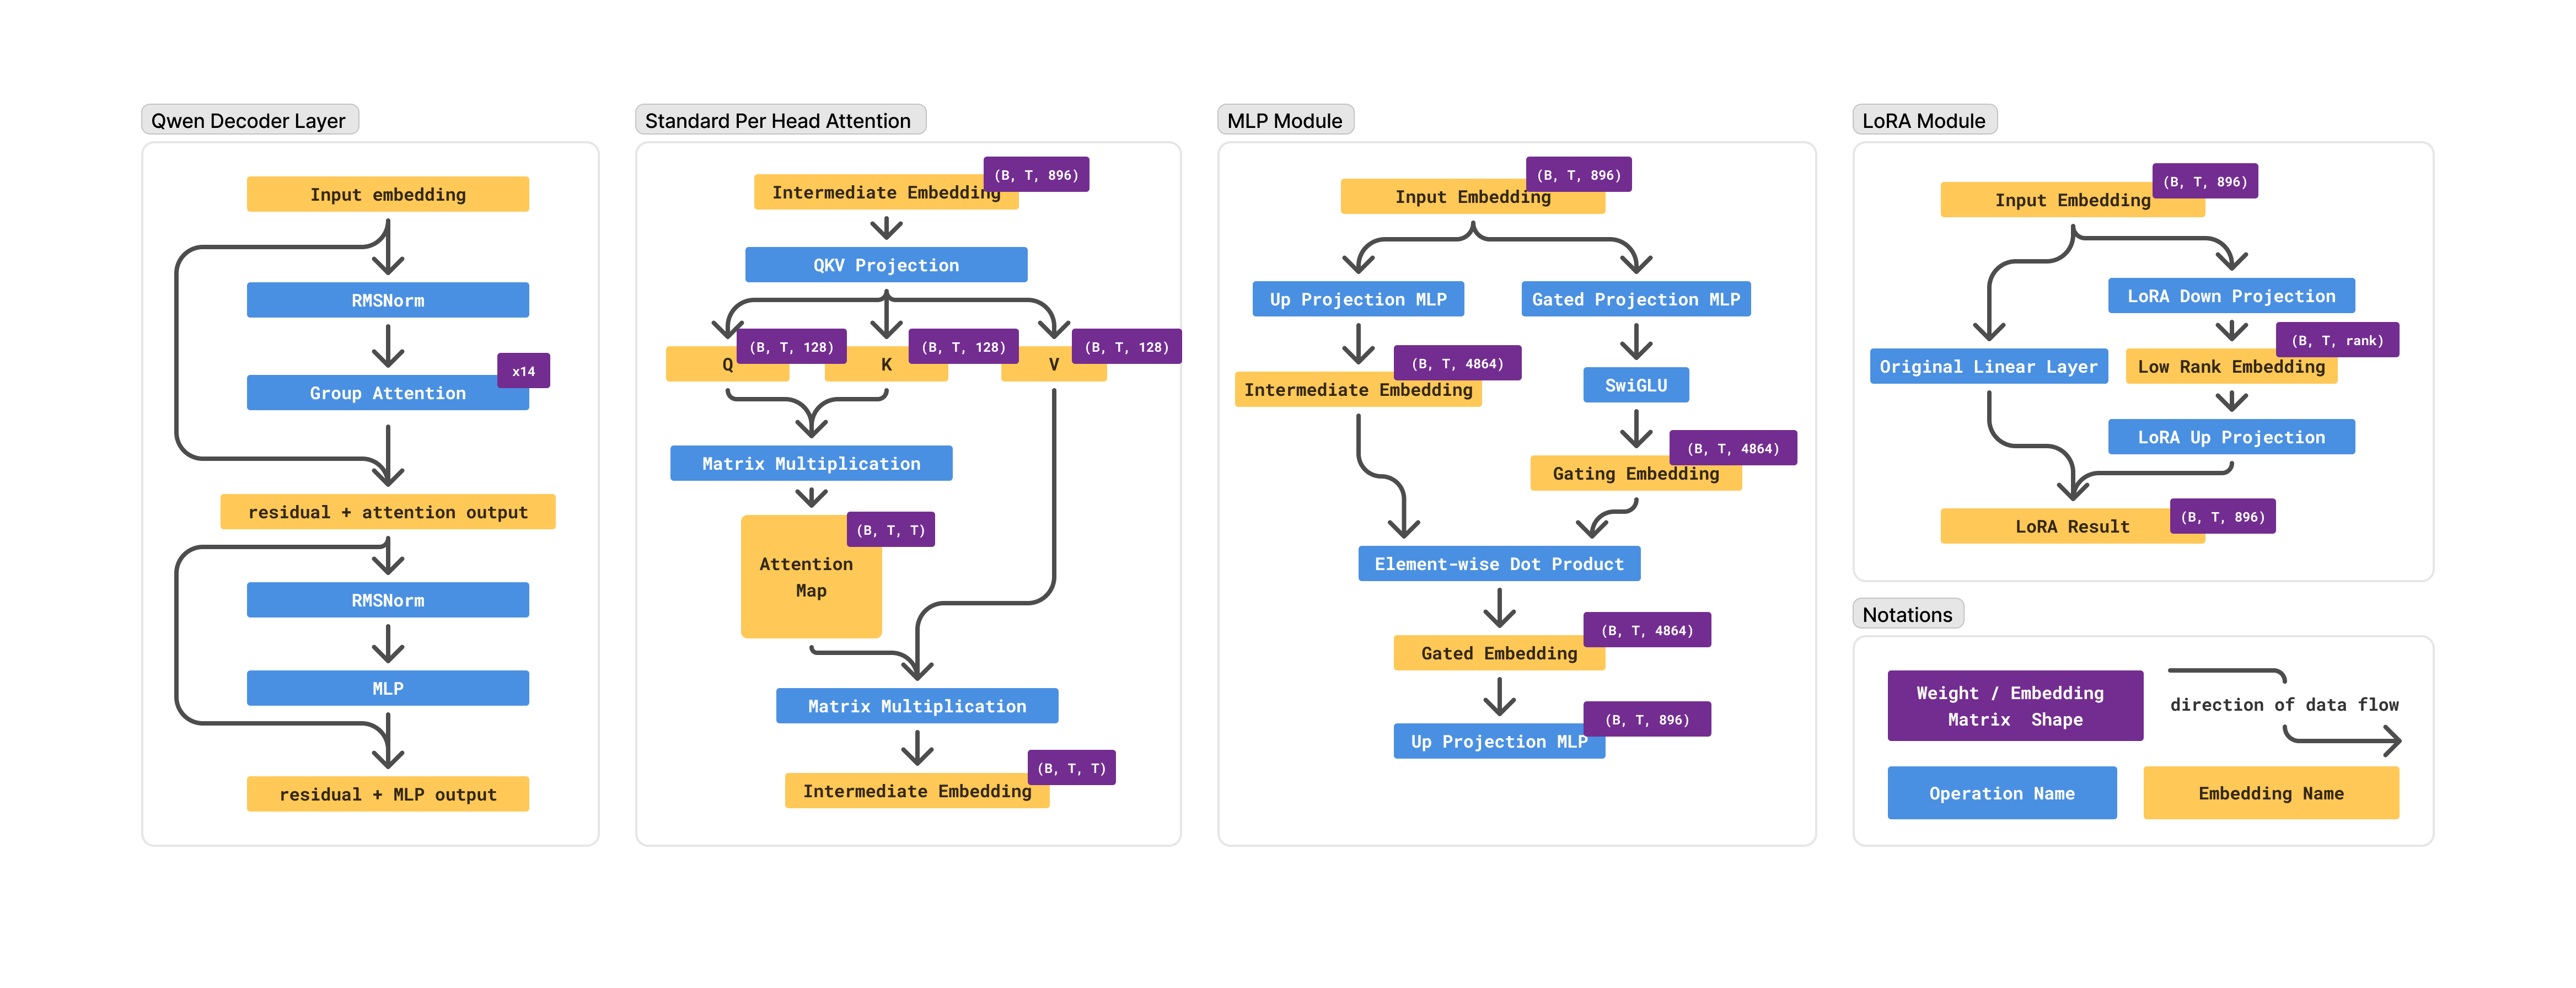
\includegraphics[width=1\linewidth]{M2 Course Work//Images/Qwen_Arch.png} 
    \caption{Architecture of a Qwen Decoder Layer and its sub-modules (Standard Per Head Attention, MLP, LoRA). Note: The Standard Attention block details standard MHA for FLOPS calculation as per coursework requirements, though the model uses Group Attention. The LoRA module illustrates its parallel application to a linear layer.}
    \label{fig:qwen_arch} 
\end{figure}


\subsection{Notation and Core Components}

To estimate the total computational cost, we adopt a component-based approach. First, we calculate the FLOPS for each distinct computational block within the Qwen decoder layer and associated operations. Then, we aggregate these individual costs based on their frequency within the overall model architecture. The primary components analyzed in this breakdown are: the RMSNorm normalization layer, the Attention mechanism (calculated using Standard Multi-Head Attention as per requirements), the MLP block (with SwiGLU activation), the additive LoRA module, the Residual Connections, and the final Language Model Head including loss computation. This analysis is based on the architecture suggested by the Hugging Face Transformers implementation of the Qwen2 model, specifically referencing the \href{https://github.com/huggingface/transformers/blob/main/src/transformers/models/qwen2/modeling_qwen2.py}{\texttt{Qwen2DecoderLayer} structure}. While this provides a concrete basis for analysis, minor variations might exist between the code implementation and theoretical diagrams or different model versions. All code and the implementation of this section can be found in \href{https://gitlab.developers.cam.ac.uk/phy/data-intensive-science-mphil/assessments/m2_coursework/ym429/-/blob/main/src/get_flops.py?ref_type=heads}{\texttt{src\textbackslash get\_flops.py}} and explained in detail in \href{https://gitlab.developers.cam.ac.uk/phy/data-intensive-science-mphil/assessments/m2_coursework/ym429/-/blob/main/notebooks/2_flops_calculation.ipynb?ref_type=heads}{\texttt{notebooks\textbackslash 1\_flops\_calculation.ipynb}}.

We use the following notation presented in Table \ref{tab:notation} for the Architecture detail, which are obtained from \href{https://huggingface.co/Qwen/Qwen2.5-0.5B-Instruct/blob/main/config.json}{Huggingface Qwen's \texttt{Config.json}}.

\begin{table}[!ht]
\renewcommand{\arraystretch}{1.3}
\centering
\setlength{\tabcolsep}{8pt}
\begin{tabular}{llc} 
    \toprule
    \textbf{Symbol} & \textbf{Description} & \textbf{Value} \\
    \midrule
    $B$           & Batch Size & 4 \\ 
    $S$           & Sequence Length & \textit{variable} \\ 
    $H$           & Hidden/Model Dimension & 896 \\
    $H_{\text{mlp}}$ & MLP Intermediate Hidden Dimension & 4864 \\
    $N_{\text{heads}}$ & Number of Attention Heads & 14 \\
    $H_{\text{head}}$ & Dimension per Attention Head ($H / N_{\text{heads}}$) & 64 \\ 
    $V_{\text{size}}$ & Vocabulary Size & 151936 \\
    $N_{\text{layers}}$ & Number of Qwen Decoder Layers & 24 \\ % Corrected symbol name to match usage
    $r$           & LoRA Rank & \textit{variable} \\ % LoRA rank is a hyperparameter
    $\alpha$      & LoRA Scaling Factor & \textit{variable} \\ % LoRA alpha is a hyperparameter
    \bottomrule
\end{tabular}
\caption{Notation for FLOPS Calculation.} 
\label{tab:notation} 
\end{table}
Additionally, We assume the FLOPS for basic arithmetic operations as in Table \ref{tab:primitive_flops}, and would reference it as $Flops_{\text{Operation Name}}$.

\begin{table}[!ht] % Changed from !th to !ht for better float placement
\renewcommand{\arraystretch}{1.4}
\centering
\setlength{\tabcolsep}{8pt} % Adjust column separation if needed
\begin{tabular}{lc}
    \toprule
    \textbf{Operation}                                 & \textbf{FLOPS} \\
    \midrule
    Addition/Subtraction/Negation (float OR integer) & 1              \\
    Multiplication/Division/Inverse (float OR integer) & 1              \\
    ReLU/Absolute Value                                & 1              \\
    Exponentiation/Logarithm                           & 10             \\
    Sine/Cosine/Square Root                            & 10             \\
    \bottomrule
\end{tabular}
\caption{FLOPS Accounting for Primitives.} % Simplified caption
\label{tab:primitive_flops}
\end{table}

\subsection{FLOPS Breakdown per Component}

\paragraph{Attention Layer (Standard MHA)}
The attention mechanism is a fundamental pillar of Transformer models. Given an input embedding $X \in \mathbb{R}^{B \times S \times H}$, it is first projected into Query ($Q$), Key ($K$), and Value ($V$) matrices using weight matrices $W_q, W_k, W_v \in \mathbb{R}^{H \times (N_{\text{heads}}H_{\text{head}})}$. 
\begin{equation}
    Q = X W_q, \quad K = X W_k, \quad V = X W_v 
\end{equation}
These resulting matrices $Q, K, V \in \mathbb{R}^{B \times S \times (N_{\text{heads}}H_{\text{head}})}$ are then typically reshaped or viewed as $N_{\text{heads}}$ individual heads, yielding $Q_i, K_i, V_i \in \mathbb{R}^{B \times S \times H_{\text{head}}}$ for $i=1, ..., N_{\text{heads}}$. Rotary Positional Embeddings (RoPE) \cite{su2023roformerenhancedtransformerrotary} are applied to $Q_i$ and $K_i$. For FLOPS calculation, we approximate the cost of RoPE primarily as element-wise operations.

The standard scaled dot-product attention is computed per head:
\begin{equation}
    \text{Attention}(Q_i, K_i, V_i) = \text{Softmax}\left(\frac{Q_i K_i^T}{\sqrt{H_{\text{head}}}}\right) V_i
\end{equation}
Although the \texttt{Qwen-2.5} model employs Grouped Query Attention (GQA), as per coursework requirements, we calculate FLOPS for standard Multi-Head Attention (MHA). The outputs from all heads are concatenated: $O = \text{Concat}(\text{Attention}_1, ..., \text{Attention}_{N_{\text{heads}}}) \in \mathbb{R}^{B \times S \times (N_{\text{heads}}H_{\text{head}})}$. This combined output $O$ is then projected back to the hidden dimension using an output weight matrix $W_o \in \mathbb{R}^{(N_{\text{heads}}H_{\text{head}}) \times H}$:
\begin{equation}
    X_{Attn} = O W_o
\end{equation}
The detailed FLOPS calculation for these operations is presented in Table \ref{tab:attention_flops}. Note that the LoRA FLOPS (Table \ref{tab:lora_flops}) are calculated separately and added where applicable (e.g., to Q and K projections).

\begin{table}[!th]
\renewcommand{\arraystretch}{1.4}
\centering
\setlength{\tabcolsep}{8pt} % Adjust column separation if needed
\begin{tabular}{ll}
    \toprule
    \textbf{Operation}                   & \textbf{Flops} \\
    \midrule
    To Q, K, V                  & $Flops_{Mul} \cdot B \cdot S \cdot H \cdot 3 \cdot 14 \cdot H_{head} +  Flops_{Add} \cdot B \cdot S \cdot (H -1) \cdot 3 \cdot 14 \cdot H_{head}$ \\
    Add ROPE                    & $Flops_{Add} \cdot B \cdot S \cdot 3 \cdot 14 \cdot H_{head}$ \\ % Note: Code comment suggests 2* instead of 3*
    $QK^T$                      & $Flops_{Mul} \cdot B \cdot 14 \cdot S \cdot H_{head} \cdot S +  Flops_{Add} \cdot B \cdot 14 \cdot S \cdot (H_{head}-1) \cdot S$ \\
    divide by $\sqrt{H_{head}}$ & $Flops_{SQRT} + Flops_{DIV} \cdot B \cdot S \cdot S \cdot H_{head}$ \\ % Note: Discrepancy with code comment structure
    Adding Attention Mask       & $Flops_{Add} \cdot B \cdot S \cdot S \cdot H_{head}$ \\ % Note: Discrepancy with code comment (missing 14, H_head)
    Softmax                     & $(Flops_{EXP} + Flops_{DIV}) \cdot B \cdot S \cdot S \cdot H_{head} + (Flops_{ADD}) \cdot B \cdot S \cdot (S-1) \cdot H_{head}$ \\ % Note: Discrepancy with code comment structure
    multiply by V               & $Flops_{MUL} \cdot B \cdot 14 \cdot S \cdot S \cdot H_{head} + Flops_{ADD} \cdot B \cdot 14 \cdot S \cdot (S - 1) \cdot H_{head}$ \\
    multiply by $w_o$           & $Flops_{MUL} \cdot B \cdot S \cdot H \cdot (14 \cdot H_{head}) + Flops_{ADD} \cdot  B \cdot S \cdot H \cdot (14 \cdot H_{head} - 1)$ \\ % Rewrote slightly for clarity based on code logic
    \bottomrule
\end{tabular}
\caption{FLOPs Breakdown for Attention Mechanism Layer}
\label{tab:attention_flops}
\end{table}

\paragraph{RMSNorm}
RMSNorm \cite{zhang2019rootmeansquarelayer} is a computationally efficient normalization technique. Given an input $x \in \mathbb{R}^{B \times S \times H}$, it normalizes the input across the hidden dimension $H$. As it is only across the hidden dimension, we can simplify the problem and consider that for a vector $x \in \mathbb{R}^H$, the normalization is:
\begin{equation}
    \text{RMS}(x) = \sqrt{\frac{1}{H} \sum_{i=1}^{H} x_i^2 + \epsilon}
\end{equation}
\begin{equation}
    y_i = \frac{x_i}{\text{RMS}(x)} \gamma_i
\end{equation}
where $\gamma \in \mathbb{R}^H$ is a learnable scaling parameter and $\epsilon$ is a small constant for numerical stability. This calculation is applied independently to each token's hidden vector across the batch. The FLOPS are detailed in Table \ref{tab:rmsnorm_flops}.

\begin{table}[!th]
\renewcommand{\arraystretch}{1.4}
\centering
\setlength{\tabcolsep}{8pt} % Adjust column separation if needed
\begin{tabular}{ll}
    \toprule
    \textbf{Operation}                     & \textbf{Flops} \\
    \midrule
    Square elements in embedding               & $Flops_{Mul} \cdot B \cdot S \cdot H$ \\
    Mean over Hidden dimension of the embedding & $Flops_{Add} \cdot B \cdot S \cdot (H - 1) + Flops_{Div} \cdot B \cdot S$ \\
    Add epsilon                   & $Flops_{Add} \cdot B \cdot S$ \\
    Calculate sqrt (for rsqrt)    & $Flops_{Sqrt} \cdot B \cdot S$ \\
    Calculate reciprocal (for rsqrt)& $Flops_{Div} \cdot B \cdot S$ \\
    Multiply embedding by rsqrt & $Flops_{Mul} \cdot B \cdot S \cdot H$ \\
    Multiply by weight  $\gamma$          & $Flops_{Mul} \cdot B \cdot S \cdot H$ \\
    \bottomrule
\end{tabular}
\caption{FLOPs Breakdown for RMSNorm Layer}
\label{tab:rmsnorm_flops}
\end{table}


\paragraph{MLP Module (SwiGLU)}
The MLP module in Qwen uses a SwiGLU (SiLU-Gated Linear Unit) structure \cite{shazeer2020gluvariantsimprovetransformer}. Given an input $x \in \mathbb{R}^{B \times S \times H}$, it involves two linear projections to the intermediate dimension $H_{\text{mlp}}$ using weight matrices $W_{up}, W_{gate} \in \mathbb{R}^{H \times H_{\text{mlp}}}$. The SiLU activation ($\text{SiLU}(z) = z \cdot \text{sigmoid}(z)$) is applied to the gate projection, followed by element-wise multiplication to the up projected embedding. Finally, a down-projection using $W_{down} \in \mathbb{R}^{H_{\text{mlp}} \times H}$ maps the result back to the hidden dimension $H$.
\begin{equation}
    X_{MLP} = \left[ (X W_{up}) \odot \text{SiLU}(X W_{gate}) \right] W_{down}
\end{equation}
The FLOPS breakdown is shown in Table \ref{tab:ffn_glu_flops}.

\begin{table}[!th]
\renewcommand{\arraystretch}{1.4}
\centering
\setlength{\tabcolsep}{8pt} % Adjust column separation if needed
\begin{tabular}{ll}
    \toprule
    \textbf{Operation}                   & \textbf{Flops} \\
    \midrule
    Gate Projection             & $Flops_{Mul} \cdot B \cdot S \cdot H \cdot H_{mlp} + Flops_{Add} \cdot B \cdot S \cdot (H - 1) \cdot H_{mlp}$ \\
    SiLU Activation   & $(Flops_{Neg} + Flops_{Exp} + Flops_{Add} + Flops_{Div} + Flops_{Mul}) \cdot B \cdot S \cdot H_{mlp}$ \\
    Up Projection               & $Flops_{Mul} \cdot B \cdot S \cdot H \cdot H_{mlp} + Flops_{Add} \cdot B \cdot S \cdot (H - 1) \cdot H_{mlp}$ \\
    Element-wise Mult (Gate*Up) & $Flops_{Mul} \cdot B \cdot S \cdot H_{mlp}$ \\
    Down Projection             & $Flops_{Mul} \cdot B \cdot S \cdot H_{mlp} \cdot H + Flops_{Add} \cdot B \cdot S \cdot (H_{mlp} - 1) \cdot H$ \\
    \bottomrule
\end{tabular}
\caption{FLOPs Breakdown for Multi-layer Perception Layer with SwiGLU}
\label{tab:ffn_glu_flops}
\end{table}

\paragraph{Low Rank Adaptation (LoRA)}
LoRA \cite{hu2021loralowrankadaptationlarge} is a parameter-efficient fine-tuning. LoRA works by freezing the entire Qwen model, and then injecting two low rank tunable weight matrices to each linear layer of q and k projection layer in the Multi-headed Attention Layers. These low rank weight matrices affectively mimics the fine-tuning weight update, thereby allows affective and efficient fine-tuning with only a fraction of parameter size.

For an input $x$, the output of a LoRA-adapted linear layer is 
\begin{equation}
    y = xW + x A B (\alpha / r),
\end{equation}
where $A \in \mathbb{R}^{d_{in} \times r}$ and $B \in \mathbb{R}^{r \times d_{out}}$ are the trainable low-rank matrices, $r$ is the rank, and $\alpha$ is a scaling factor.  Table \ref{tab:lora_flops} details the FLOPS associated only with the LoRA path ($x A B (\alpha / r)$), which represents the additional computational cost incurred by using LoRA. For Q/K projections, $d_{in}=H$ and $d_{out}={H_{head}N_{heads}}$.

\begin{table}[!th]
\renewcommand{\arraystretch}{1.4}
\centering
\setlength{\tabcolsep}{8pt} % Adjust column separation if needed
\begin{tabular}{ll}
    \toprule
    \textbf{Operation}       & \textbf{Flops} \\
    \midrule
    Down Projection  (A)  & $Flops_{Mul} \cdot B \cdot S \cdot H \cdot R + Flops_{Add} \cdot B \cdot S \cdot (H - 1) \cdot R$ \\
    Up Projection   (B)   & $Flops_{Mul} \cdot B \cdot S \cdot R \cdot H_{head} \cdot 14 + Flops_{Add} \cdot B \cdot S \cdot (R - 1) \cdot H_{head} \cdot 14$ \\
    Scaling Output     & $Flops_{Mul} \cdot B \cdot S \cdot H_{head} \cdot 14$ \\
    Addition to Orig   & $Flops_{Add} \cdot B \cdot S \cdot H_{head} \cdot 14$ \\
    \bottomrule
\end{tabular}
\caption{FLOPs Breakdown for LoRA Layer}
\label{tab:lora_flops}
\end{table}


\paragraph{Residual Connection}
Residual connections add the input of a block (e.g., Attention or MLP) to its output. This involves a simple element-wise addition, crucial for training deep networks.
\begin{equation}
    X_{out} = X_{in} + \text{Block}(X_{in})
\end{equation}
The associated FLOPS are shown in Table \ref{tab:residual_flops}.

\begin{table}[!th]
\renewcommand{\arraystretch}{1.4}
\centering
\setlength{\tabcolsep}{8pt} % Adjust column separation if needed
\begin{tabular}{ll}
    \toprule
    \textbf{Operation}           & \textbf{Flops} \\
    \midrule
    Residual Connection & $Flops_{Add} \cdot B \cdot S \cdot H$ \\
    \bottomrule
\end{tabular}
\caption{FLOPs Breakdown for Residual Connection}
\label{tab:residual_flops}
\end{table}


\paragraph{LLM Head and Loss Calculation}
After the final decoder layer, the output embedding $X_{final} \in \mathbb{R}^{B \times S \times H}$ is projected to the vocabulary dimension using an LM head weight matrix $W_{LLM} \in \mathbb{R}^{H \times V_{\text{size}}}$ to produce logits.
\begin{equation}
    \text{Logits} = X_{final} W_{LLM} + b_{LLM}
\end{equation}
A Softmax function is applied to the logits to obtain token probabilities, and typically a Cross-Entropy loss is computed against the target tokens. Table \ref{tab:lm_head_flops} outlines the FLOPS for the LM head projection and a simplified view of the subsequent Softmax and loss calculation steps.

\begin{table}[!th]
\renewcommand{\arraystretch}{1.4}
\centering
\setlength{\tabcolsep}{8pt} % Adjust column separation if needed
\begin{tabular}{ll}
    \toprule
    \textbf{Operation}        & \textbf{Flops} \\
    \midrule
    LM Head (MatMul) & $Flops_{Mul} \cdot B \cdot S \cdot H \cdot V_{size} + Flops_{Add} \cdot B \cdot S \cdot (H - 1) \cdot V_{size}$ \\
    LM Head (Bias)   & $Flops_{Add} \cdot B \cdot S \cdot V_{size}$ \\
    Softmax          & $(Flops_{Exp} + Flops_{Add} + Flops_{Div}) \cdot B \cdot S \cdot V_{size}$ \\
    Log \& Multiply    & $(Flops_{Log} + Flops_{Mul}) \cdot B \cdot S$ \\ % Added \& for ampersand
    \bottomrule
\end{tabular}
\caption{FLOPs Breakdown for LM Head and Final Operations}
\label{tab:lm_head_flops}
\end{table}


\subsection{Total FLOPS Estimation}

With the FLOPS for each component defined, we can assemble the total FLOPS for one forward pass through a single Qwen decoder layer. Assuming LoRA is applied to both Q and K projections within the attention block:
\begin{align}
Flops_{\text{Qwen Decoder Layer}} &=  Flops_{\text{RMSNorm}} \nonumber \\
                                 &+ (Flops_{\text{Attention}} + 2 \times Flops_{\text{LoRA}} ) \nonumber \\ 
                                 &+ Flops_{\text{Residual}} \nonumber \\
                                 &+Flops_{\text{RMSNorm}} \nonumber\\
                                 &+ Flops_{\text{FFN}} \nonumber \\
                                 &+ Flops_{\text{Residual}} \label{eq:qwen_layer_flops}
\end{align}


The total FLOPS for a single forward pass (inference) through the entire $N_{\text{layers}}=24$ model is:
\begin{equation}
Flops_{\text{Qwen Inference}} = N_{\text{layers}} \times Flops_{\text{Qwen Decoder Layer}} + Flops_{\text{LM Head + Loss}}
\label{eq:qwen_inference_flops}
\end{equation}
where $Flops_{\text{LM Head + Loss}}$ represents the sum of operations listed in Table \ref{tab:lm_head_flops}.

For training, we need to account for both the forward pass and the backward pass, we here approximate the backward pass as twice the computation of the forward pass. Therefore, the total FLOPS for one training step is:
\begin{equation}
Flops_{\text{Qwen Training Step}} \approx 3 \times Flops_{\text{Qwen Inference}}
\label{eq:qwen_training_flops}
\end{equation}
This estimate provides the basis for calculating the total computational cost over the course of training by multiplying with the number of training steps.


\subsection{Experiment Planning within FLOPS Budget}

Having established a method for calculating FLOPS per training step (Equation \ref{eq:qwen_training_flops}), we can now plan our experiments realistically within the given total computational budget of $1 \times 10^{17}$ FLOPS. This budget must cover all experimental runs, including hyperparameter searches and the final model training.

First, we calculated the FLOPS cost per training step for various anticipated configurations, specifically varying the sequence context length ($S$) and the LoRA rank ($r$), while keeping the batch size fixed at $B=4$. Table \ref{tab:flops_vs_steps} presents these per-step FLOPS costs.

\begin{table}[!th]
\renewcommand{\arraystretch}{1.4}
\centering
\setlength{\tabcolsep}{8pt} % Adjust column separation if needed
\begin{tabular}{ccrr}
    \toprule
    \textbf{Context Length} & \textbf{Rank} & \textbf{Total FLOPs} & \textbf{Optimizer Steps} \\
    \midrule
    128 & 2 &  1,896,002,957,196 & 52,743 \\
    128 & 4 &  1,896,179,031,948 & 52,738 \\
    128 & 8 &  1,896,531,181,452 & 52,728 \\
    \midrule % Optional: Add rule to separate context lengths visually
    512 & 2 &  8,000,191,522,188 & 12,500 \\
    512 & 4 &  8,000,895,821,196 & 12,499 \\
    512 & 8 &  8,002,304,419,212 & 12,496 \\
    \midrule % Optional: Add rule to separate context lengths visually
    768 & 2 & 12,416,467,077,516 & 8,054 \\
    768 & 4 & 12,417,523,526,028 & 8,053 \\
    768 & 8 & 12,419,636,423,052 & 8,052 \\
    \bottomrule
\end{tabular}
\caption{Calculated FLOPS per training step and the corresponding maximum affordable optimizer steps within a $1 \times 10^{17}$ total FLOPS budget for different configurations (Batch Size $B=4$).}
\label{tab:flops_vs_steps}
\end{table}

Given that the total budget must accommodate multiple experiments, including approximately 12 grid search runs (exploring learning rates, ranks, and potentially context lengths) and one larger final training run to develop the best model's potential, we designed a step allocation strategy. Table \ref{tab:training_steps} outlines the planned number of optimizer steps for each phase of our experimental procedure.

\begin{table}[!htbp] % Changed from !th to !htbp
\renewcommand{\arraystretch}{1.4}
\centering
\setlength{\tabcolsep}{8pt} 
\begin{tabular}{lr}
    \toprule
    \textbf{Training Phase}           & \textbf{Planned Optimizer Steps} \\ % Clarified column header
    \midrule
    Initial Training / Smoke Test      & 1,000 \\
    Grid Search Runs (per run)\textsuperscript{a}  & 500 \\
    % Grid Search (Context Length) & 500 \\ % Merged into grid search runs or clarify if separate
    Final Model Training            & $\approx$ 3,000\textsuperscript{b} \\ % Used \approx for clarity
    \bottomrule
\end{tabular}
\caption{Planned optimizer step allocation for different training phases. \newline 
\textsuperscript{a}Applies to each of the 12 grid search experiments exploring learning rate, LoRA rank, and context length. \newline 
\textsuperscript{b}The final training is flexible, utilizing the remaining FLOPS budget after grid search, estimated to be between 2,000 - 4,000 steps depending on the configurations used during search.}
\label{tab:training_steps}
\end{table}

This allocation strategy allows small scale experiment to explore the hyper-parameter, while reserving a significant portion of the FLOPS budget for training the final selected model.



\section{Experimental Setup and Data Preparation}

Our experiment have four main phases: 
\begin{enumerate}
    \item An initial training run using default hyperparameters provided in the course skeleton code to establish a baseline.
    \item A grid search phase exploring different LoRA ranks and learning rates.
    \item Another search over different input context lengths.
    \item A final, extended training phase using the best configuration identified from the previous phases to maximize model performance within the FLOPS budget.
\end{enumerate}

\subsection{Data Processing and Formatting}

The dataset was first partitioned into training (80\%), validation (10\%), and testing (10\%) sets to ensure robust evaluation on unseen data. Each system's time series data was then formatted into tokens using LLMTime Preprocessing procedure stated in Section \ref{sec:preprocessing}. This process resulted in sequences of approximately 1000 tokens per system. Given the sequence length limitations of transformer models, these long sequences were subsequently divided into smaller chunks of a specified context length ($S \in \{128, 512, 768\}$). To maximize data utilization, we used a sliding window approach with a stride of 256 tokens, generating overlapping sequences for training and evaluation.

\subsection{Handling Padding for Qwen}
\label{sec:padding}

A key challenge during setup was input sequence padding. The provided \textit{LoRA skeleton} used right-padding by default, but the \textit{Qwen} model was trained with left-padding. This mismatch disrupted causal attention and positional encoding, causing the model to generate incoherent outputs instead of numerical predictions (Figure \ref{fig:padding_effect}). The issue was identified after main experiments, so a workaround was used: only full-length sequences were retained, while shorter sequences were discarded. The impact of this exclusion on generalization is discussed in Section \ref{sec:disscusion}.

% A critical challenge encountered during setup involved input sequence padding. Padding is often used when batching sequences of varying lengths to ensure uniform tensor dimensions. The provided \texttt{LoRA skeleton} code implemented right-padding by default. However, applying this to the \texttt{Qwen} model resulted in problematic outputs, where the model generated incoherent natural language instead of the expected numerical predictions, as illustrated in the top panel of Figure \ref{fig:padding_effect}.

% Further investigation revealed that the pre-trained \texttt{Qwen} model family was originally trained using \textbf{left-padding}. Transformer models, particularly decoder-only architectures like Qwen, can be sensitive to padding direction as it affects the causal attention mask and positional encoding interpretation. Fine-tuning with right-padding creates a mismatch, which could leads to potential model failure. The middle and bottom panels of Figure \ref{fig:padding_effect} show that both using no padding (with full-context-length sequences) or the correct left-padding allows the model to generate outputs in the expected numerical format.

% Unfortunately, the requirement for left-padding was discovered only after the main experiments were completed. And I was using a workaround: only sequences with full chunks not requiring any padding were retained for training and evaluation. Shorter sequences resulting from the chunking process, primarily at the end of each system's data, were discarded. While this ensures the model processes sequences without padding interference, the potential impact of excluding these shorter, potentially informative sequences on the model's generalization performance will be further disscussed in section \ref{sec:disscusion}.


\begin{figure}[!htbp] % Use positioning options like htbp
    \centering
    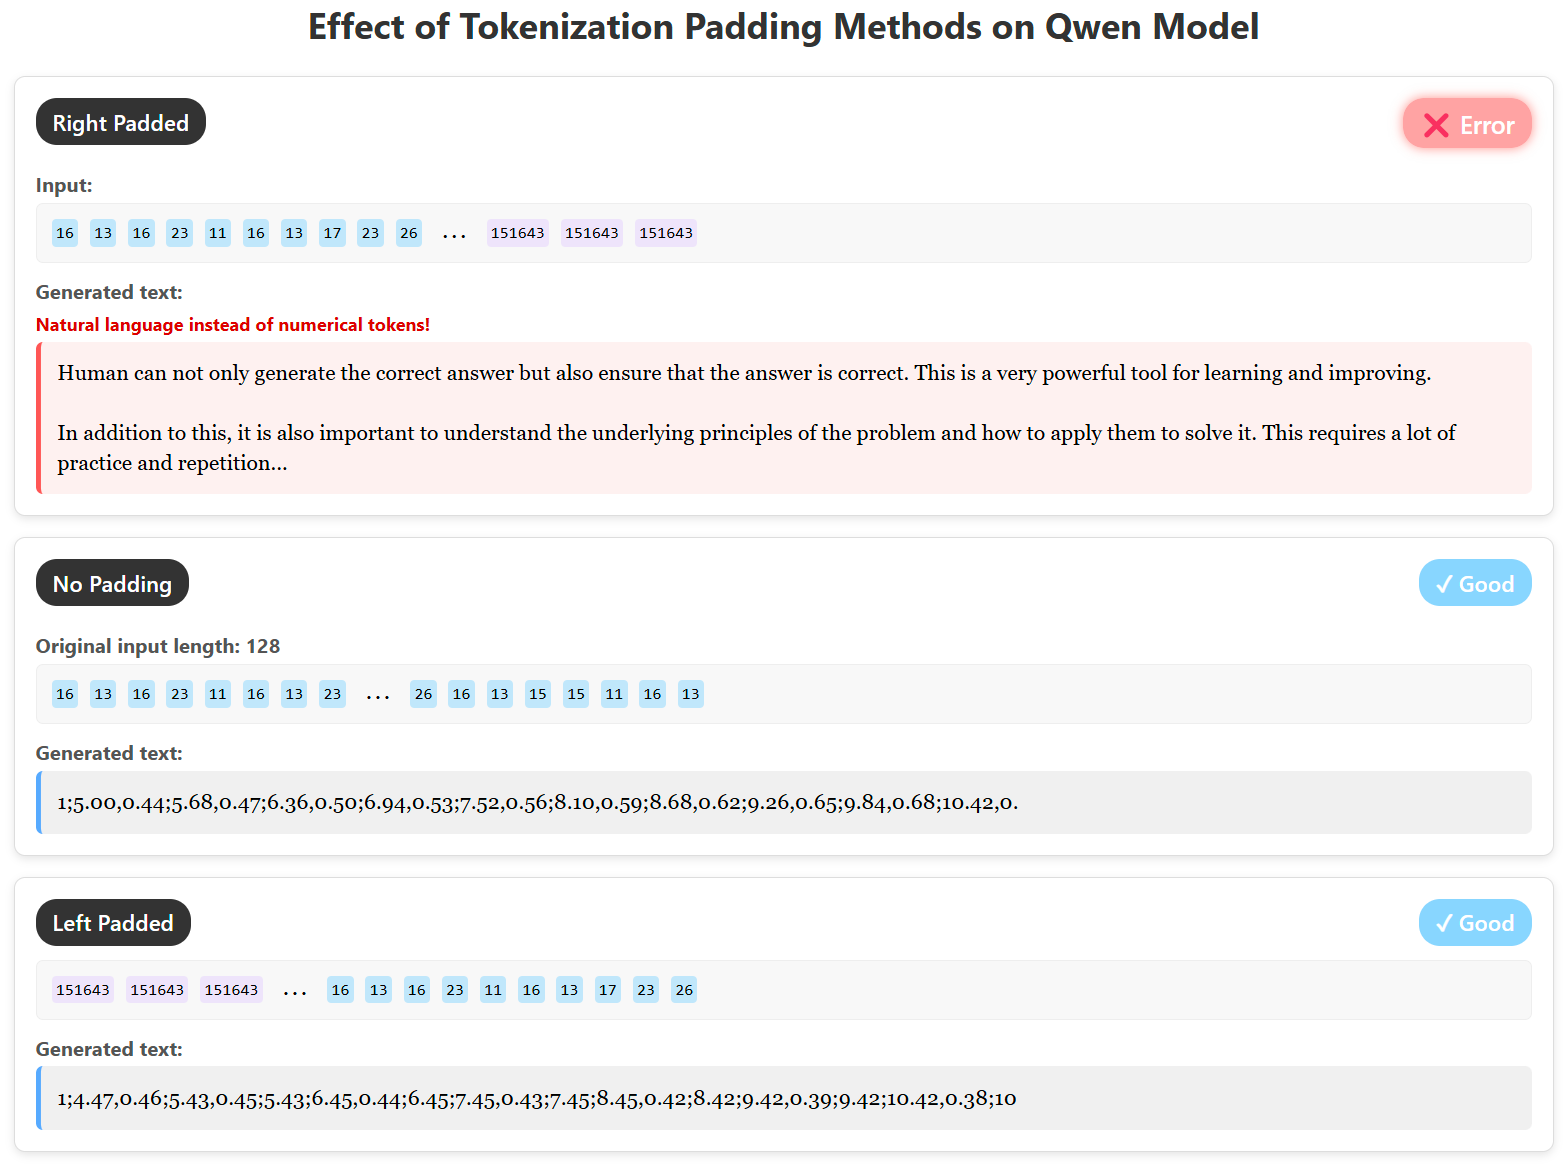
\includegraphics[width=0.9\linewidth]{M2 Course Work//Images/padding_effect.png} % Adjusted width slightly
    \caption{Effect of different padding strategies on the \texttt{Qwen} model's output for the predator-prey numerical sequence generation task. Top panel: Right-padding (default in skeleton code) causes the model to fail, generating erroneous natural language. Middle panel: Using only full sequences (no padding needed) results in the correct numerical output format. Bottom panel: Left-padding (the strategy Qwen was pre-trained with) also produces the correct numerical format.}
    \label{fig:padding_effect}
\end{figure}

\subsection{Training and Evaluation}

For all experiment, we evaluate the model every 50 training steps on the validation set, and keep the best performing models for evaluation based on the based on validation loss. The model are then evaluated based on the divination of decoded sequence from the target sequence measuerd by MSE and MAE. 
\begin{figure}
    \centering
    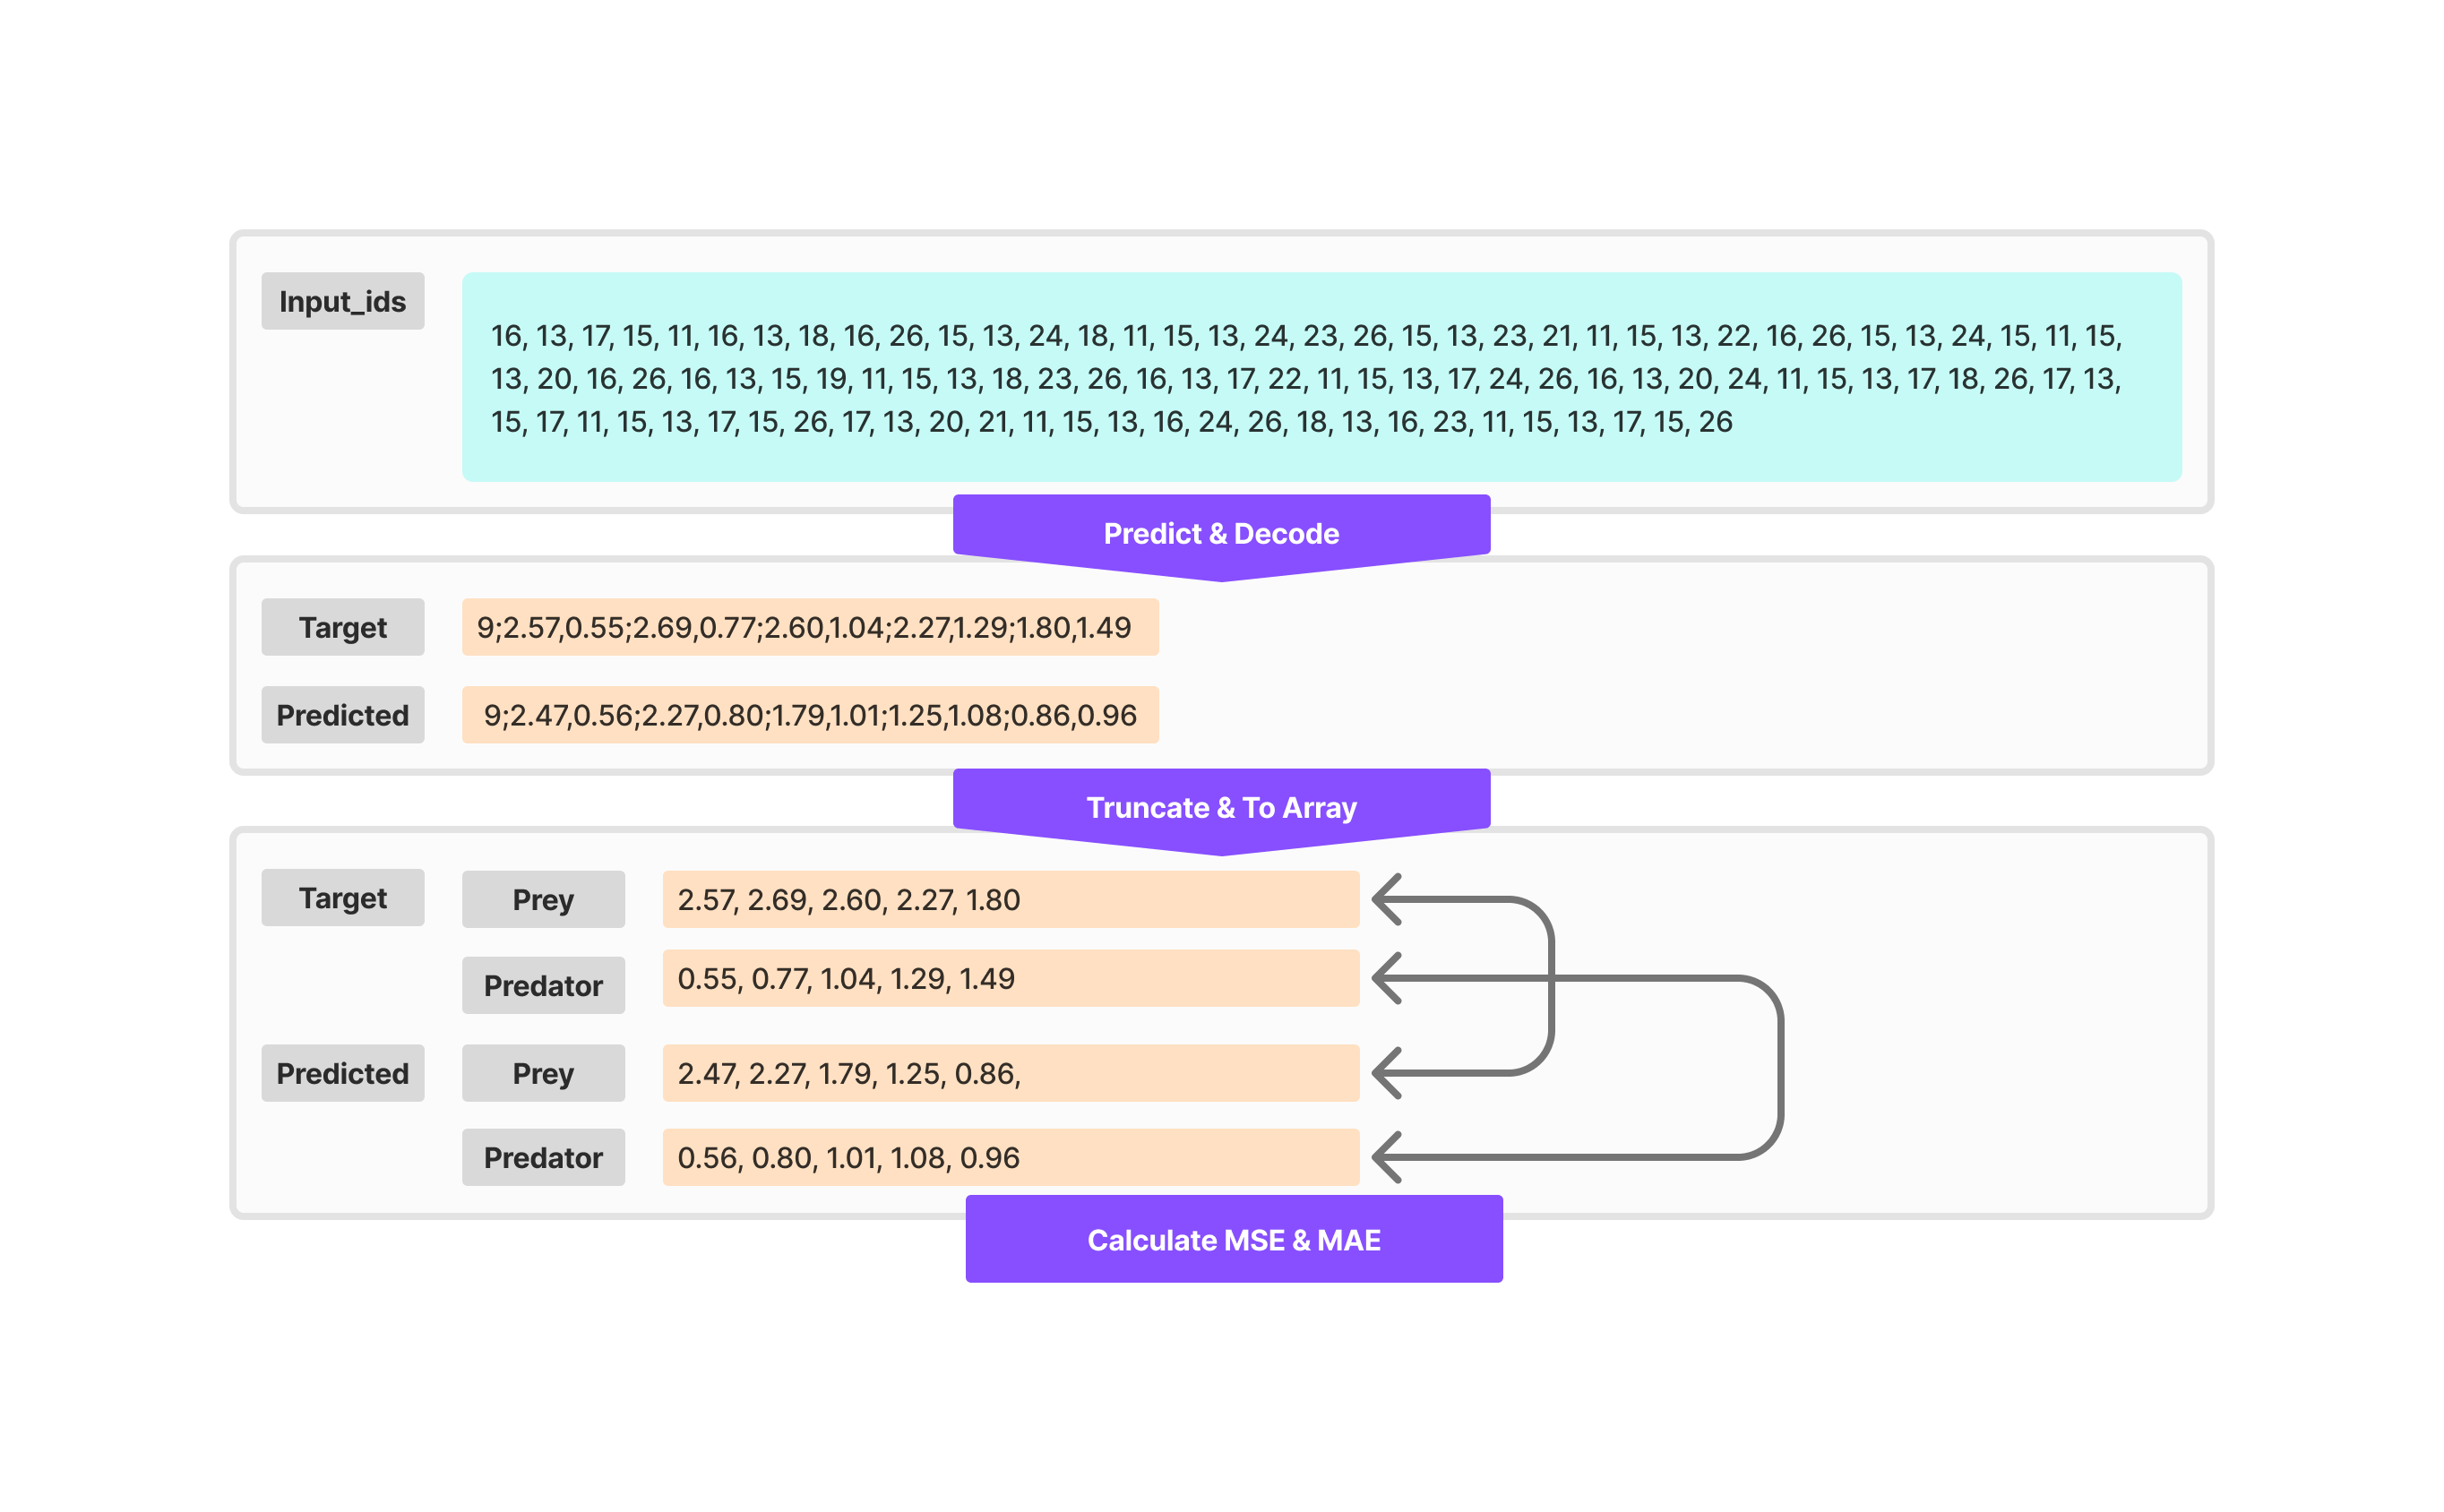
\includegraphics[width=1\linewidth]{M2 Course Work//Images/Metric_calculation.png}
    \caption{Enter Caption}
    \label{fig:metric-calculation}
\end{figure}

Given that predicting up to the first time stamp may not be significant enough as seen in Figure \ref{fig:metric-diff-between-timestamp}. As the model continously predicting based on its prior predicition, the result would degrad over time, thus showcasing a more pronounced difference in performance. Therefore, based on  Figure \ref{fig:metric-diff-between-timestamp}, we would say that predicitng up to 5 th time stamp would have enough difference between, thus we allow all experiment during the final evaluation, we let the model predict until the 5th timestamp, and then do the MSE and MAE calcualtion. We will present the average of all test data's perfroamance over avergae of all these 5 time stamp when report MSE and MAE.

\begin{figure}
    \centering
    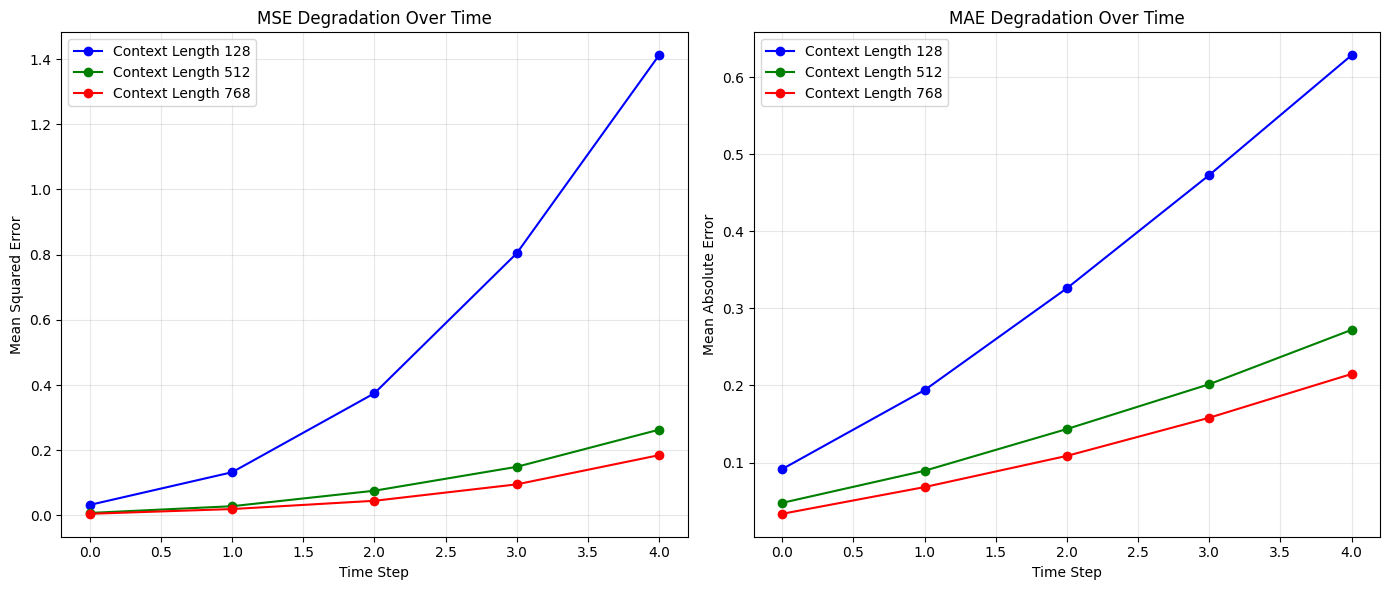
\includegraphics[width=1\linewidth]{M2 Course Work//Images/metric_diff_between_timestamp.png}
    \caption{Untrained performance on different context length. }
    \label{fig:metric-diff-between-timestamp}
\end{figure}


\section{Results}

This section details the performance of the \texttt{Qwen} model across different stages of training, evaluating its ability to learn the predator-prey dynamics.

\subsection{Untrained Baseline Performance}

Before any fine-tuning, we evaluated the zero-shot performance of the pre-trained \texttt{Qwen} model on the test set. The objective was to establish a baseline and understand the model's initial capabilities on this specialized numerical task. Mean Squared Error (MSE) and Mean Absolute Error (MAE) were calculated for different input context lengths, as shown in the Untrained section of Table \ref{tab:training_stage_comparison}.

\begin{table}[!th]
\renewcommand{\arraystretch}{1.4}
\centering
\setlength{\tabcolsep}{8pt}
\sisetup{round-mode=places, round-precision=6} % Optional: To align numbers by decimal point using S column type
% If using siunitx for alignment, the column spec would be c S[table-format=1.6] S[table-format=1.6] S[table-format=1.6] S[table-format=1.6] S[table-format=1.6] S[table-format=1.6]
% However, sticking to the simpler rr format for now as requested by the original style.
\begin{tabular}{c rr rr rr}
    \toprule
    & \multicolumn{2}{c}{\textbf{Untrained}}
    & \multicolumn{2}{c}{\textbf{Initial Training}} % More descriptive
    & \multicolumn{2}{c}{\textbf{Final Training}} \\ % More descriptive
    \cmidrule(lr){2-3} \cmidrule(lr){4-5} \cmidrule(lr){6-7}
    \textbf{Context Length ($S$)} & \textbf{MSE} & \textbf{MAE} & \textbf{MSE} & \textbf{MAE} & \textbf{MSE} & \textbf{MAE} \\
    \midrule
    128 & 0.551002 & 0.342673 & 0.135554 & 0.174634 & 0.026321 & 0.072551 \\
    512 & 0.104814 & 0.150884 & 0.036210 & 0.083372 & 0.002771 & 0.023984 \\
    768 & 0.069979 & 0.116683 & 0.029675 & 0.065142 & 0.002024 & 0.019064 \\
    \bottomrule
\end{tabular}
\caption{Comparison of test set performance (MSE and MAE) across different training stages and context lengths. Initial training involved 1000 steps ($S=512, \eta=10^{-4}, r=4$). Final training used the optimal configuration ($\eta=10^{-4}, r=8, S=768$).}
\label{tab:training_stage_comparison}
\end{table}

The metrics indicate poor initial performance, as expected for a model pre-trained on natural language and applied to a numerical time-series task. However, there is a clear trend: performance improves (lower MSE and MAE) as the context length increases, suggesting the model leverages longer historical information, even without specific training. Visual inspection of predictions (Figure \ref{fig:untrained_predictions}) further confirmed the model's lack of understanding of the dynamics; when asked to predict the next 20 time steps, the outputs were effectively constant or near-constant values, failing to capture any cyclical or dynamic structure present in the true data.

\begin{figure}[!htbp] % Use htbp for better placement
    \centering
    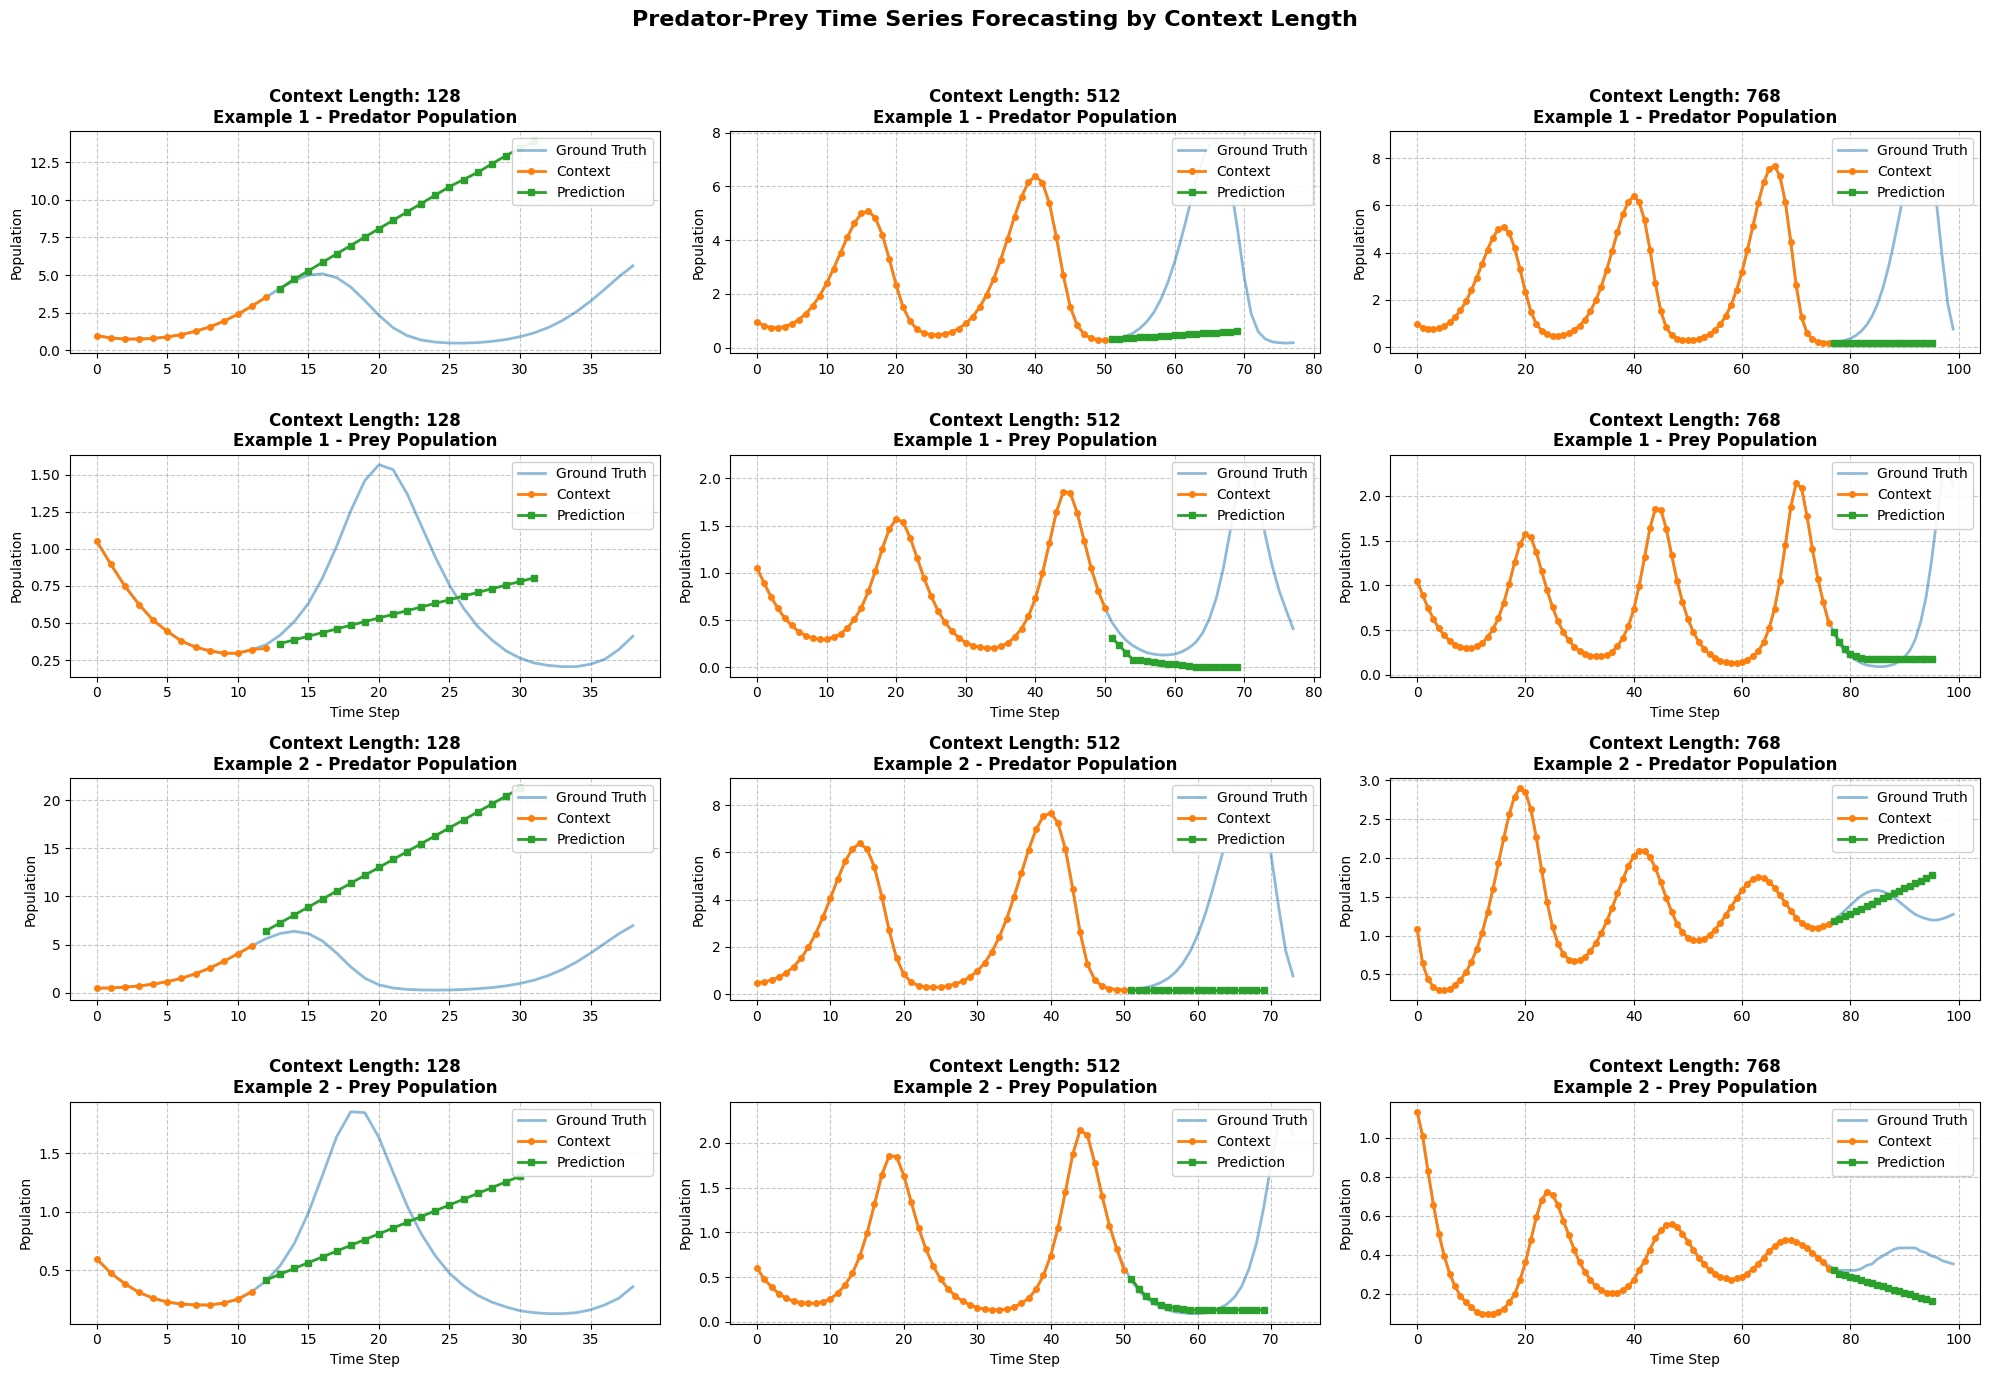
\includegraphics[width=0.9\linewidth]{M2 Course Work//Images/untrained_performance.png} % Adjusted width slightly
    \caption{Visualization of the untrained \texttt{Qwen} model's predictions (red lines) for the next 20 time steps compared to the ground truth (blue/orange lines) on selected test samples. The model fails to capture the underlying dynamics, often predicting constant values.}
    \label{fig:untrained_predictions} % Unique descriptive label
\end{figure}

\subsection{Initial Training with Default Hyperparameters}

Following the baseline evaluation, the model was fine-tuned for 1000 optimizer steps using the default hyper-parameters provided in the LoRA skeleton code (Context Length $S=512$, Learning Rate $\eta=10^{-4}$, LoRA Rank $r=4$). The training and validation loss curves, presented in Figure \ref{fig:initial_loss_curves}, show a consistent decrease, indicating successful learning during this initial phase.

\begin{figure}[!htbp] 
    \centering 
    \begin{subfigure}[b]{0.48\linewidth} 
        \centering
        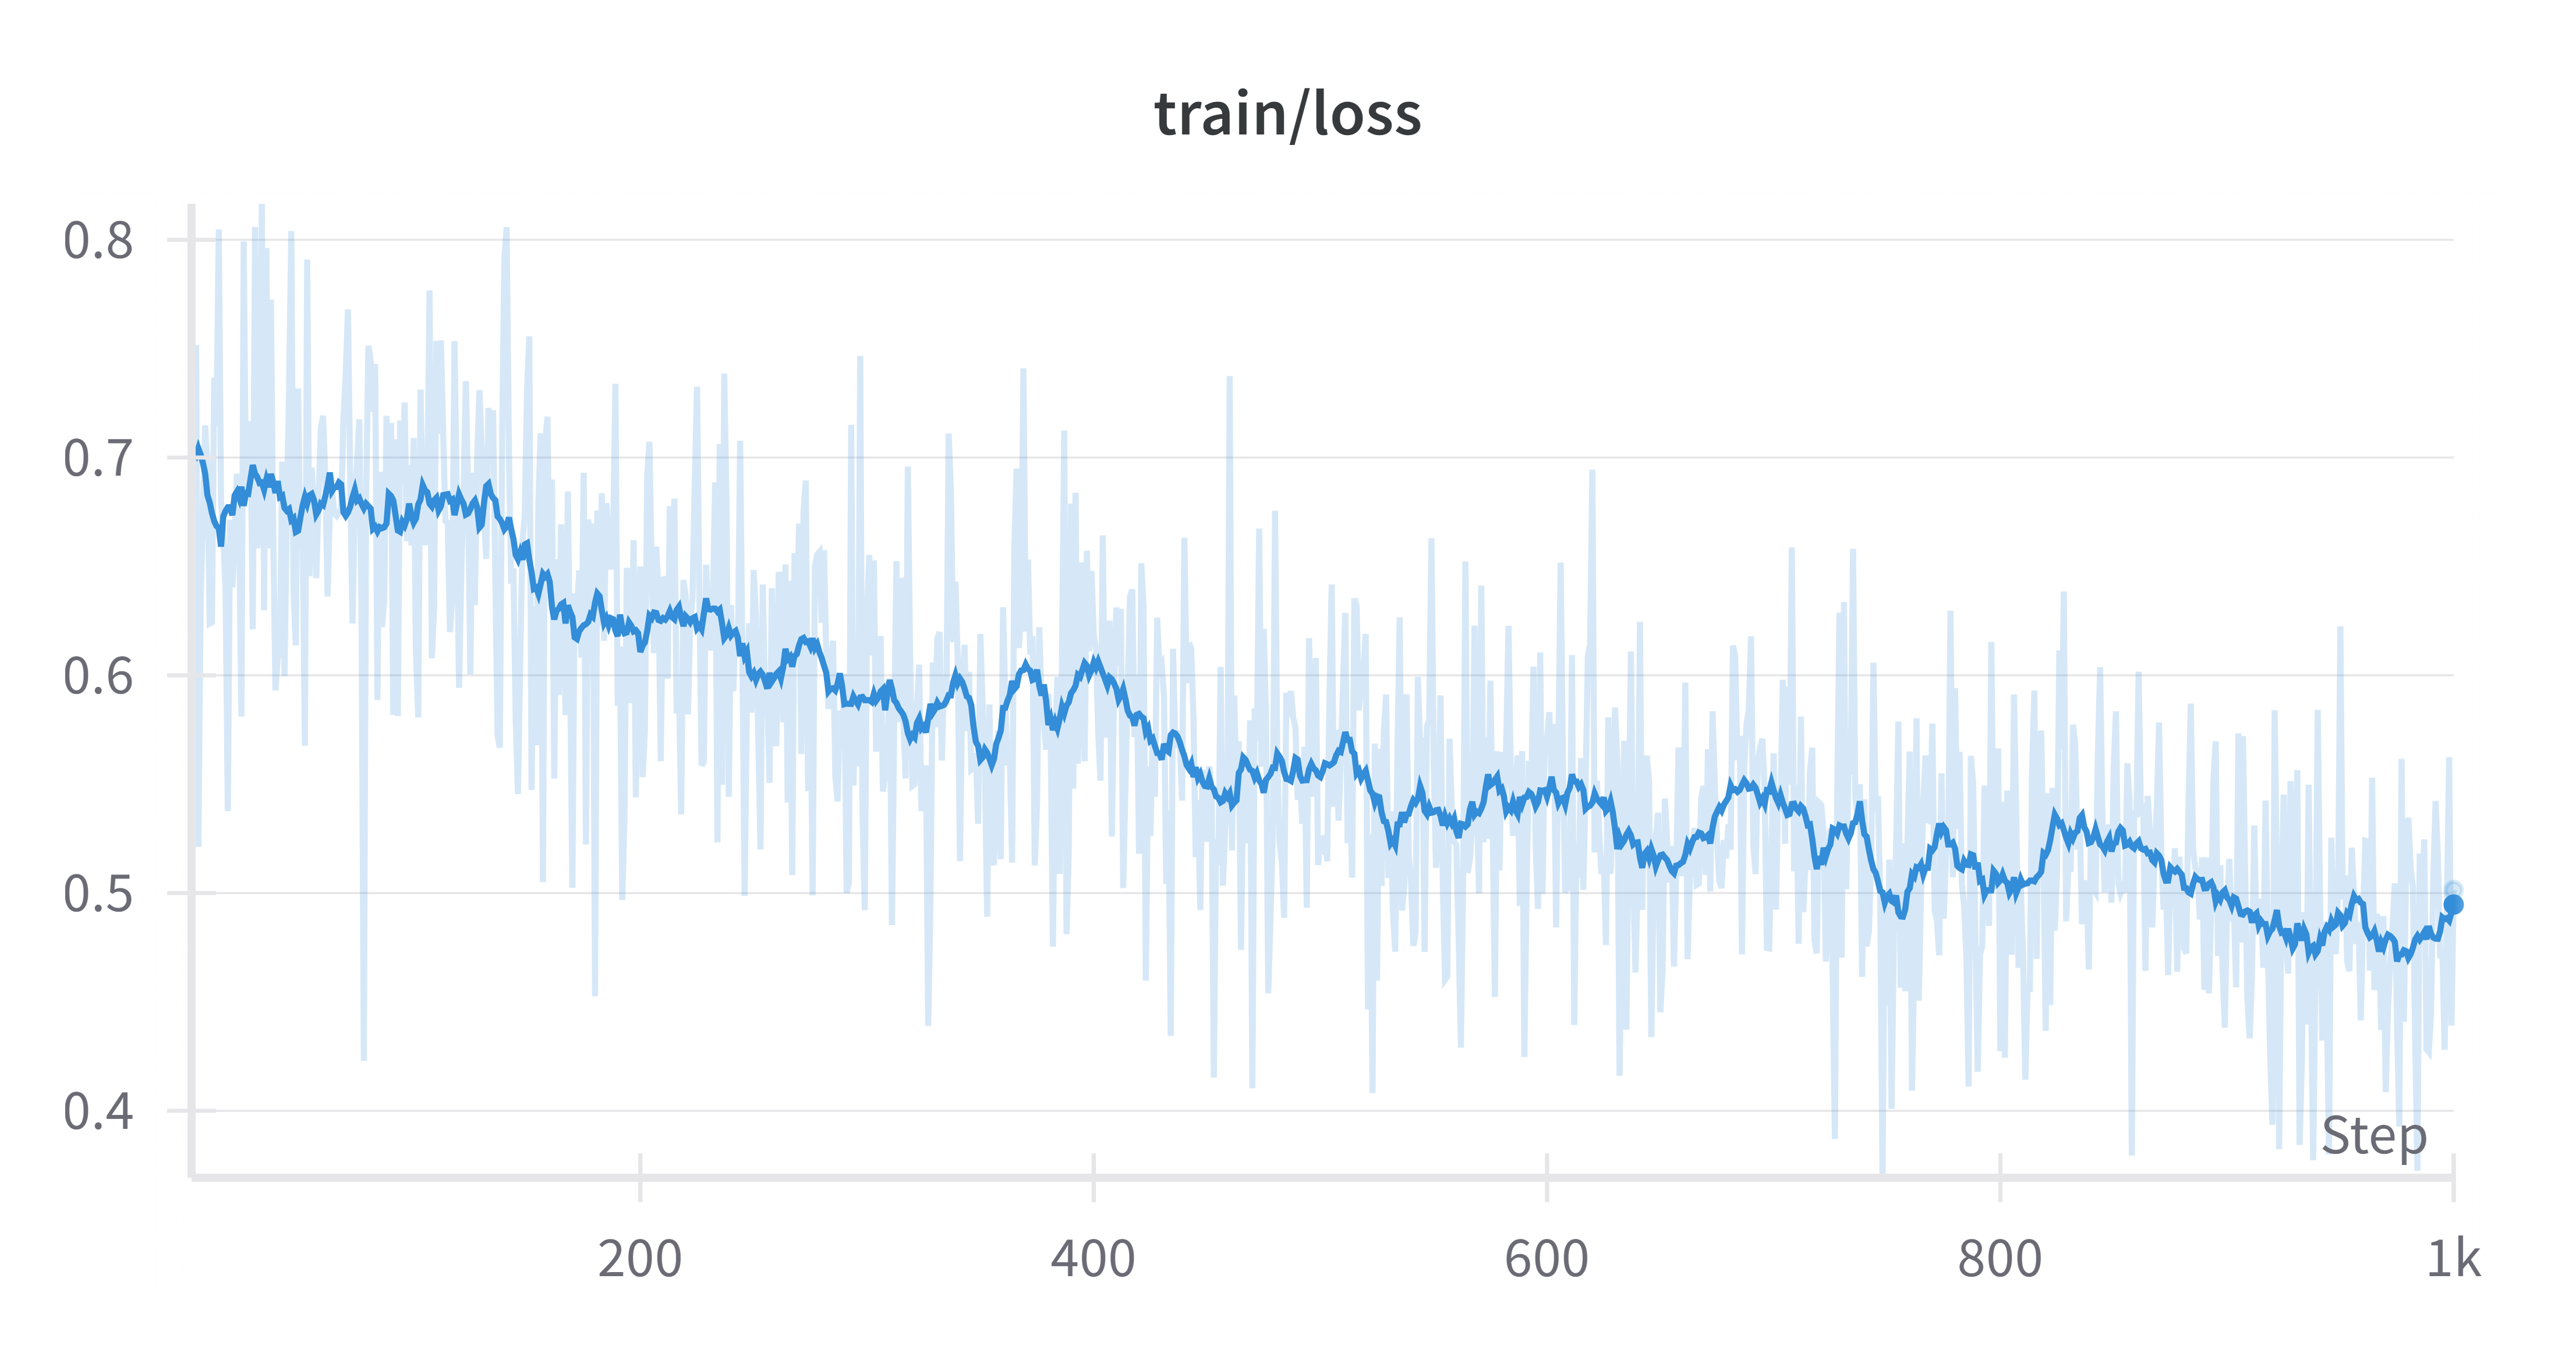
\includegraphics[width=\linewidth]{M2 Course Work//Images/initial_train_loss.png}
        \caption{Training Loss} % Added subcaption
        \label{fig:initial_train_loss} % Unique subfigure label
    \end{subfigure}
    \hfill 
    \begin{subfigure}[b]{0.48\linewidth}
        \centering
        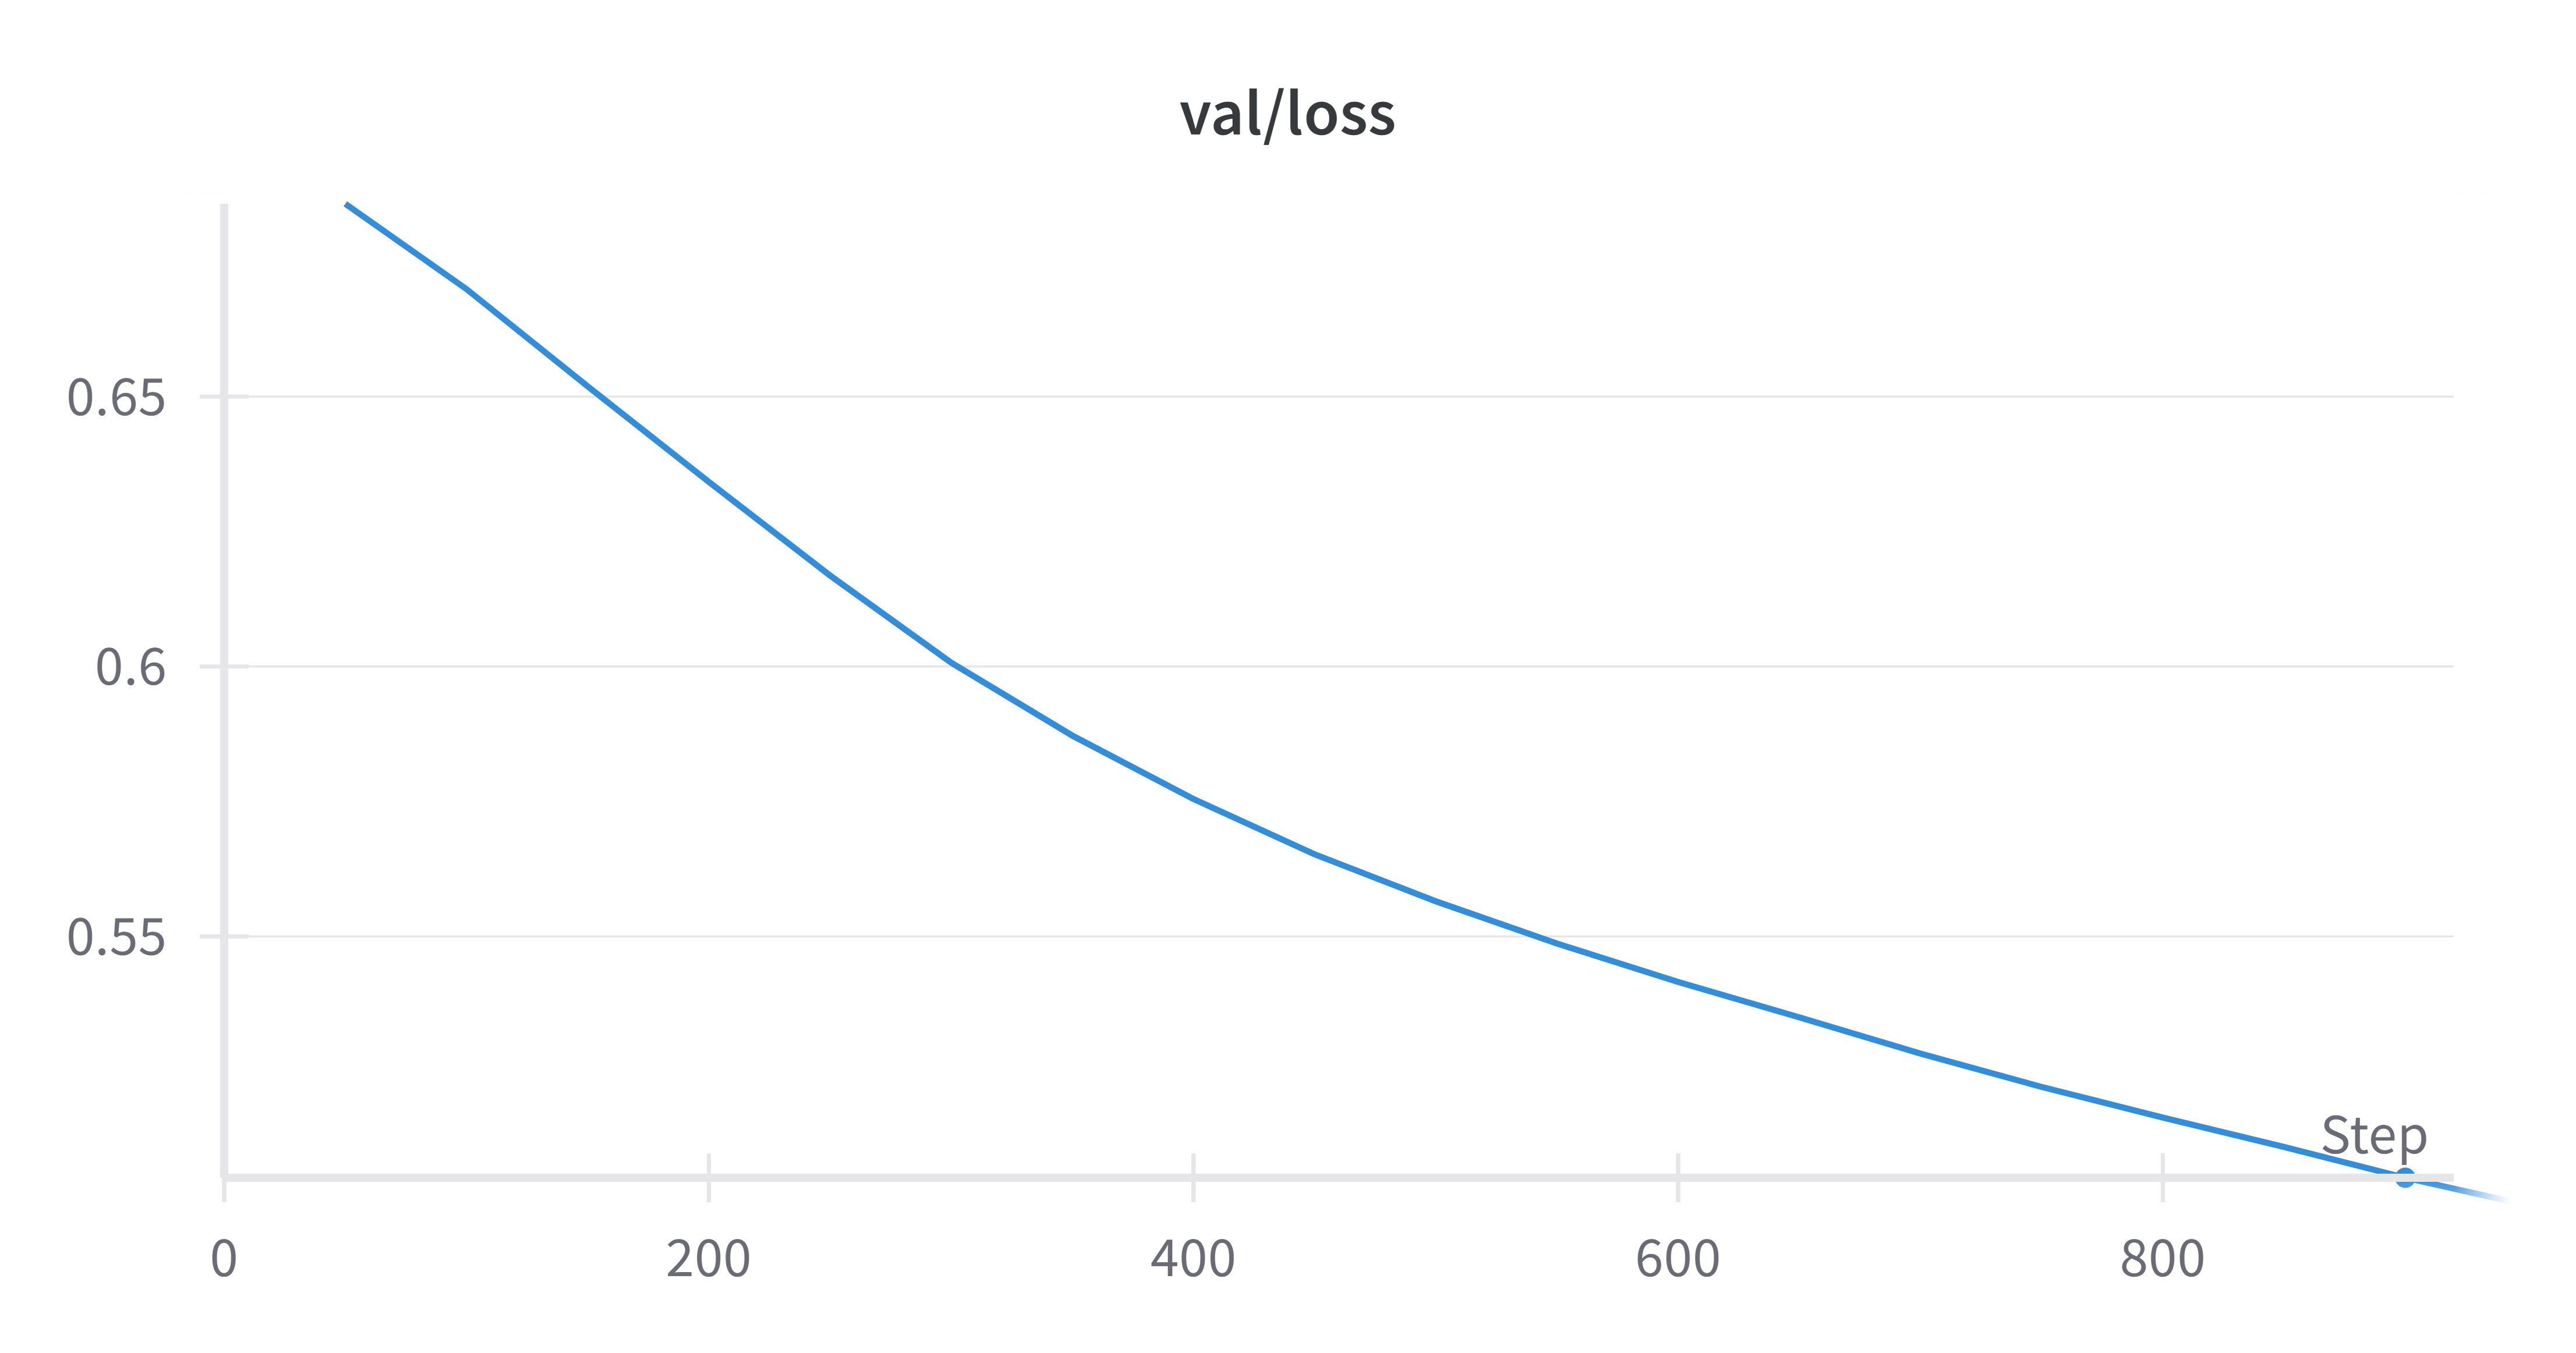
\includegraphics[width=\linewidth]{M2 Course Work//Images/initial_validation_loss.png}
        \caption{Validation Loss} % Added subcaption
        \label{fig:initial_valid_loss} % Unique subfigure label
    \end{subfigure}
    \caption{Training and validation loss curves during the initial 1000 steps of fine-tuning with default hyperparameters.}
    \label{fig:initial_loss_curves} % Unique label for the figure
\end{figure}

Performance metrics on the test set after this initial training are shown in the Initial Training section of Table \ref{tab:training_stage_comparison}. A significant improvement over the untrained baseline is evident, with MSE and MAE values reduced by approximately an order of magnitude for the $S=512$ case it was trained on.

\begin{table}[!htbp] % Use htbp
\renewcommand{\arraystretch}{1.4}
\centering
\setlength{\tabcolsep}{8pt} 
\begin{tabular}{crr}
    \toprule
    \textbf{Context Length ($S$)} & \textbf{MSE} & \textbf{MAE} \\
    \midrule
    128 & 0.135554 & 0.174634 \\
    512 & 0.036210 & 0.083372 \\
    768 & 0.029675 & 0.065142 \\
    \bottomrule
\end{tabular}
\caption{Test set performance after 1000 steps of initial training ($S=512, \eta=10^{-4}, r=4$).} 
\label{tab:initial_training_metrics} 
\end{table}

Interestingly, the model also demonstrates improved performance when evaluated on context lengths different from the one used during training ($S=128$ and $S=768$). 

Visual inspection of predictions (Figure \ref{fig:initial_training_predictions}) confirms this progress. The model no longer predicts straight lines; instead, it generates outputs with curved structures that attempt to follow the cyclical patterns, although they may deviate in amplitude or phase and sometimes regress towards simpler patterns over longer horizons. This represents a substantial improvement over the baseline, demonstrating the potential of fine-tuning LLMs for this task using the adopted sequence representation.

\begin{figure}[!htbp] % Use htbp
    \centering
    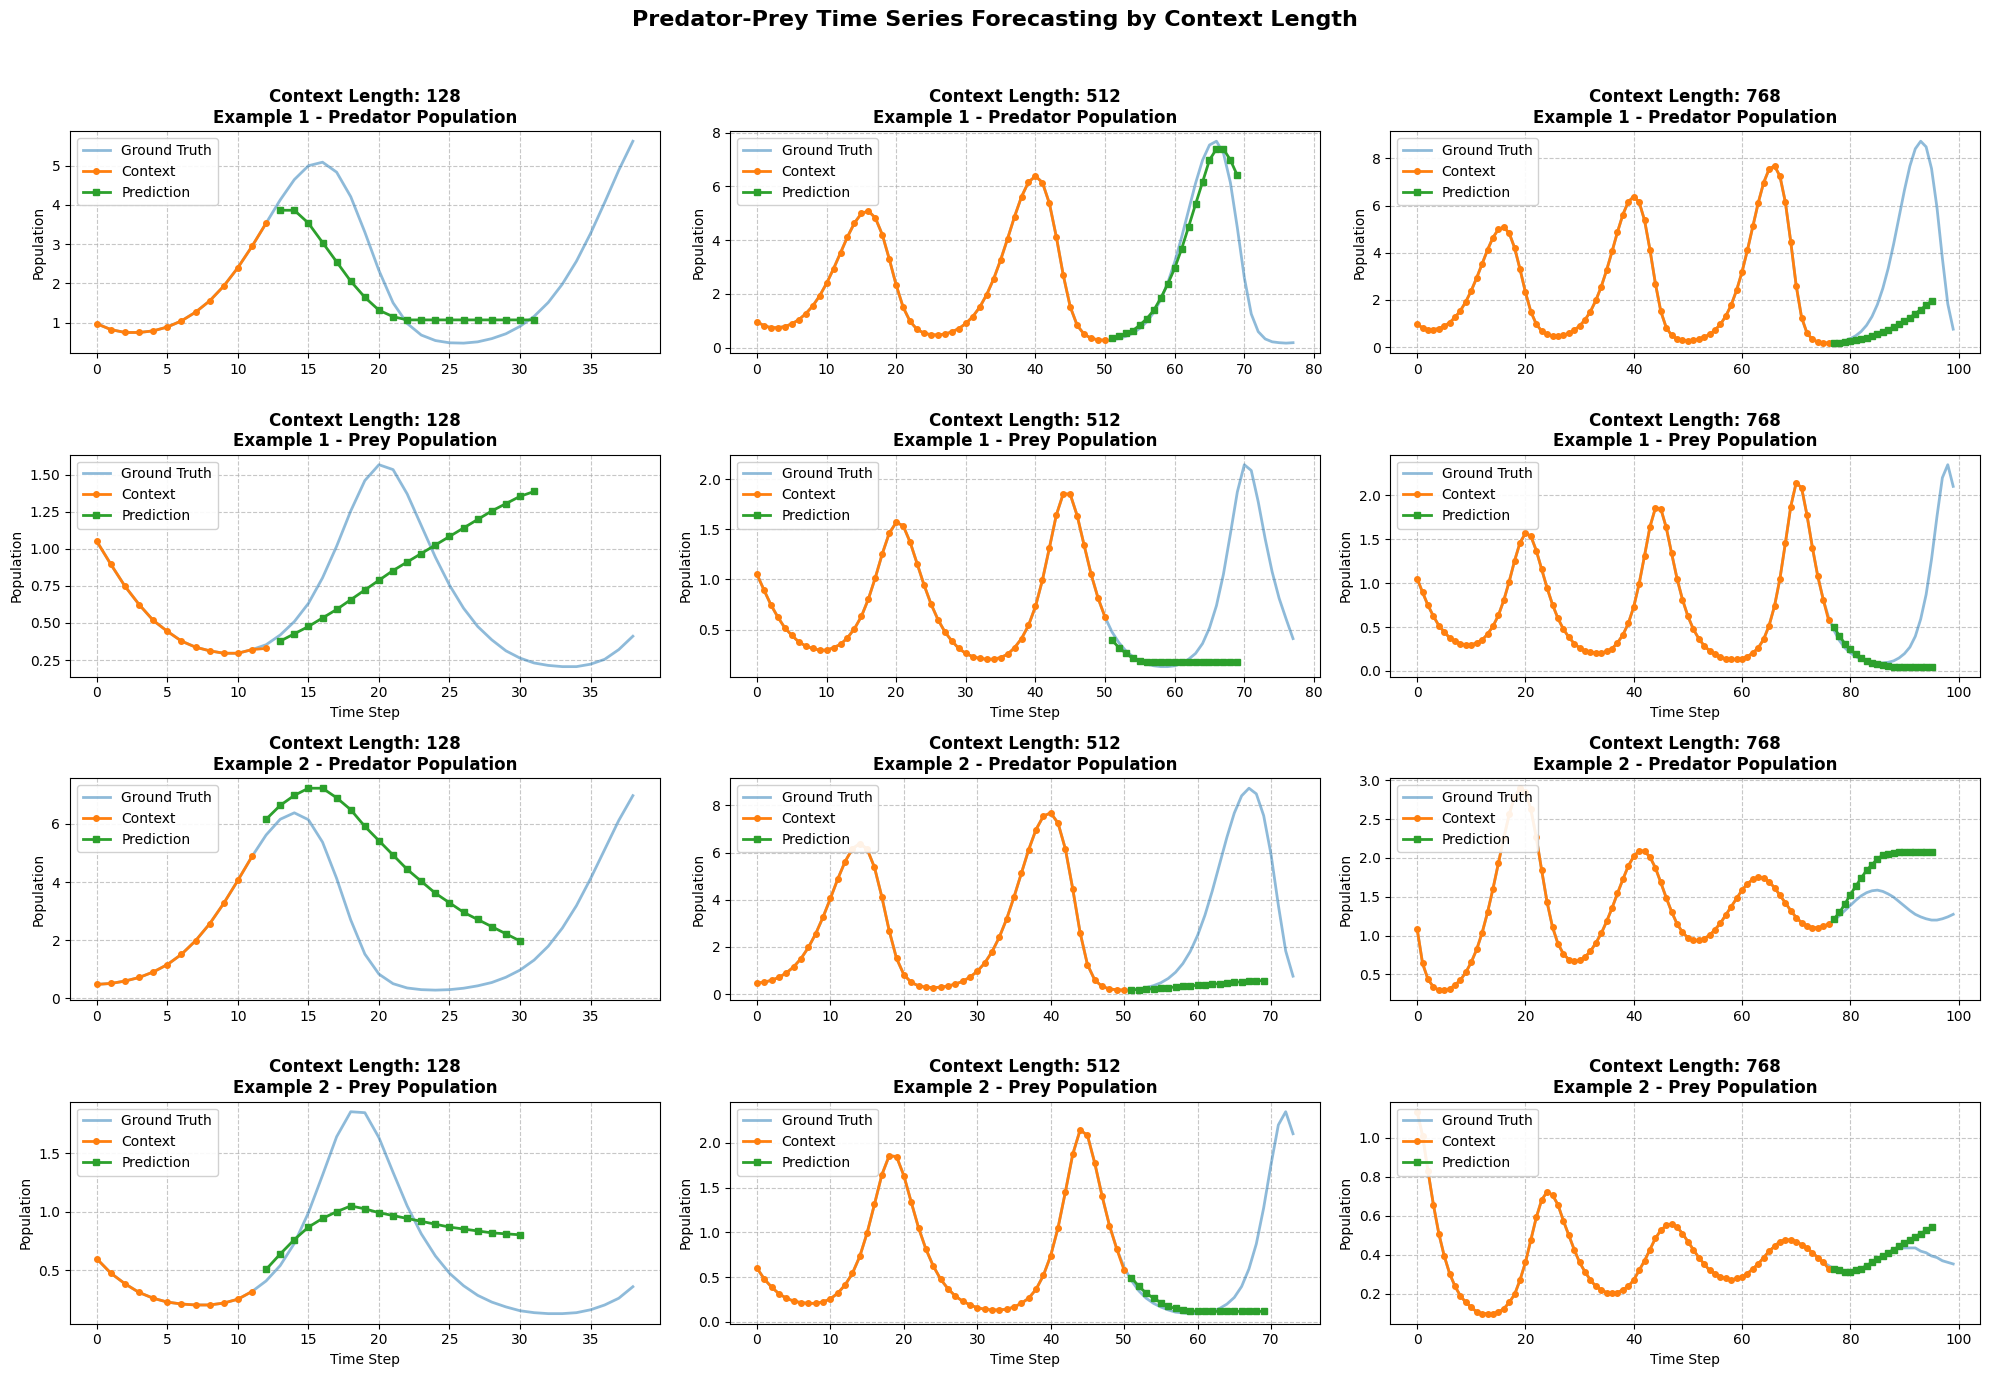
\includegraphics[width=0.9\linewidth]{M2 Course Work//Images/intial_training_result.png} % Adjusted width
    \caption{Visualization of model predictions after initial training (1000 steps). Compared to Figure \ref{fig:untrained_predictions}, the model now attempts to capture the cyclical dynamics, producing curved trajectories instead of constant values.}
    \label{fig:initial_training_predictions} % Unique label
\end{figure}

\subsection{Grid Search over Learning Rate and LoRA Rank}

To optimize performance, we conducted a grid search over the learning rate ($\eta \in \{10^{-4}, 5 \times 10^{-5}, 10^{-5}\}$) and LoRA rank ($r \in \{2, 4, 8\}$), keeping the context length fixed at $S=512$. Each combination was trained for 500 steps, using the \texttt{wandb.sweep} functionality for experiment management. The training and validation loss curves for these runs (aggregated view in Figure \ref{fig:grid_search_lr_rank_loss_curves}) generally showed decreasing trends, as expected.

\begin{figure}[!htbp] 
    \centering 
    \begin{subfigure}[b]{0.48\linewidth} 
        \centering
        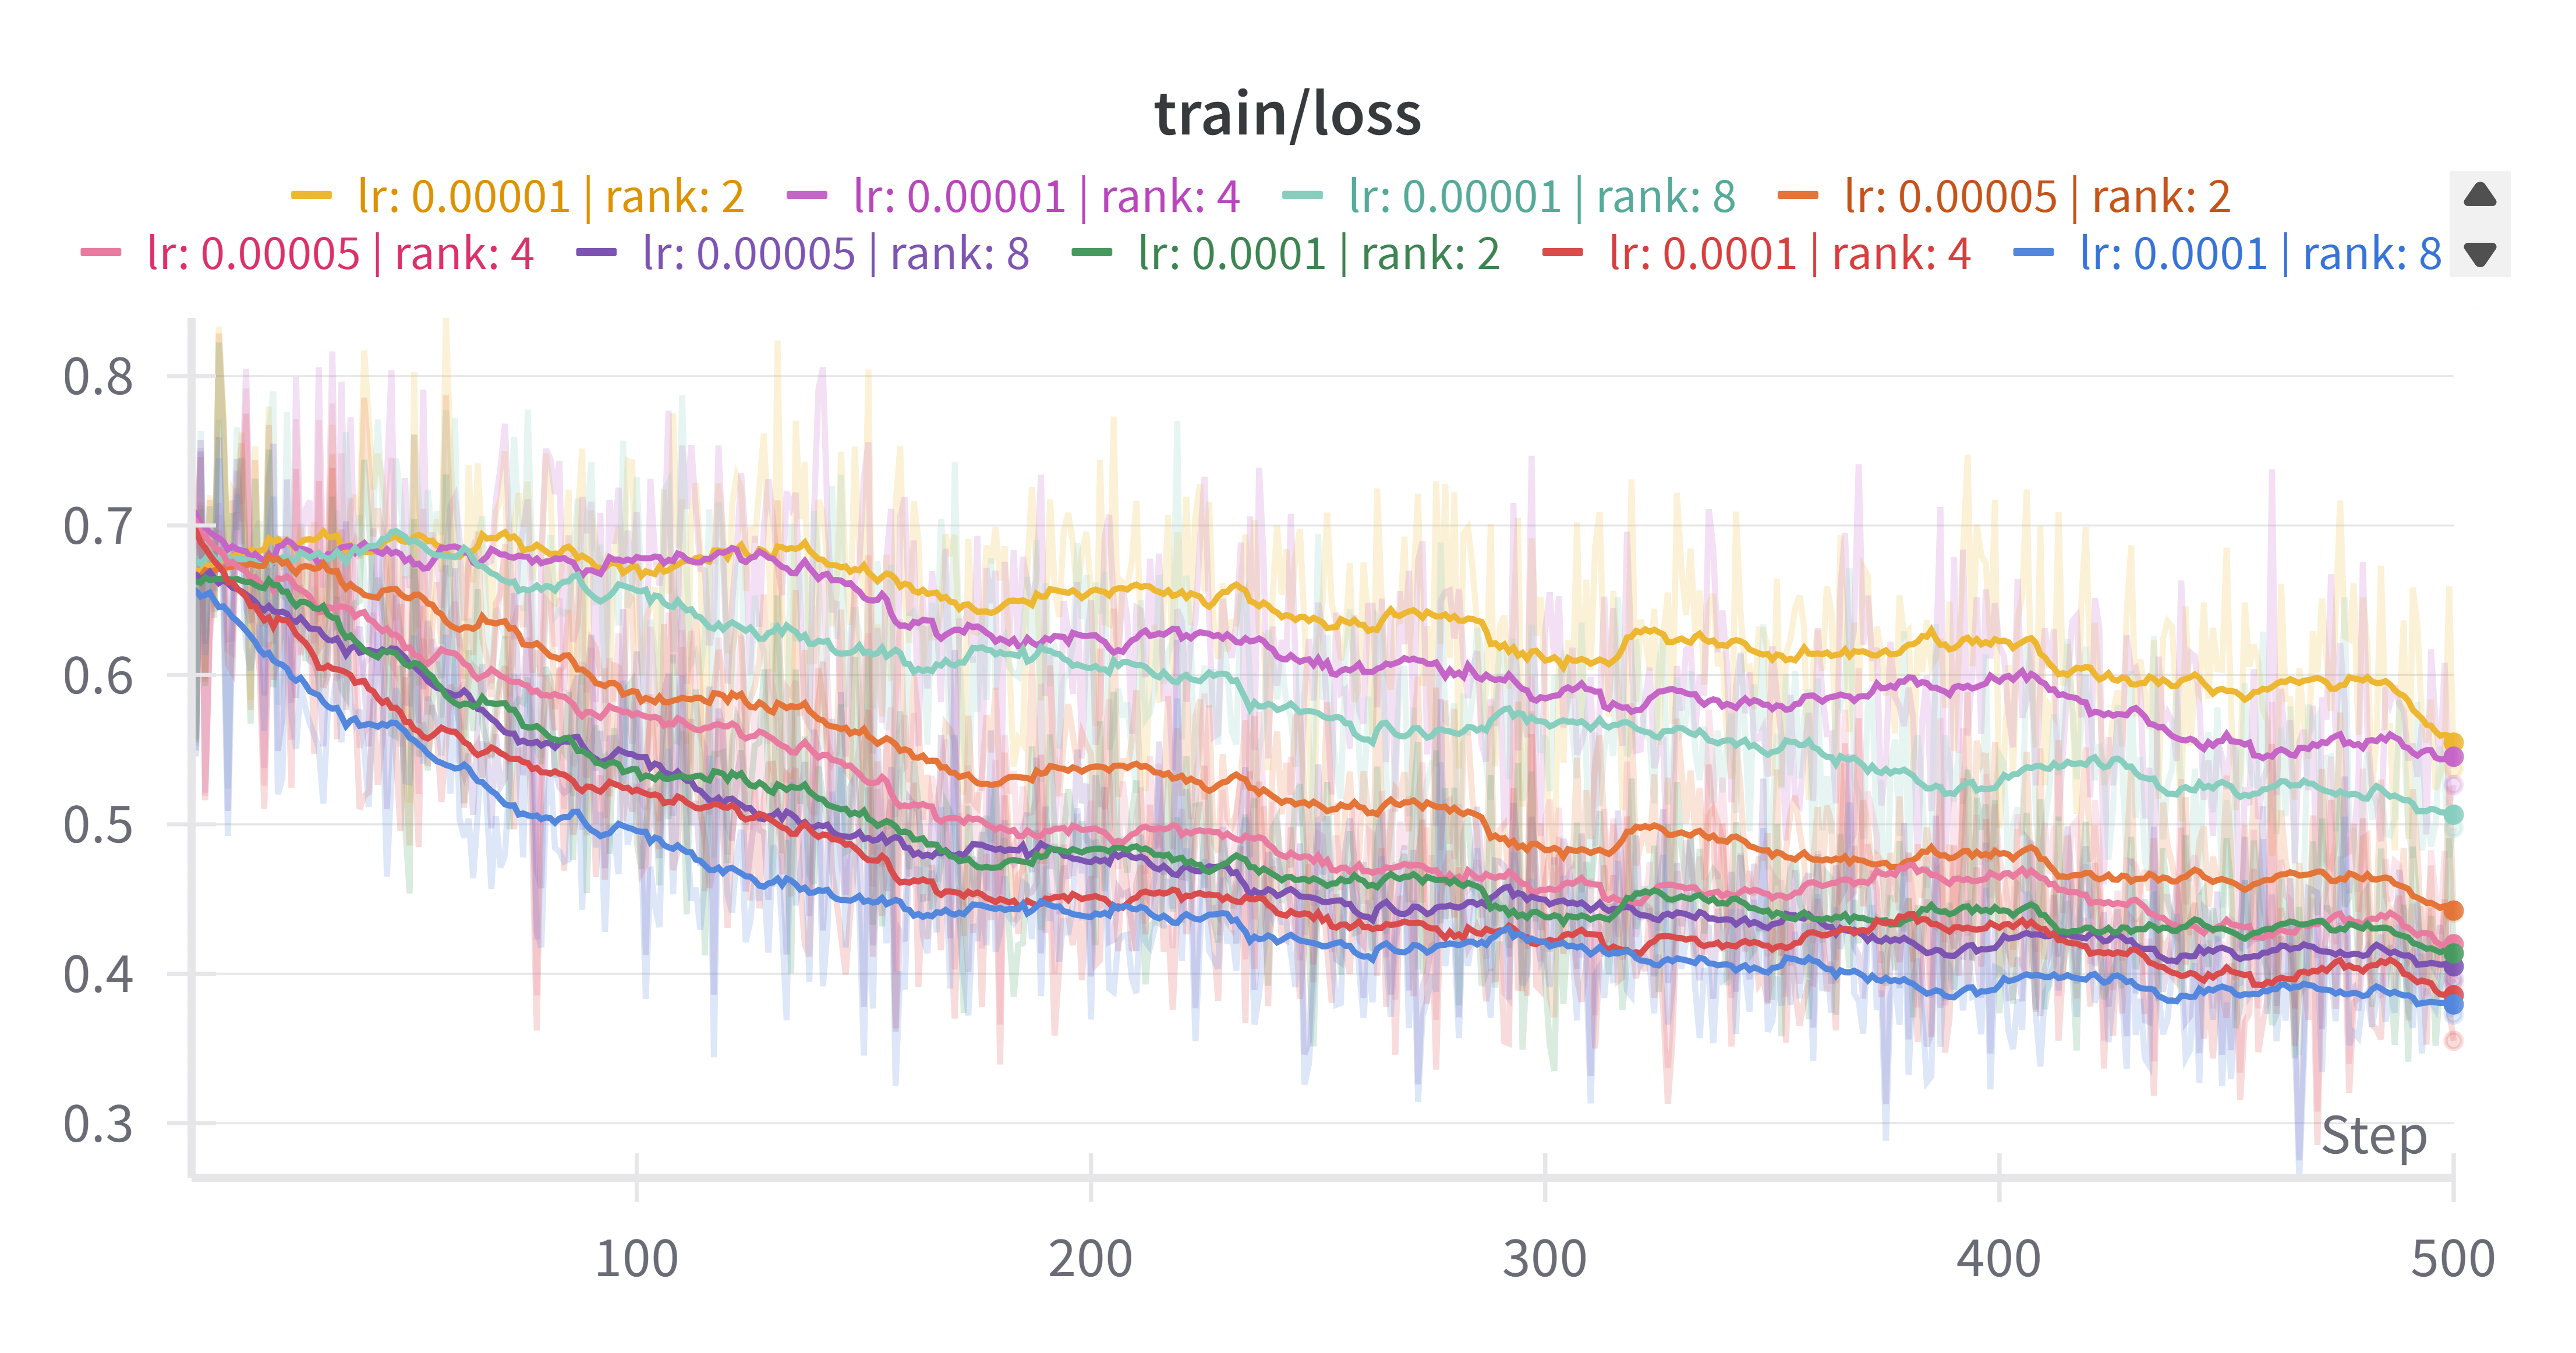
\includegraphics[width=\linewidth]{M2 Course Work//Images/grid_search_training_loss.png}
        \caption{Training Loss (All Runs)} % Added subcaption
        \label{fig:grid_search_lr_rank_train_loss} % Unique subfigure label
    \end{subfigure}
    \hfill 
    \begin{subfigure}[b]{0.48\linewidth}
        \centering
        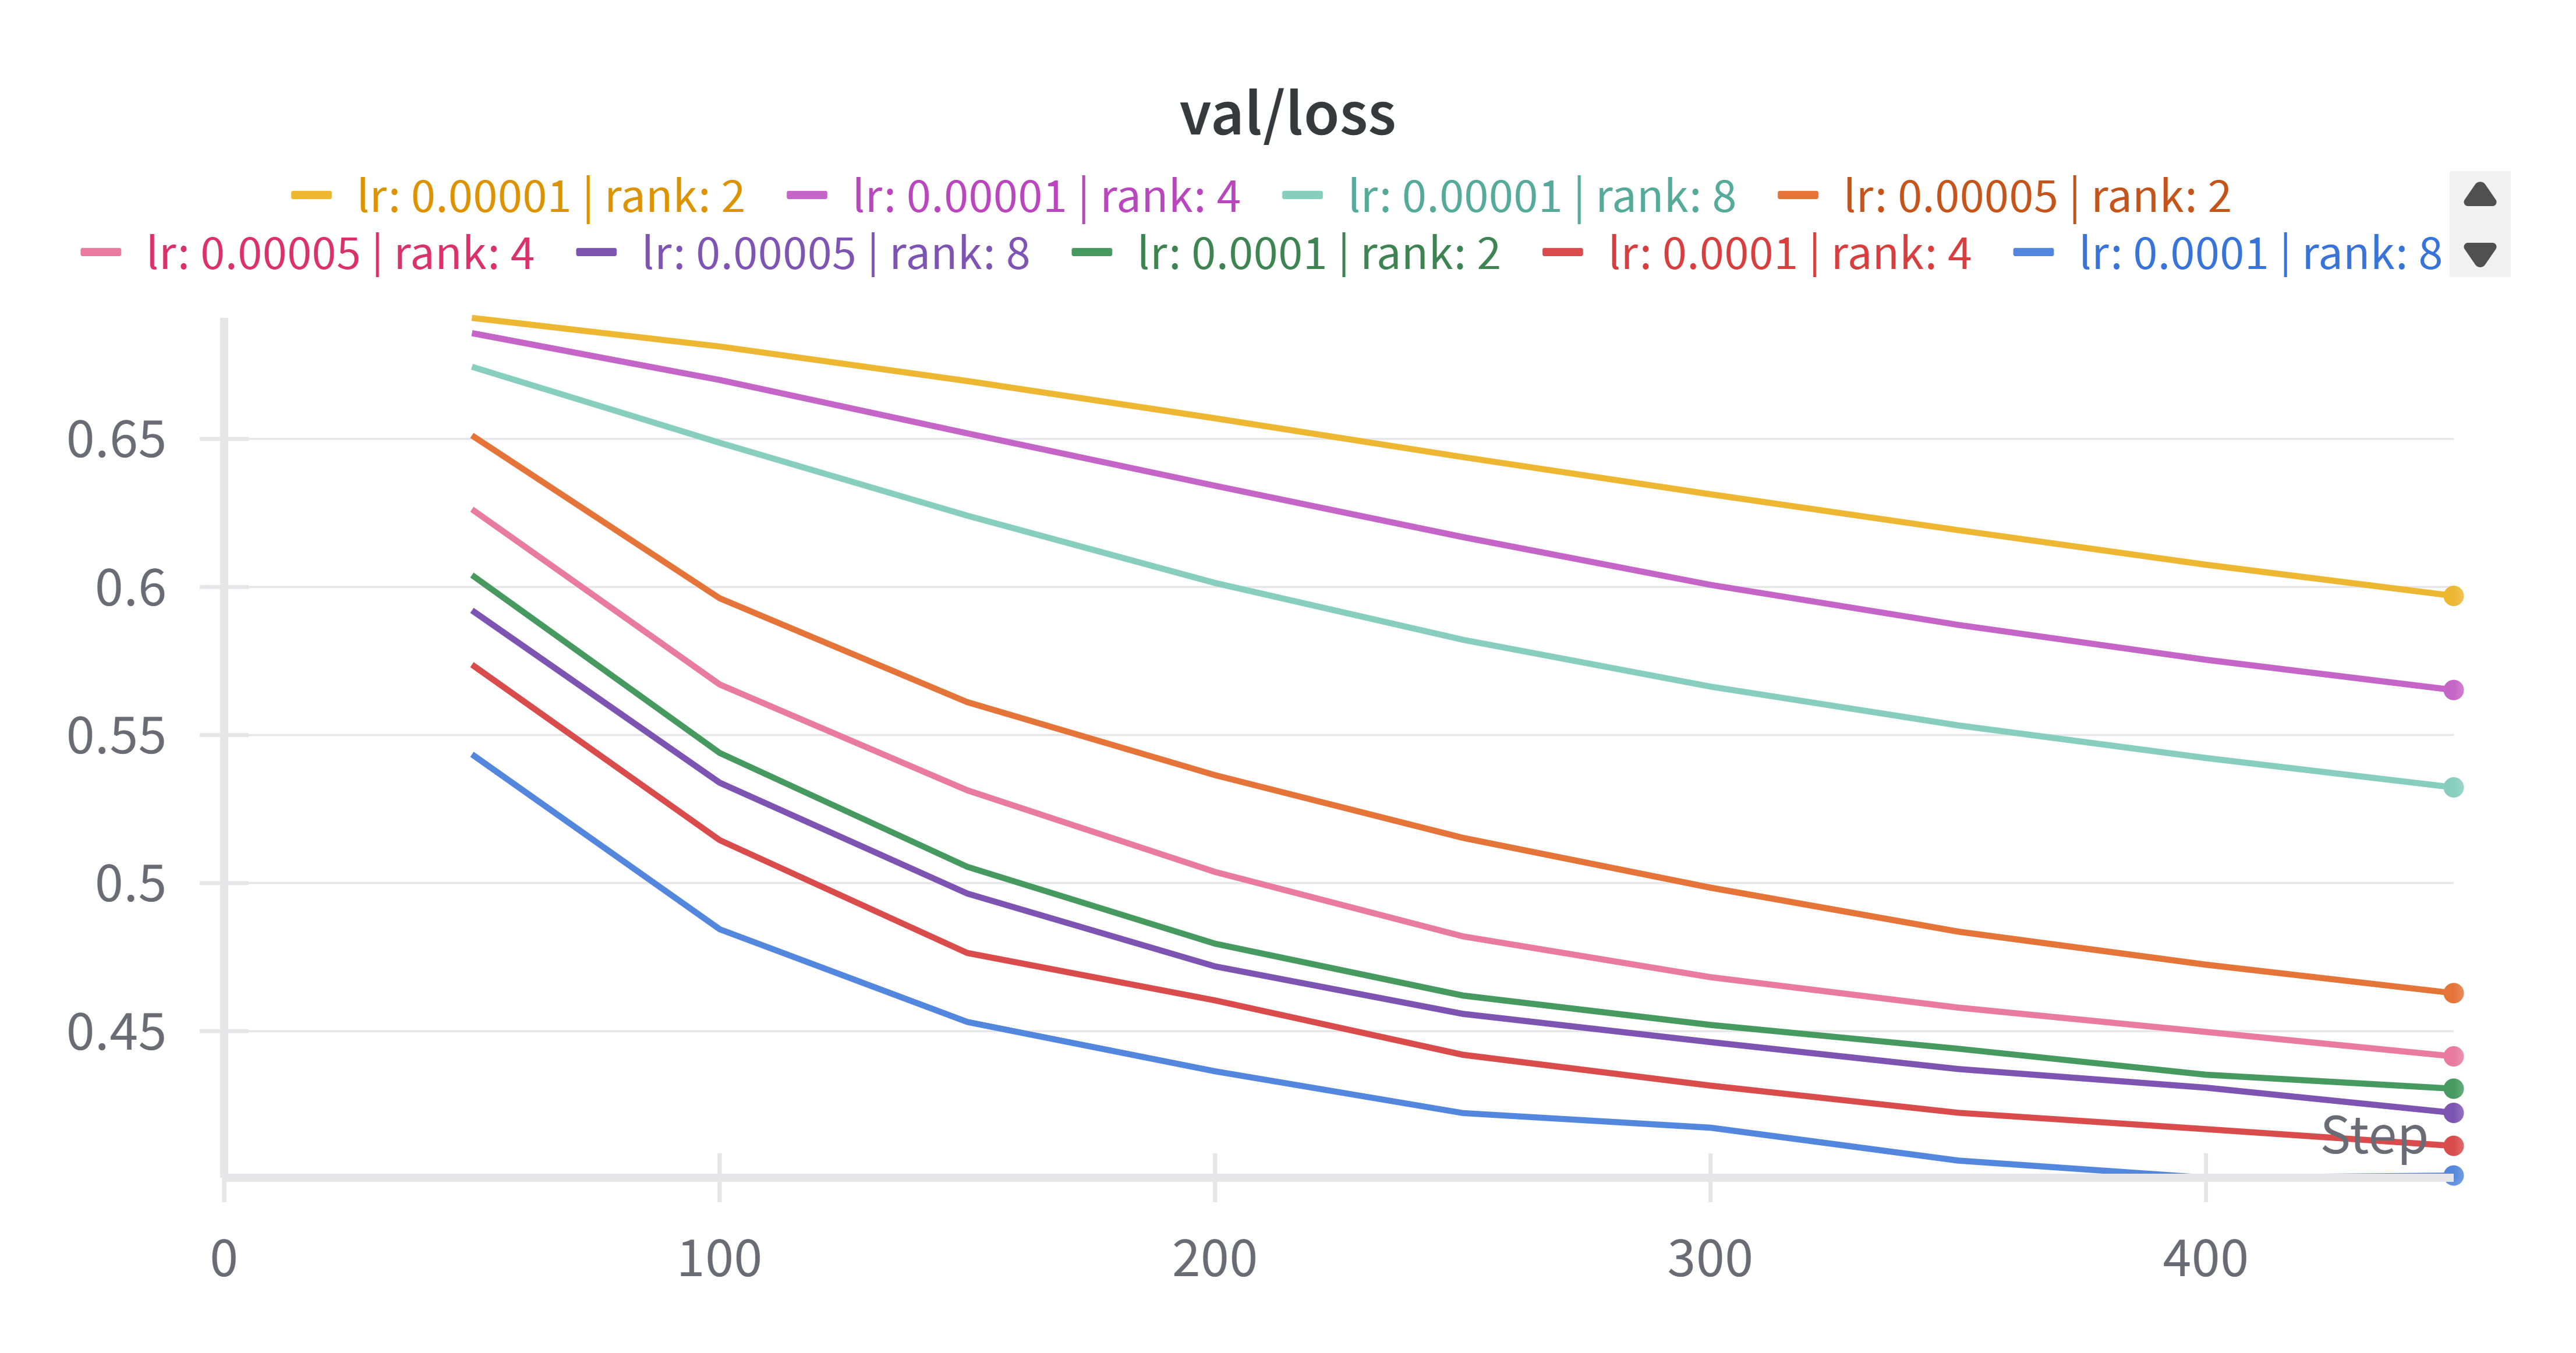
\includegraphics[width=\linewidth]{M2 Course Work//Images/grid_search_validiation_loss.png}
        \caption{Validation Loss (All Runs)} % Added subcaption
        \label{fig:grid_search_lr_rank_valid_loss} % Unique subfigure label
    \end{subfigure}
    \caption{Training and validation loss curves (combined view) from the grid search over learning rate and LoRA rank.}
    \label{fig:grid_search_lr_rank_loss_curves} % Unique label for the figure
\end{figure}

The primary metric for comparison was the final validation MAE after 500 steps for each run, summarized visually in Figure \ref{fig:grid_search_lr_rank_results}.

\begin{figure}[!htbp] 
    \centering
    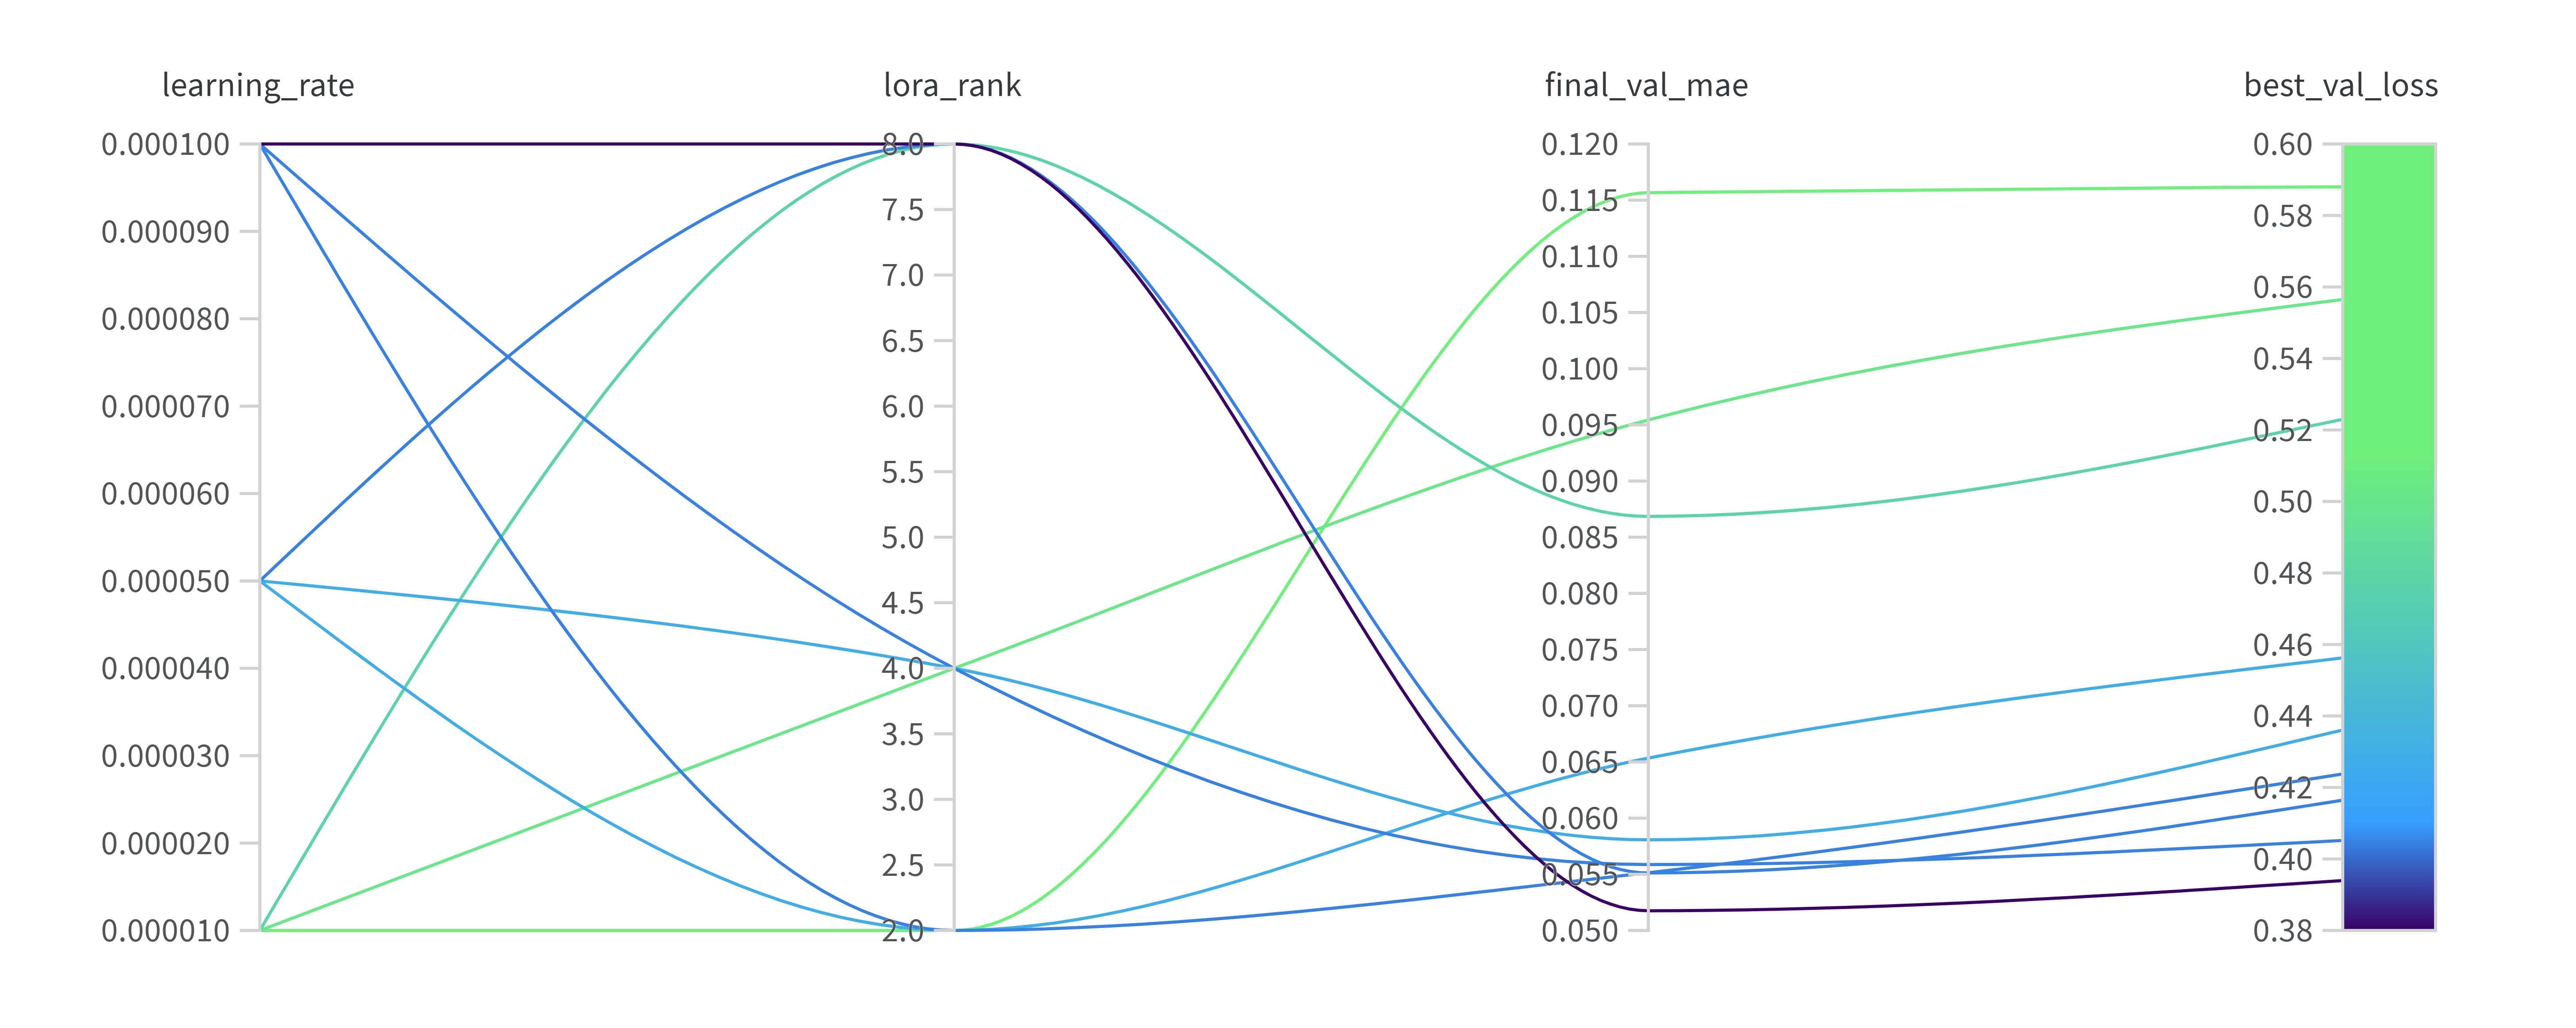
\includegraphics[width=0.8\linewidth]{M2 Course Work//Images/grid_search_result.png}
    \caption{Validation MAE after 500 steps for different combinations of LoRA rank and learning rate (Context Length S=512). Lower MAE indicates better performance.}
    \label{fig:grid_search_lr_rank_results} % Unique label
\end{figure}

The results indicate a clear preference for higher learning rates and higher LoRA ranks within the tested ranges. The best validation MAE was achieved with the highest rank ($r=8$) and the highest learning rate ($\eta=10^{-4}$). This suggests that adapting the \texttt{Qwen} model from its original natural language domain to this specialized numerical time-series task requires significant parameter updates. A higher rank provides more adaptable parameters within the LoRA layers, increasing the model's capacity to learn the new patterns, while a higher learning rate allows for faster convergence towards the new task-specific optimum. Based on this, we selected $\eta=10^{-4}$ and $r=8$ as the preferred parameters for subsequent experiments.

\subsection{Search over Context Length}

Having identified the potentially optimal learning rate and rank, we proceeded to evaluate the impact of context length ($S \in \{128, 512, 768\}$) more formally. We trained separate models for 500 steps each, using the selected $\eta=10^{-4}$ and $r=8$. The loss curves are shown in Figure \ref{fig:context_search_loss_curves}.

\begin{figure}[!htbp] 
    \centering 
    \begin{subfigure}[b]{0.48\linewidth} 
        \centering
        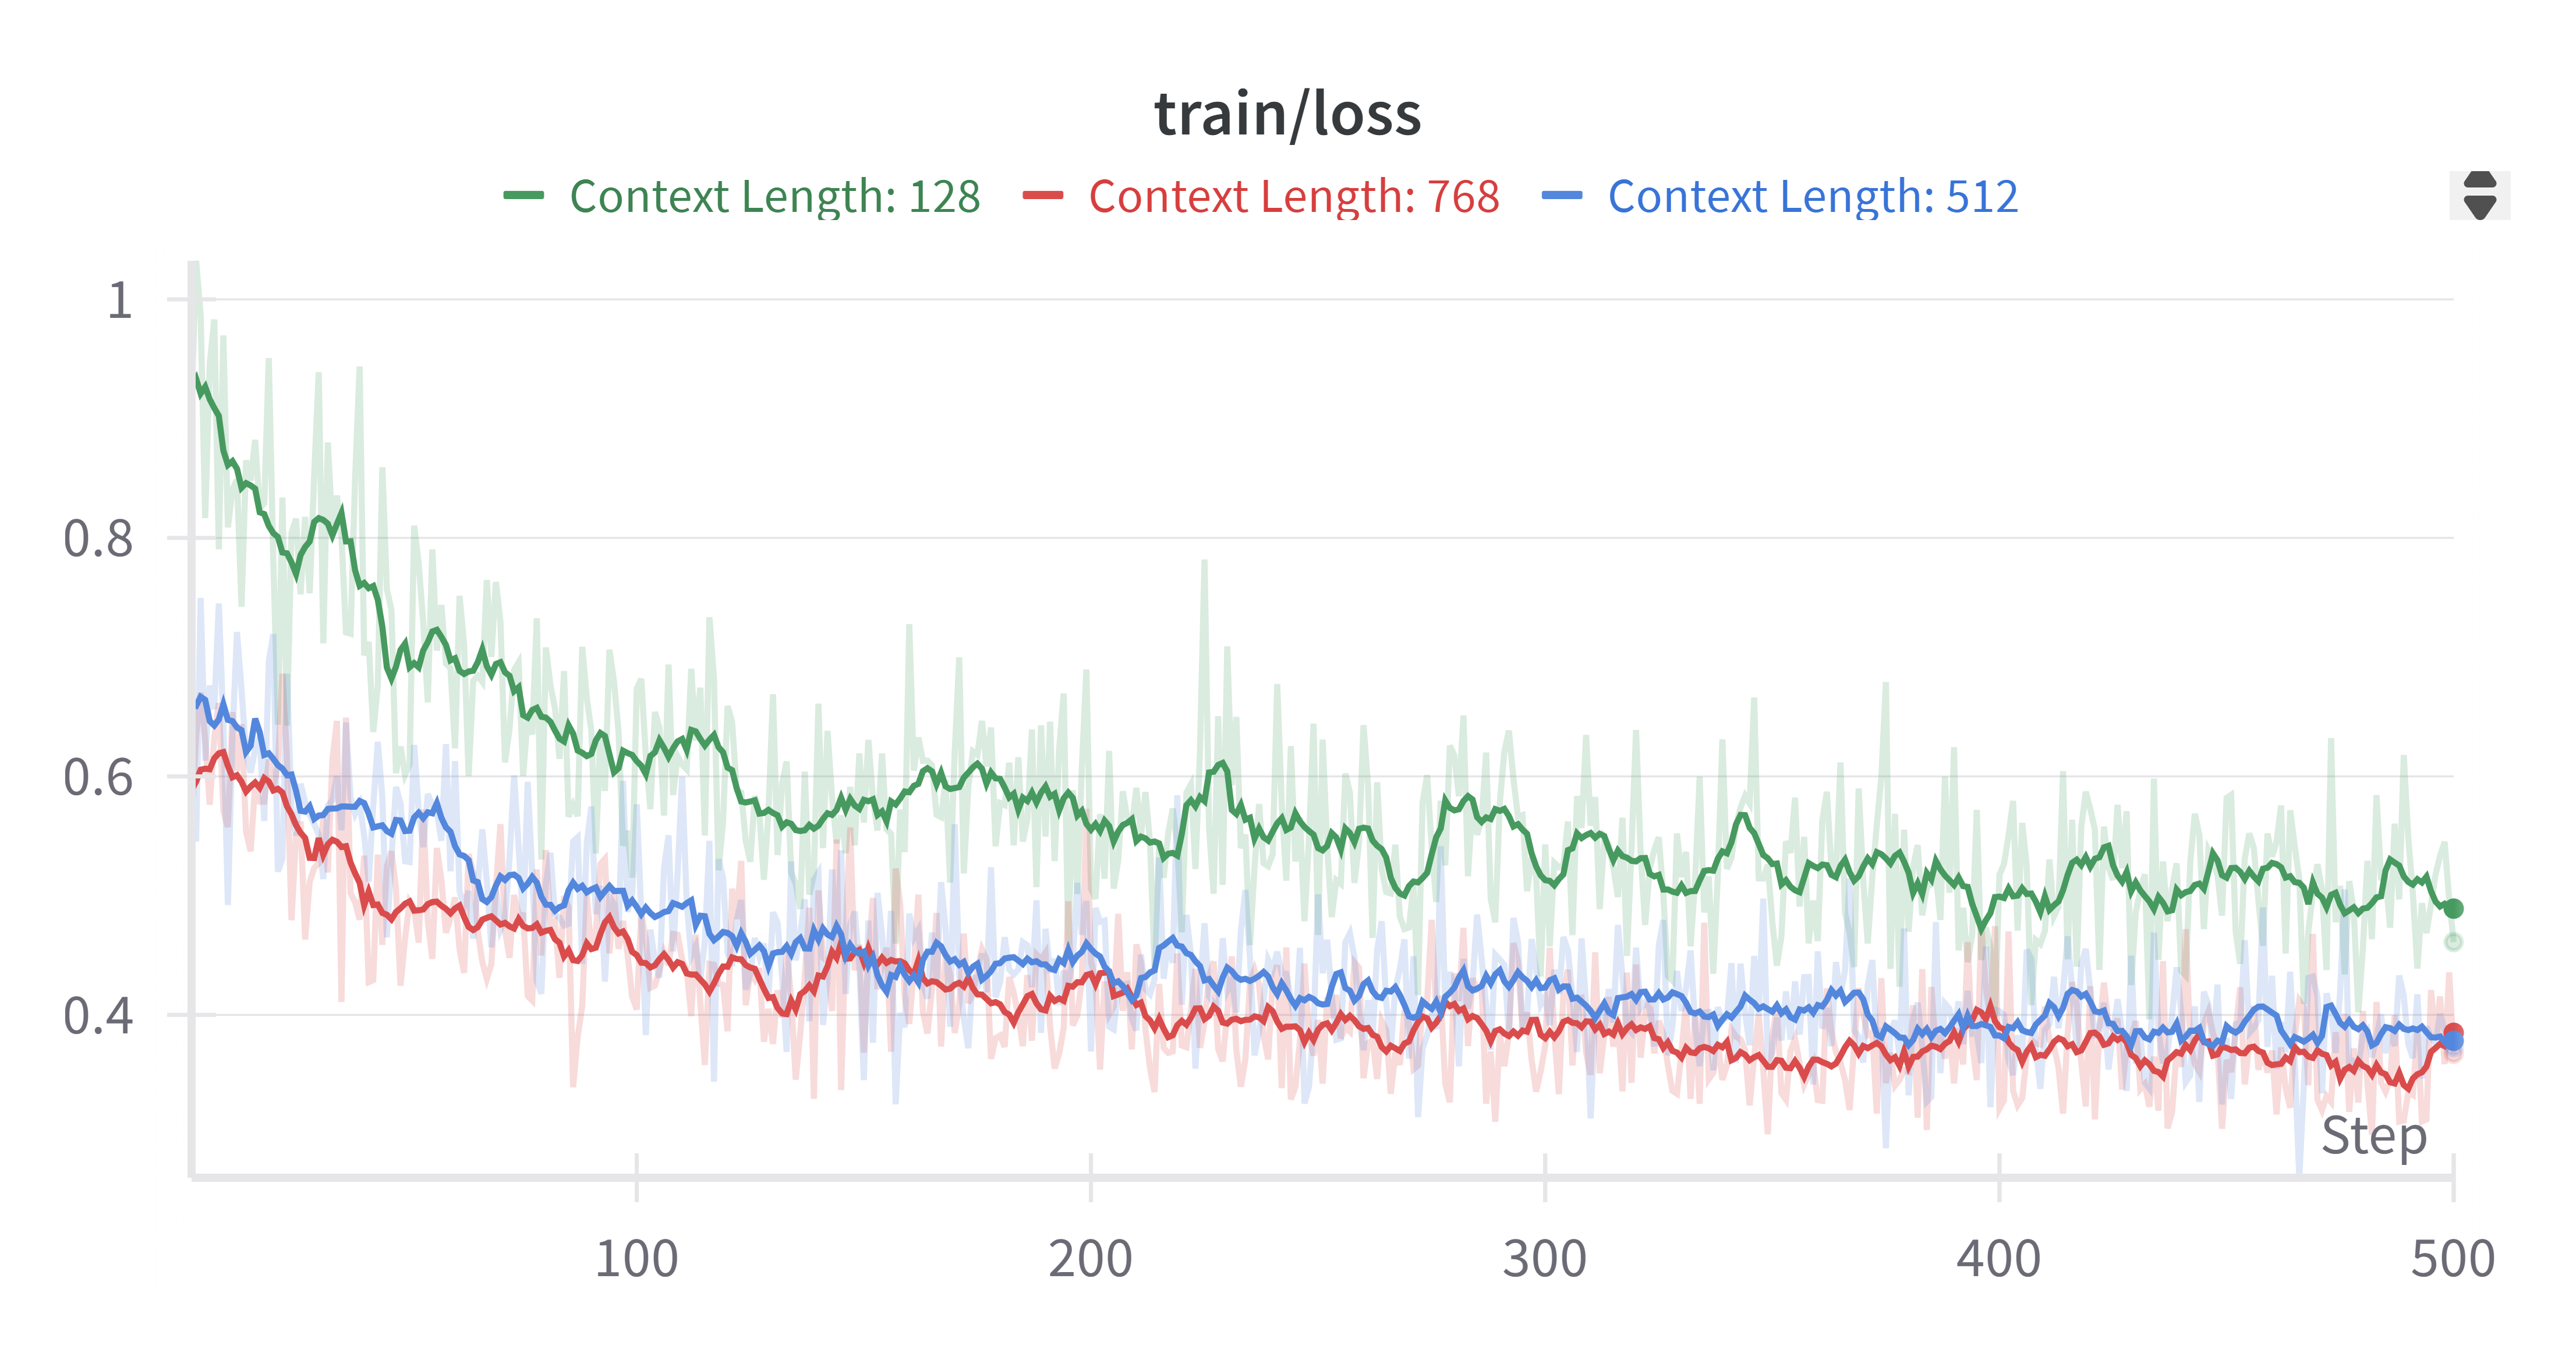
\includegraphics[width=\linewidth]{M2 Course Work/Images/sweep_context_length_training.png}
        \caption{Training Loss} % Added subcaption
        \label{fig:context_search_train_loss} % Unique subfigure label
    \end{subfigure}
    \hfill 
    \begin{subfigure}[b]{0.48\linewidth}
        \centering
        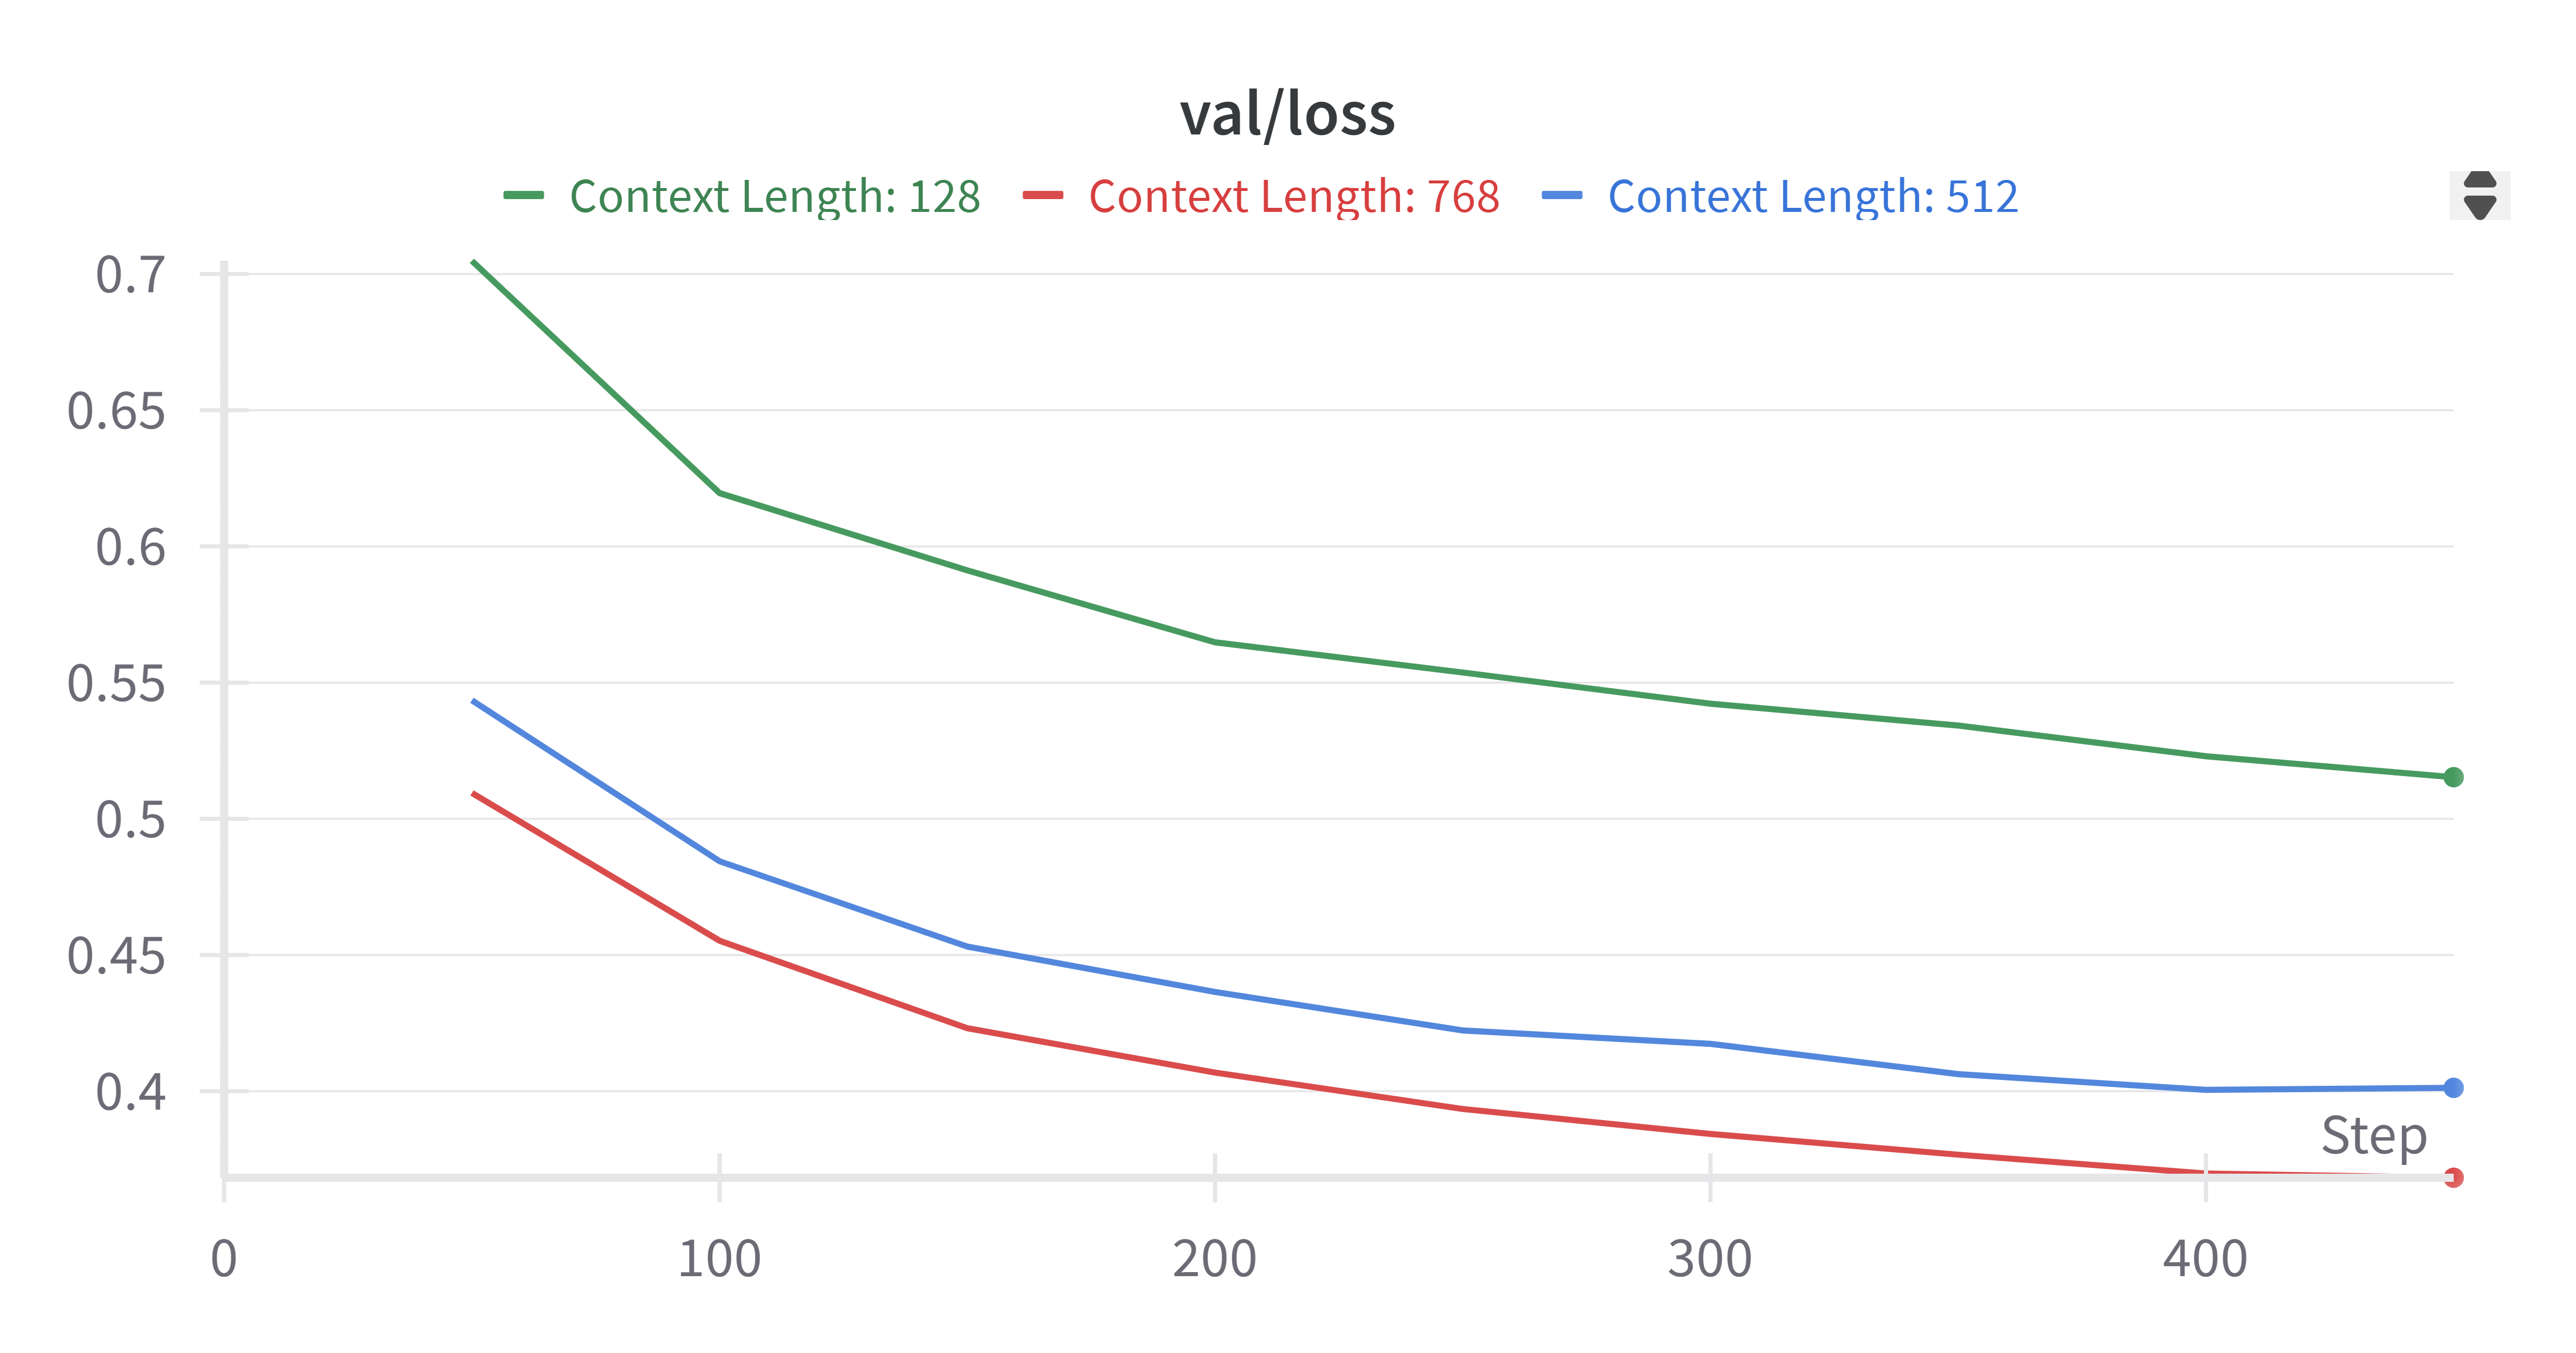
\includegraphics[width=\linewidth]{M2 Course Work/Images/sweep_context_length_validation.png}
        \caption{Validation Loss} % Added subcaption
        \label{fig:context_search_valid_loss} % Unique subfigure label
    \end{subfigure}
    \caption{Training and validation loss curves for models trained with different context lengths ($S \in \{128, 512, 768\}$), using $\eta=10^{-4}, r=8$.}
    \label{fig:context_search_loss_curves} % Unique label for the figure
\end{figure}

The final validation MAE for each context length is compared in Figure \ref{fig:context_search_results}.

\begin{figure}[!htbp] % Use htbp
    \centering
    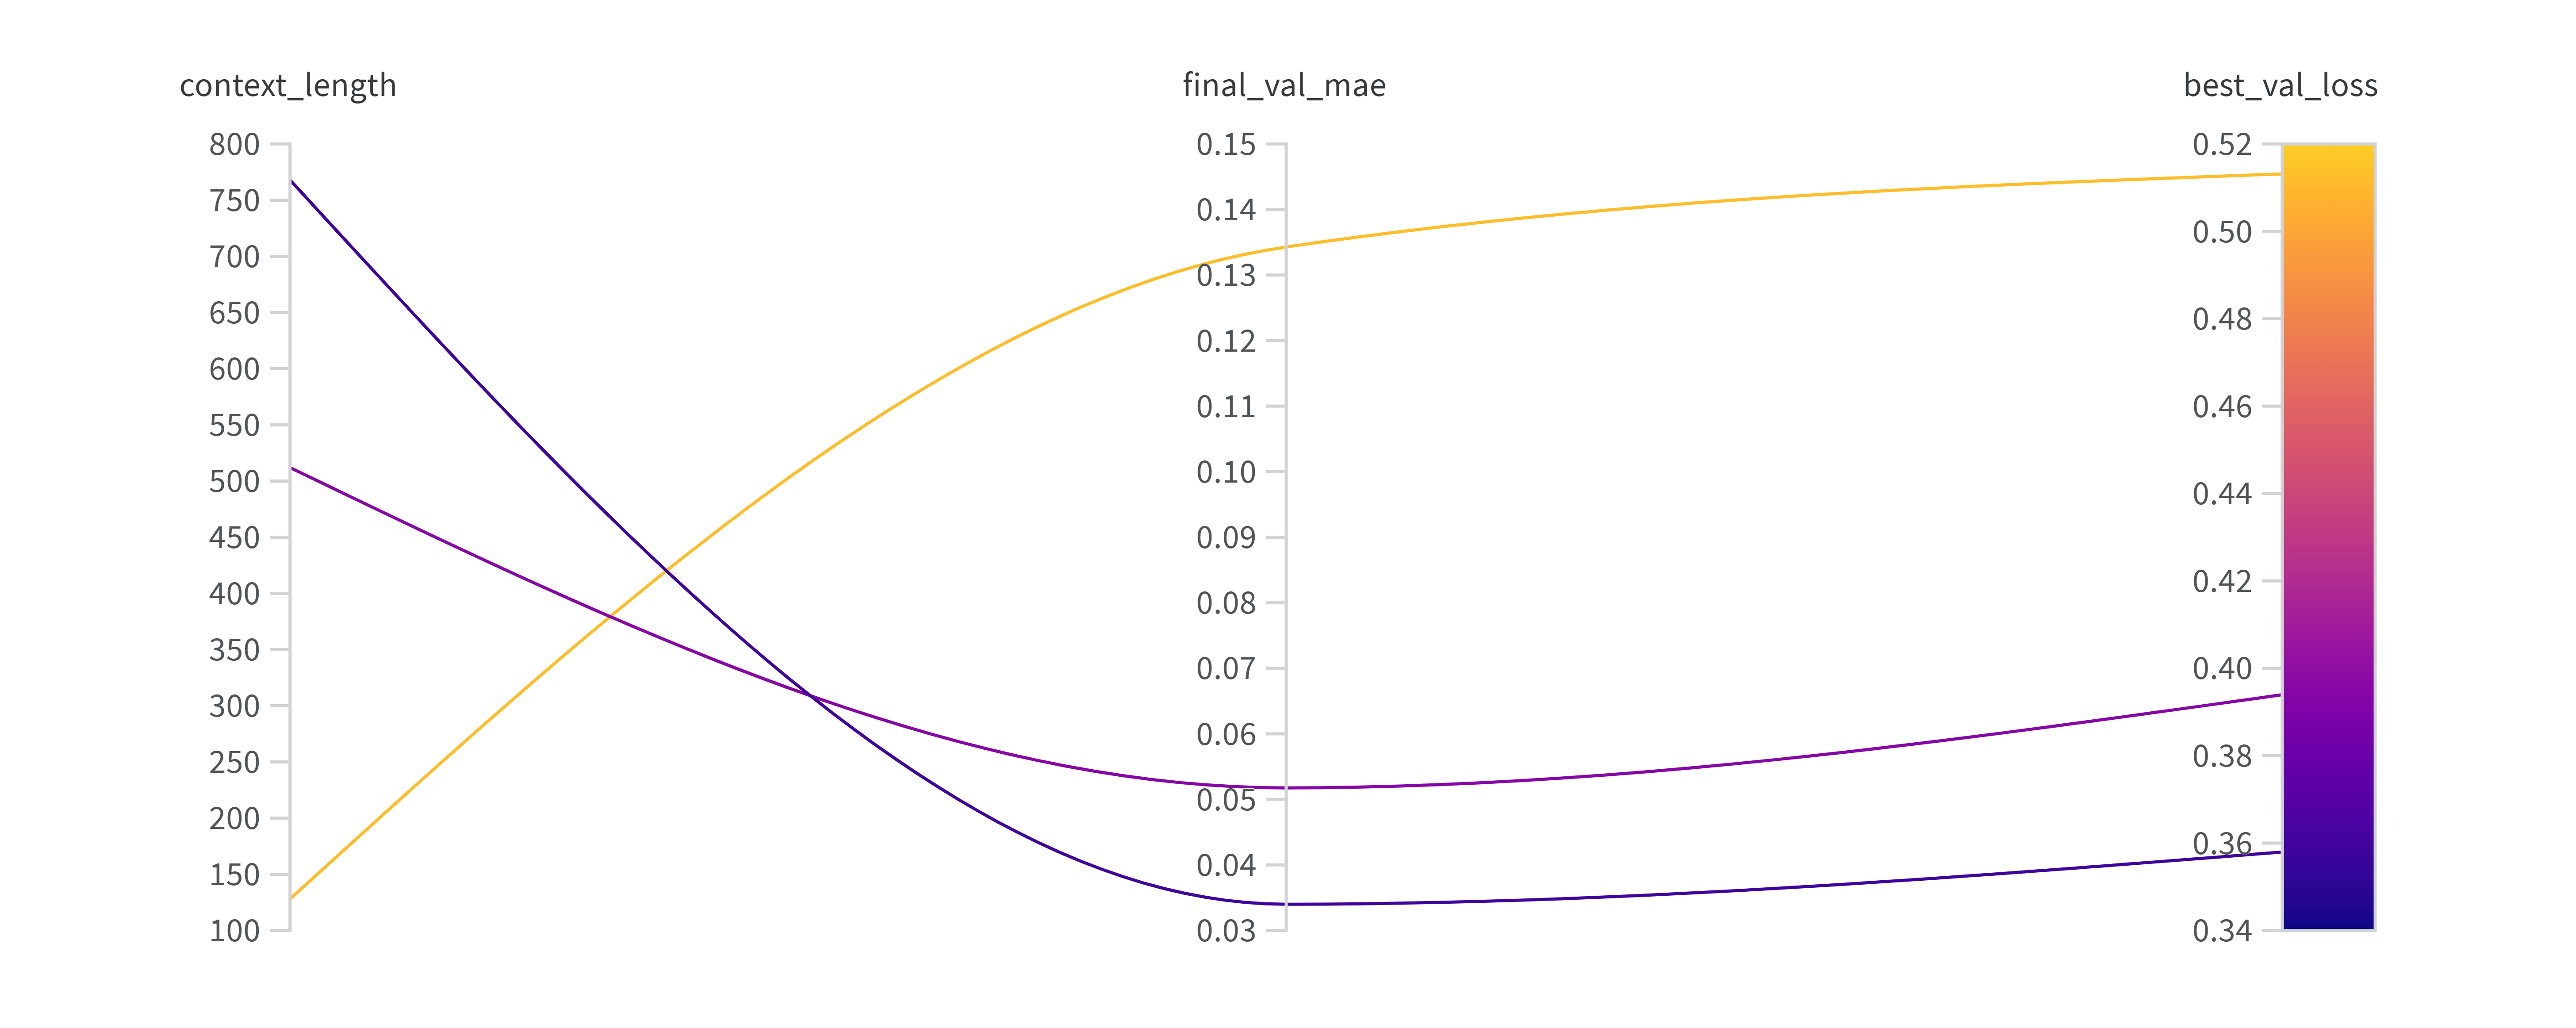
\includegraphics[width=0.75\linewidth]{M2 Course Work//Images/sweep_context_length_result.png}
    \caption{Validation MAE after 500 steps for different context lengths ($S$), using the best learning rate ($\eta=10^{-4}$) and rank ($r=8$).}
    \label{fig:context_search_results} % Unique label
\end{figure}

As anticipated from the initial baseline and training results, performance consistently improves with increased context length. The model trained with $S=768$ achieved the lowest validation MAE. This confirms that providing more historical information allows the model to better capture the system's state and predict future dynamics more accurately. Consequently, we selected $S=768$ as the optimal context length for the final training phase.

\subsection{Final Training with Optimal Configuration}

For the final phase, we trained the model using the best hyperparameters identified: learning rate $\eta=10^{-4}$, LoRA rank $r=8$, and context length $S=768$. At the start of this phase, approximately 55.16\% of the total FLOPS budget had been consumed by the initial training and grid searches. We allocated an additional 40\% of the total budget for this final run, translating to several thousand training steps.

The training and validation loss curves for this final run are shown in Figure \ref{fig:final_training_loss_curves}. Both losses decrease steadily initially. Towards the end of the allocated training steps, the validation loss begins to plateau and exhibits slight upward fluctuations, suggesting that the model has likely converged and further training might lead to overfitting. Thus, luckily, we are able to let the model learn fully within the allocated budget.

\begin{figure}[!htbp] 
    \centering 
    \begin{subfigure}[b]{0.48\linewidth} 
        \centering
        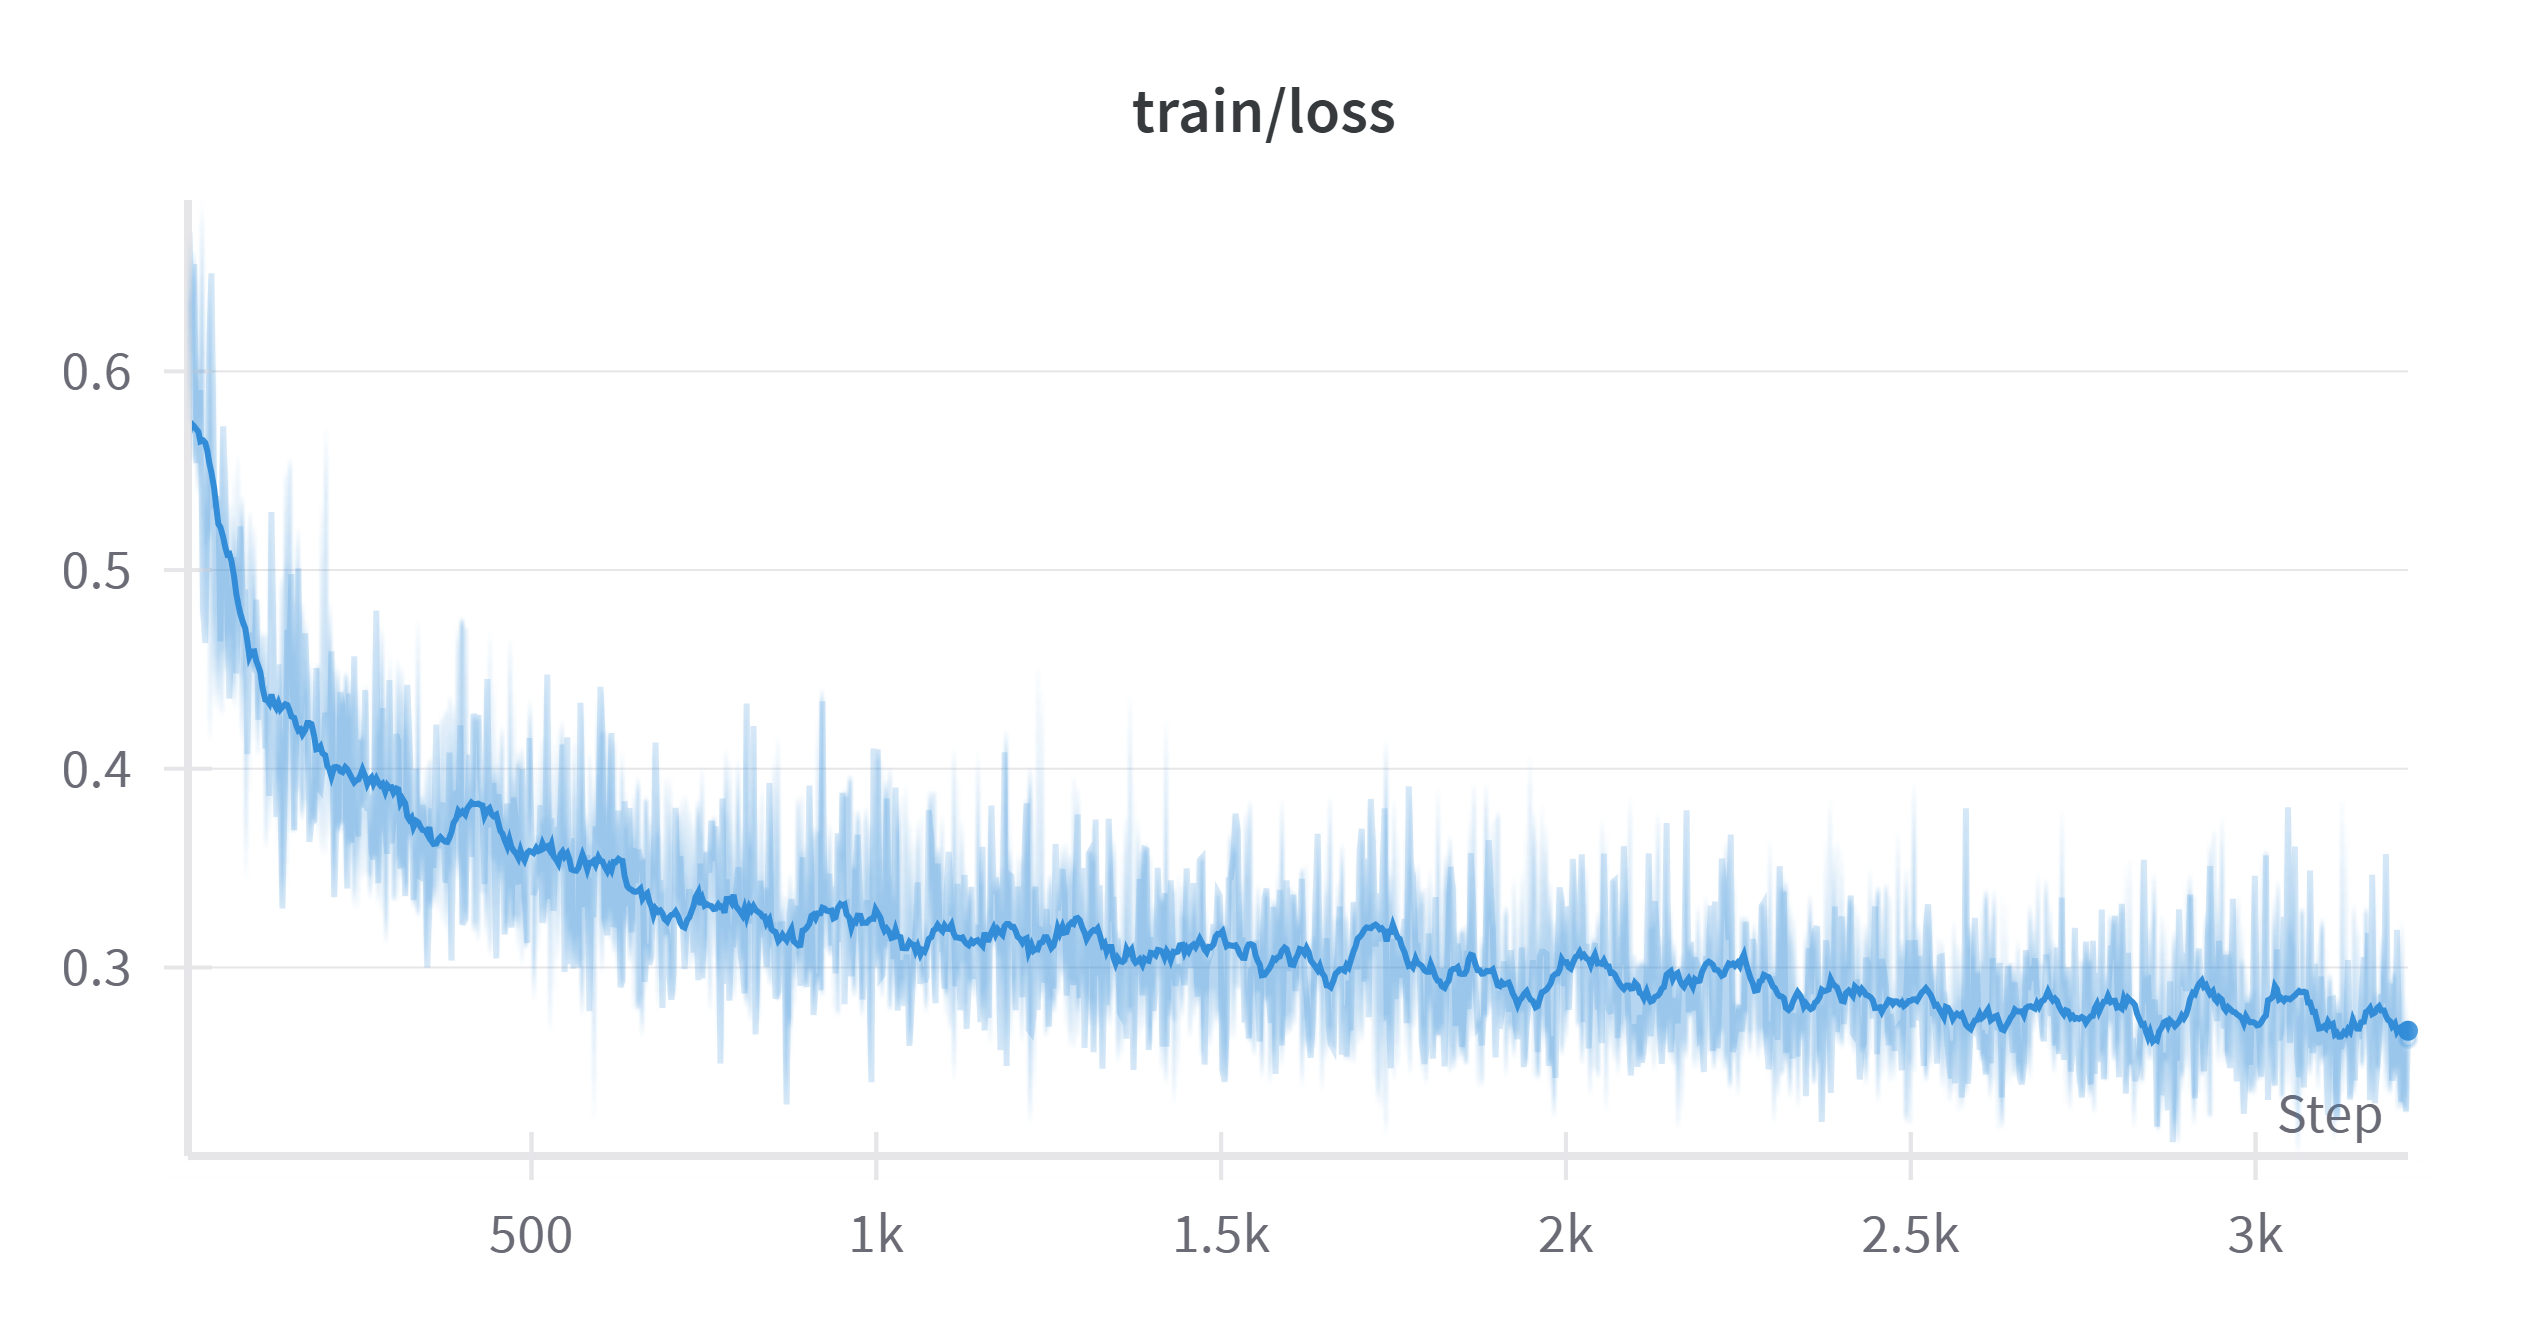
\includegraphics[width=\linewidth]{M2 Course Work/Images/final_training_loss.png}
        \caption{Training Loss} % Added subcaption
        \label{fig:final_training_train_loss} % Unique subfigure label
    \end{subfigure}
    \hfill 
    \begin{subfigure}[b]{0.48\linewidth}
        \centering
        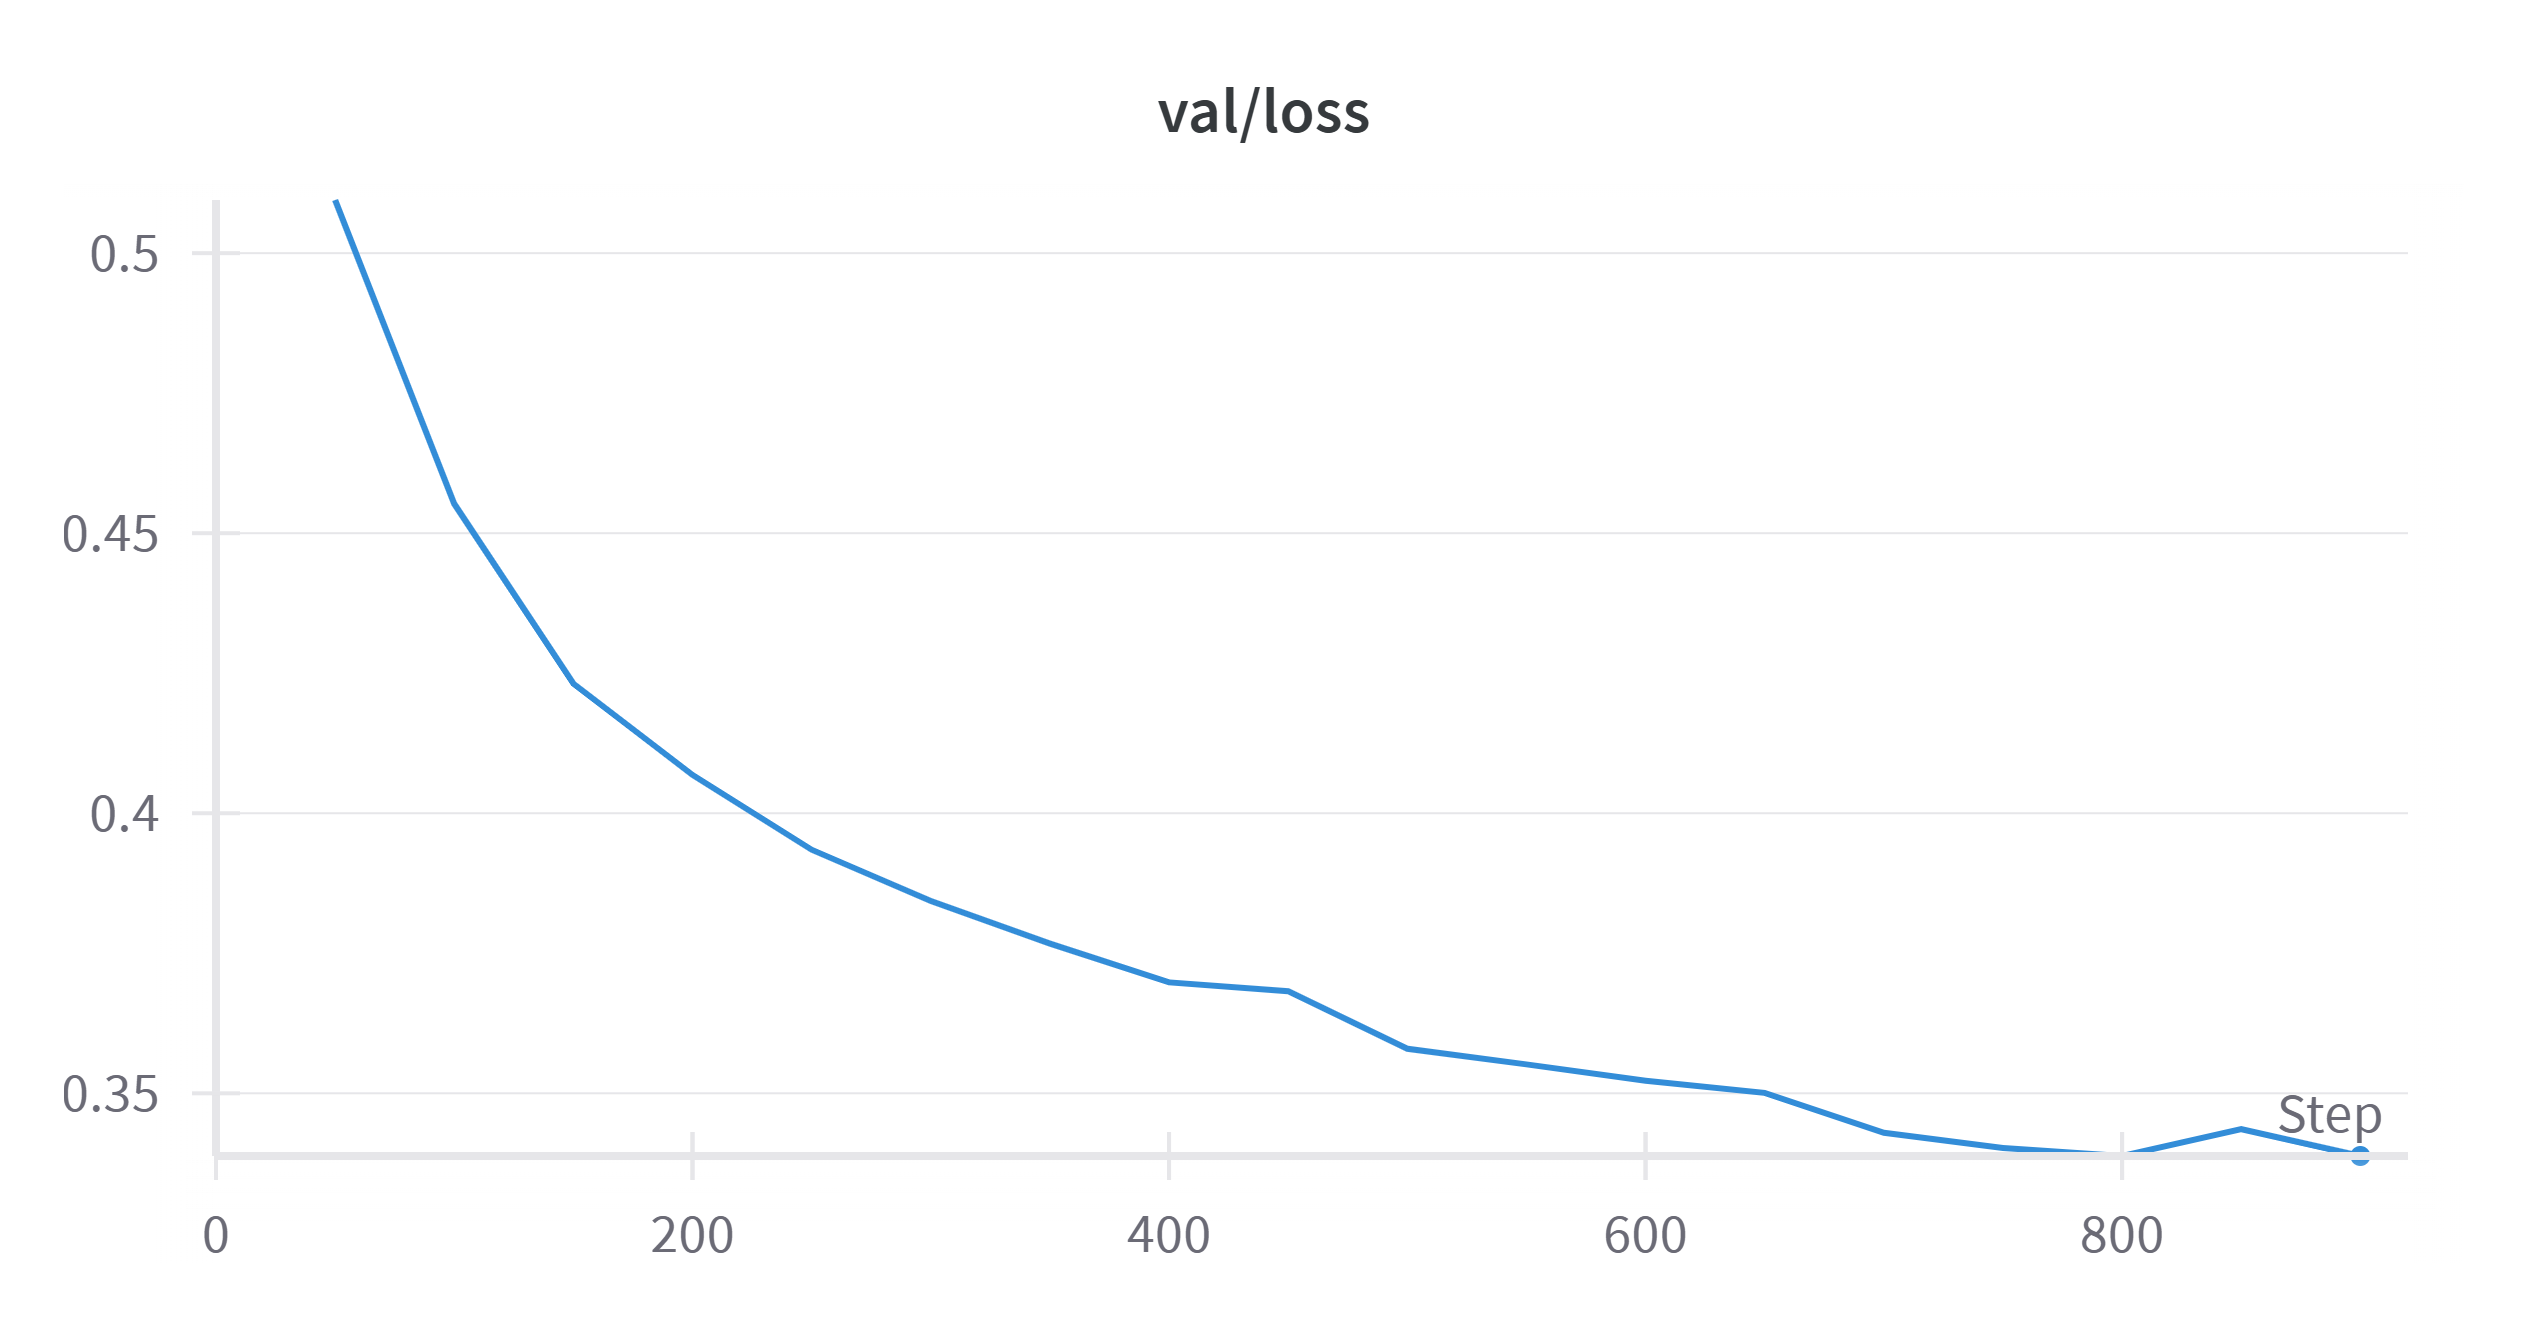
\includegraphics[width=\linewidth]{M2 Course Work/Images/final_validation_loss.png}
        \caption{Validation Loss} % Added subcaption
        \label{fig:final_training_valid_loss} % Unique subfigure label
    \end{subfigure}
    \caption{Training and validation loss curves during the final training phase ($\eta=10^{-4}, r=8, S=768$).}
    \label{fig:final_training_loss_curves} % Unique label for the figure
\end{figure}

After completing the final training, the model was evaluated on the held-out test set. The performance metrics are presented in Table \ref{tab:training_stage_comparison}.

The results demonstrate a substantial further improvement compared to the initial training. For the optimal context length ($S=768$), the MSE improved by more than an order of magnitude, and the MAE ($0.019064$) is now significantly lower. Notably, this MAE value approaches the inherent error introduced by the LLMTime Preprocessing  itself (quantification error from converting continuous values to discrete tokens, detailed in Table \ref{tab:round_trip_test} if available). This suggests that the model's prediction error is nearing the noise floor imposed by the data representation method, indicating a highly successful fine-tuning process.

Visualizations of the final model's predictions over 20 future time steps (Figure \ref{fig:final_training_predictions}) show that the model trained with $S=768$ generalizes reasonably well even when predicting based on shorter input sequences (like $S=128$ and $S=512$). While predictions based on $S=128$ still deviate noticeably from the ground truth over the prediction horizon, they capture the general oscillatory trend much better than before. Predictions based on $S=512$ and $S=768$ are remarkably accurate over this short-term horizon. This overall performance underscores the effectiveness of the fine-tuning strategy.

\begin{figure}[!htbp] 
    \centering
    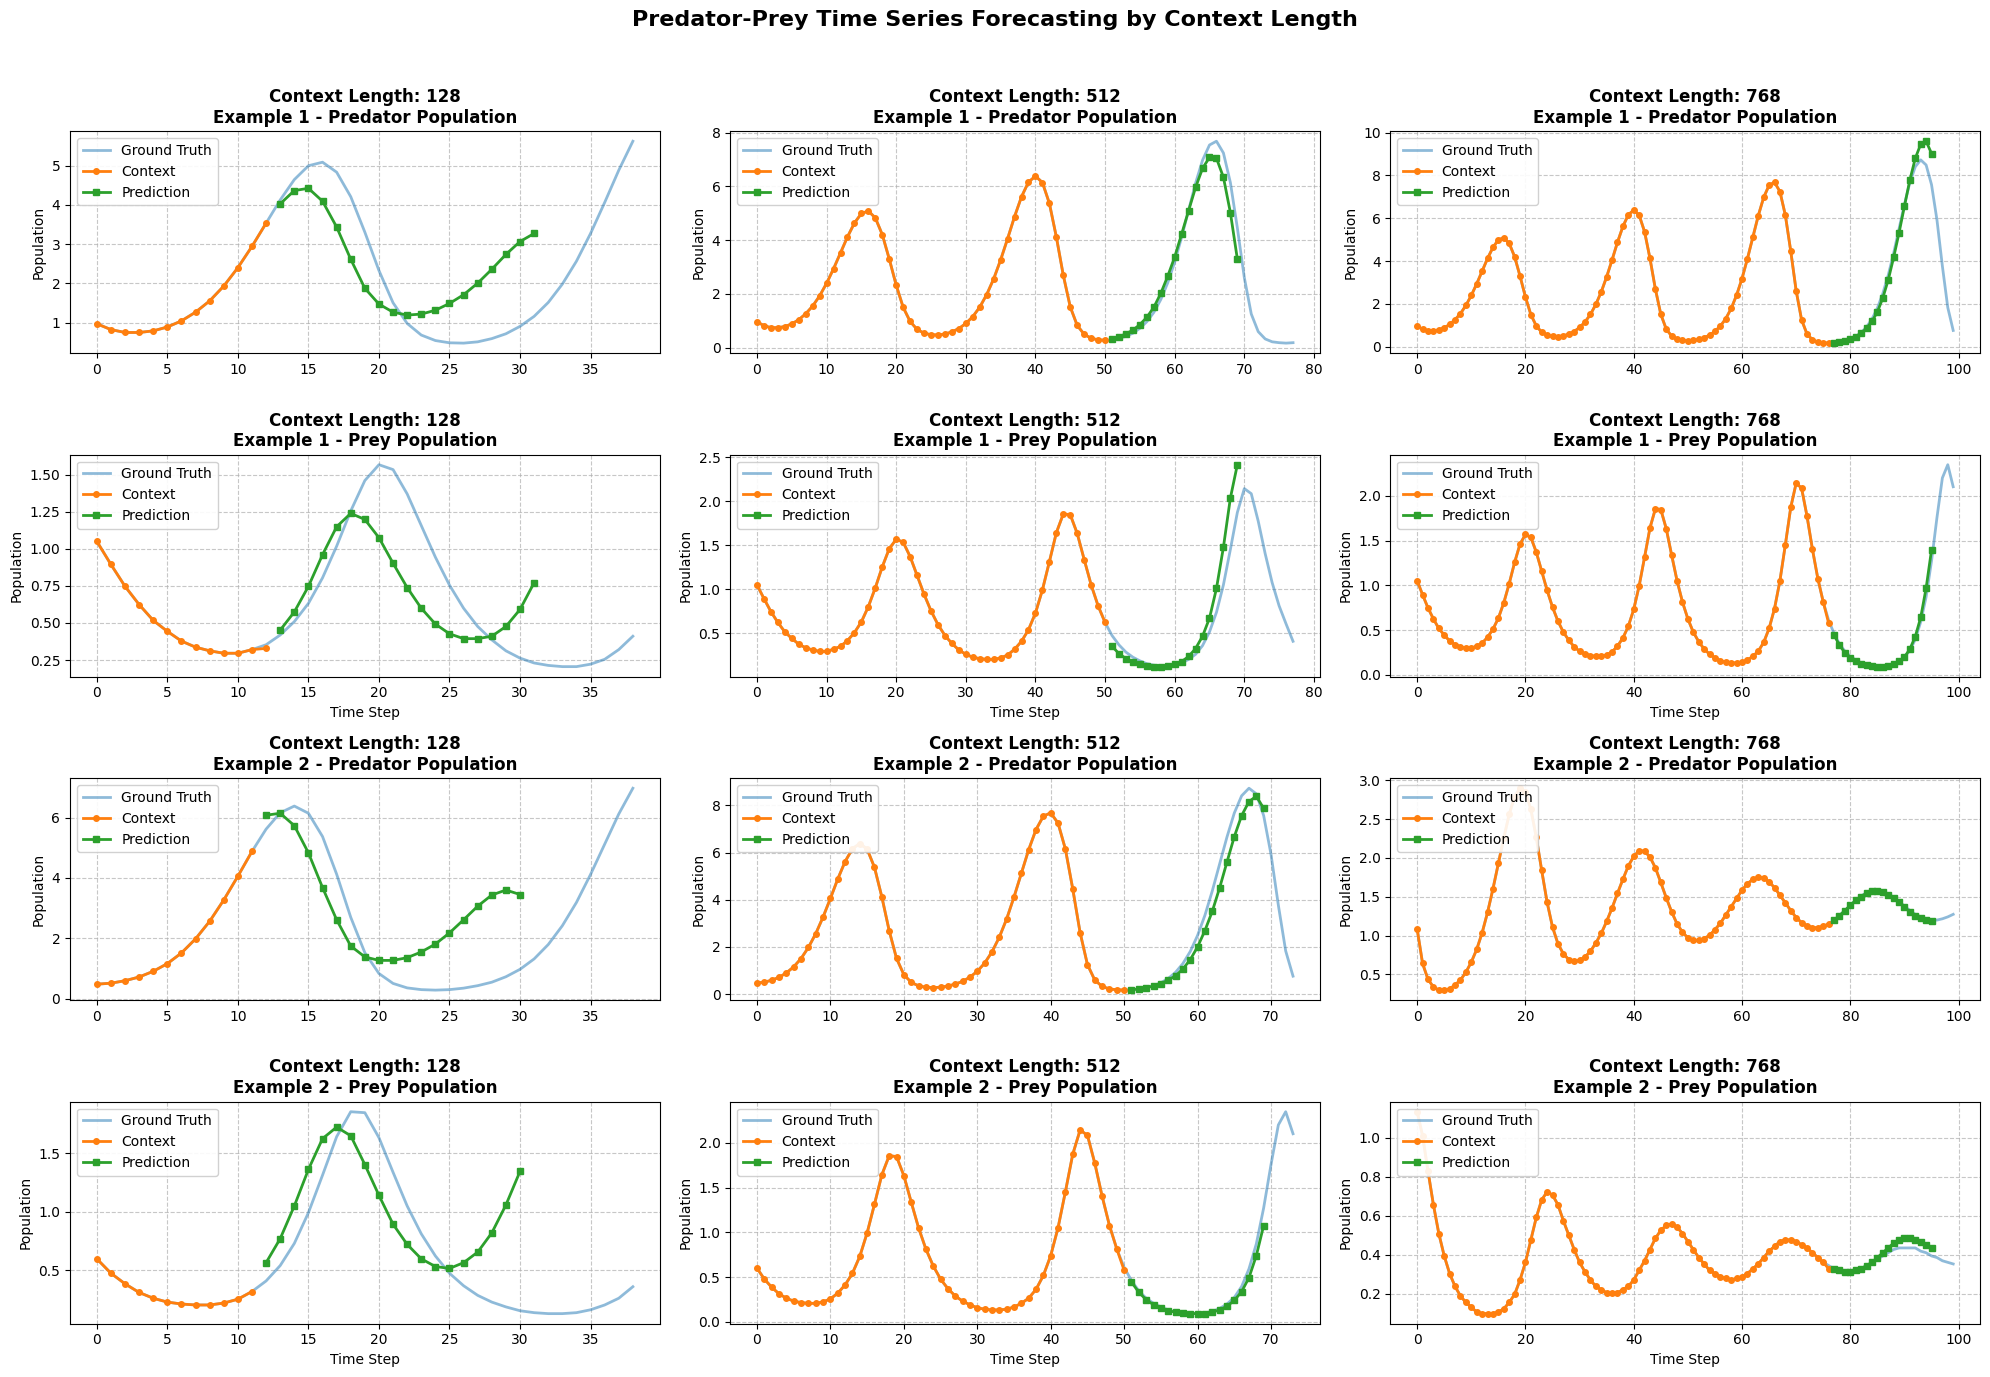
\includegraphics[width=0.8\linewidth]{M2 Course Work//Images/final_training_result.png}
    \caption{Visualization of the final trained model's predictions. The model demonstrates accurate short-term predictions, especially with longer context lengths (512, 768), and captures the general dynamics even when generalizing to shorter contexts (128).}
    \label{fig:final_training_predictions} % Unique label
\end{figure}

\section{Discussion}

This section reflects on the experimental findings, discusses the limitations encountered, and suggests potential directions for future work.

\subsection{Limitations}

Several limitations should be acknowledged regarding the current approach and results.

\subsubsection{Data Scaling and Prediction Range} % Renamed subsection
A significant limitation arises from the data preprocessing step where time-series values were scaled to the range $[0, 10]$ before tokenization. While scaling is standard practice, mapping to a bounded range inherently prevents the model from predicting values outside this range. However, predator-prey dynamics can exhibit oscillations that grow over time, potentially exceeding the chosen maximum of 10.

This issue is evident when evaluating the model's long-term prediction capabilities. Figure \ref{fig:long_term_prediction_failure} shows an example where the model correctly predicts an increasing trend in the predator population initially. However, once the predicted trajectory approaches the upper bound of 10, the model artificially forces the prediction downwards or caps it, failing to capture the true dynamics where the population might continue to increase. This behavior is an artifact of the scaling scheme, not necessarily a failure of the model to learn the pattern within the observed range.

\begin{figure}[!htbp] % Use htbp
    \centering
    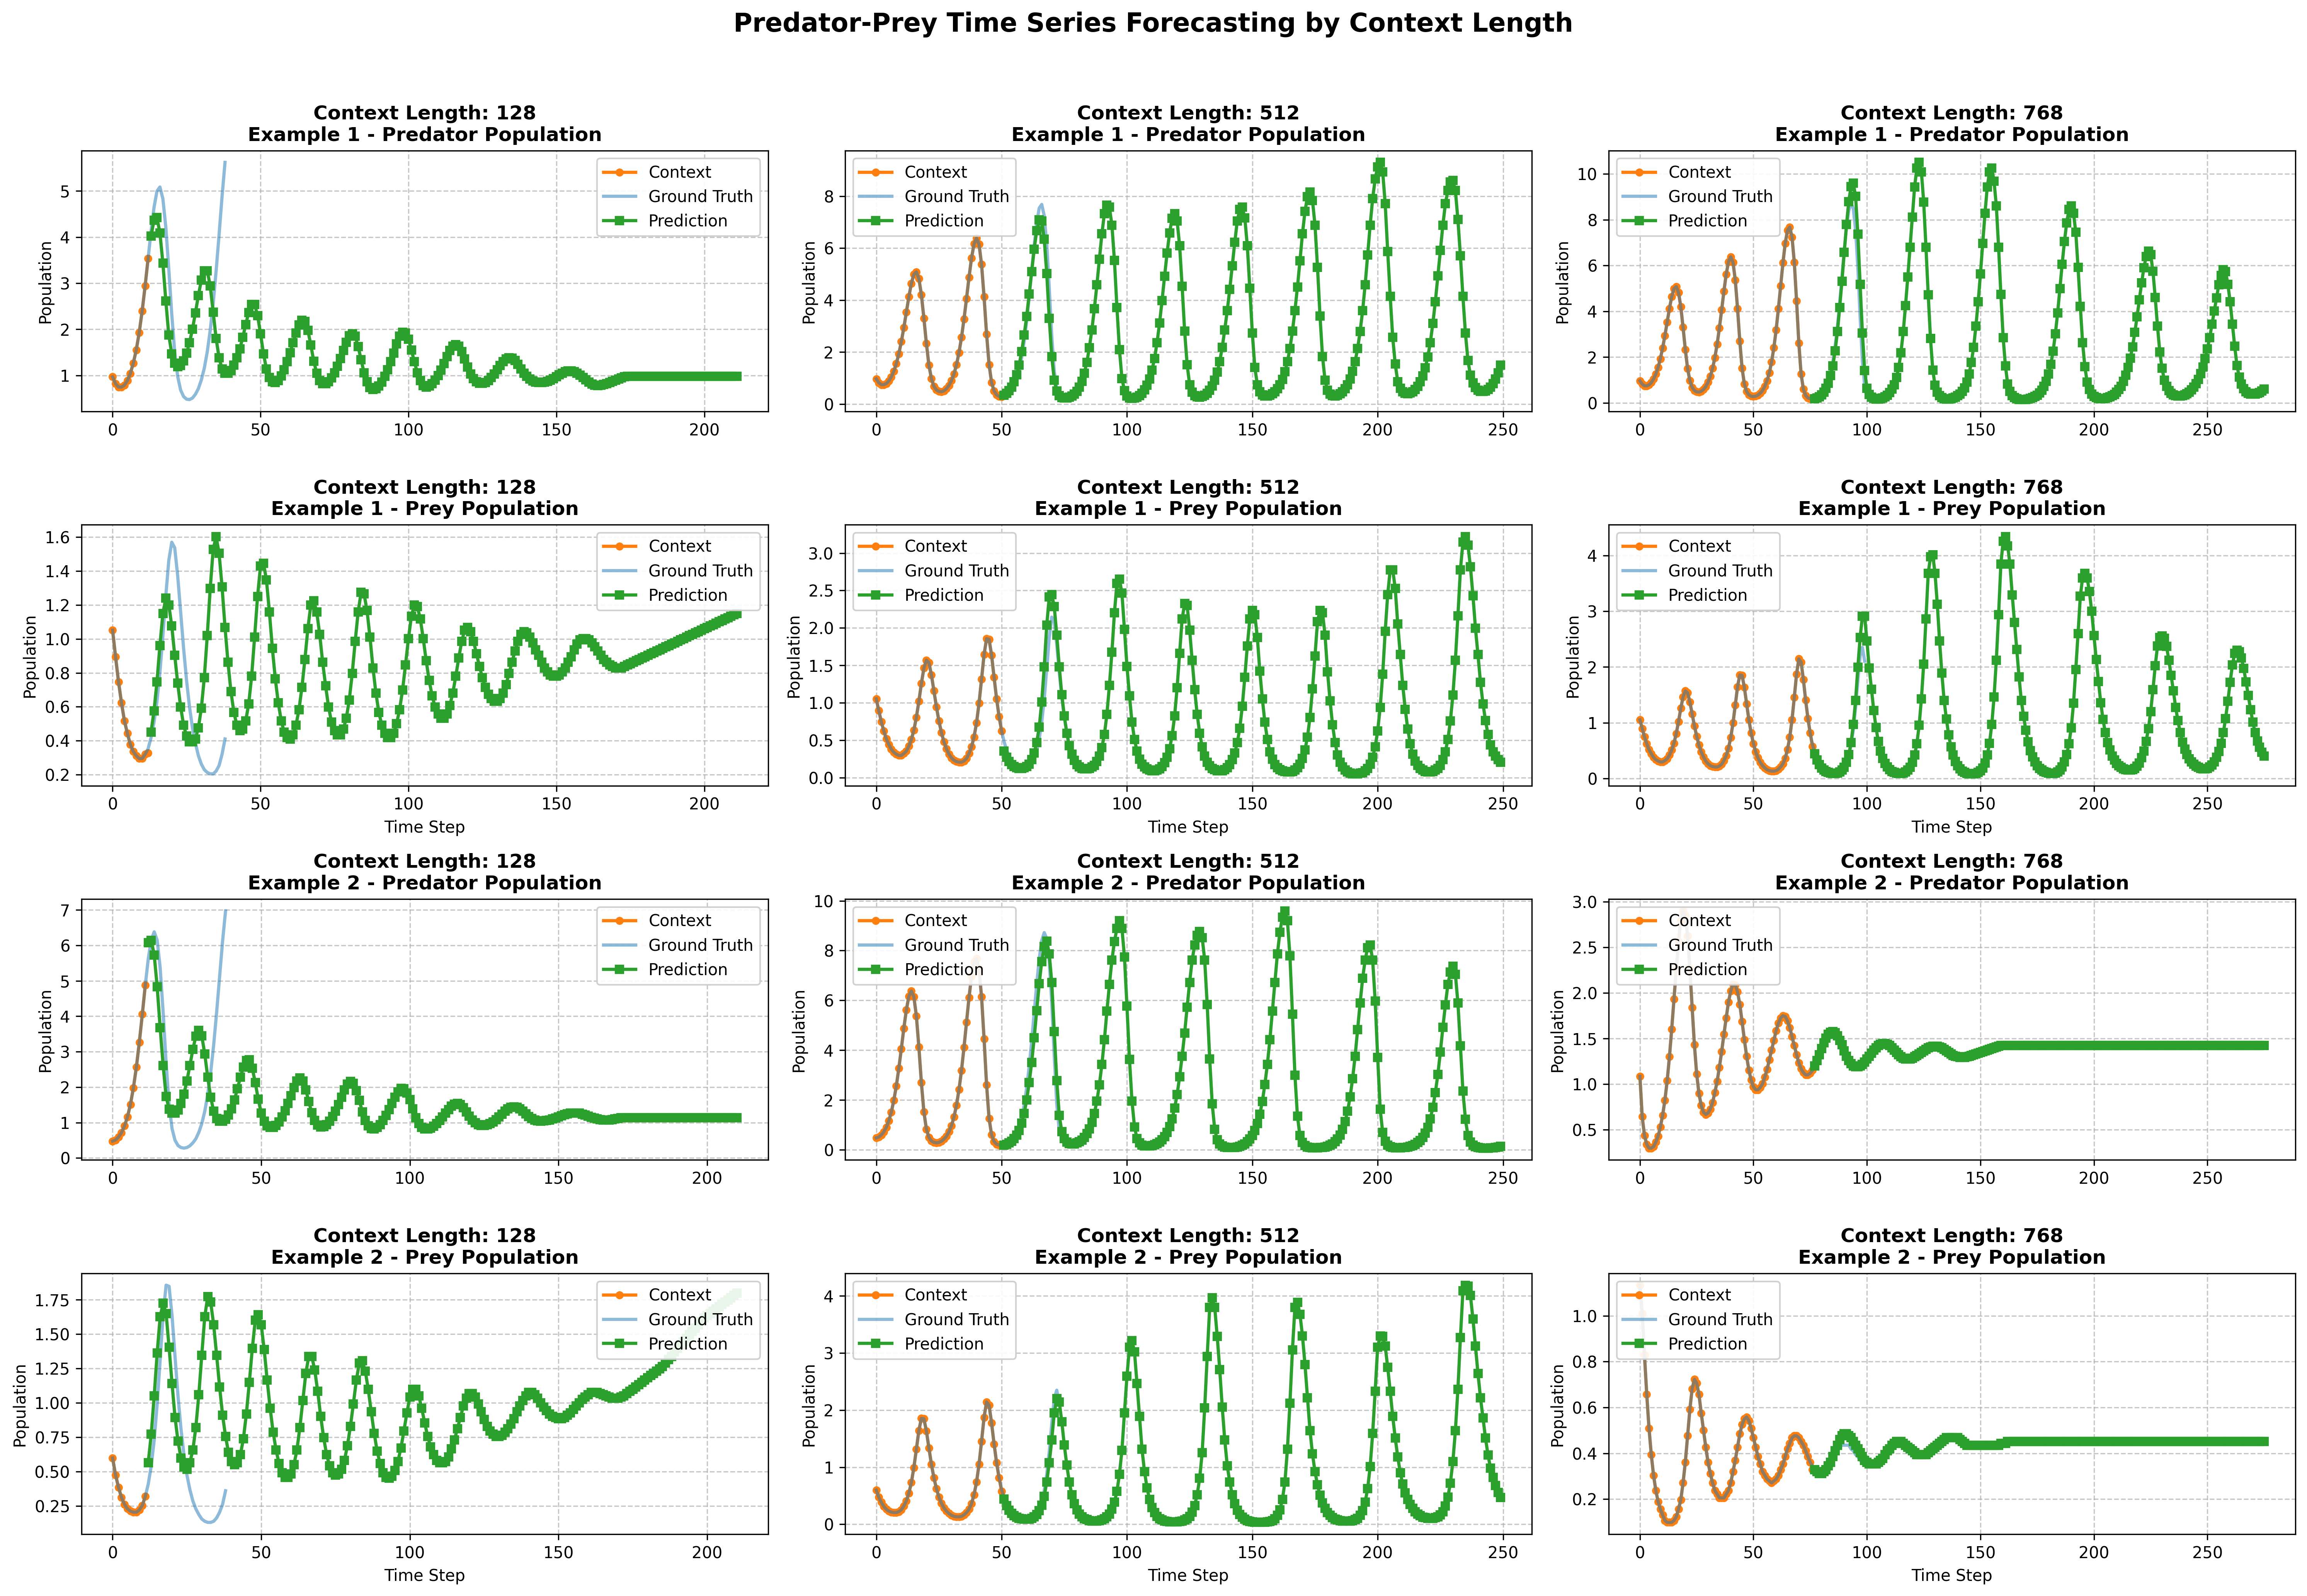
\includegraphics[width=0.9\linewidth]{M2 Course Work//Images/problem_long_sequence.png} % Adjusted width
    \caption{Example of prediction failure during long-term extrapolation (200 time steps). The model (green line) correctly captures the increasing trend initially (see third plot, first row) but unnaturally reverses direction as the predicted value approaches the normalization ceiling of 10, failing to match the ground truth (blue) which exceeds this bound.}
    \label{fig:long_term_prediction_failure} % Unique label
\end{figure}

\subsubsection{Data Exclusion due to Padding Workaround} % Renamed subsection
As discussed in Section \ref{sec:padding}, the discovery of the incorrect right-padding implementation led to a workaround where only sequence chunks matching the exact context length were used for training and evaluation. Any shorter sequences, typically found at the end of each system's time series, were discarded. This exclusion means that not all available data was utilized. While this simplified the handling of the padding issue under time constraints, it potentially deprived the model of valuable information present in these shorter trailing sequences.

\subsection{Recommendations \& Further Improvement}
To do time-series fine-tuning under tight compute budgets, we recommend planning all the experiments ahead of the time, double-checking the coding before initial runs, doing small-scale experiments to get a sense of the training dynamics, and most importantly, acknowledging that adapting a model from natural language to time-series may benefit from higher learning rates, LoRA ranks, and longer context lengths, as observed in our experiments.

For future improvement, one could use learning rate scheduling, allowing the LLM to quickly adapt from the natural language domain to the time-series domain in early phases, and then gradually refine its performance with an annealed learning rate. For dataset preparation, instead of the current strided chunking, one could implement random chunking to introduce more variation into the training data. Regarding LoRA, techniques using dynamic ranks, such as ALoRA or SeLoRA, could be explored. These methods start with a small rank and learn to increase it strategically across different layers, potentially enabling more efficient training, especially in early stages under resource constraints. Moreover, applying quantization techniques to the base \texttt{Qwen} model and using quantized versions of LoRA, QLoRA, could further accelerate training and reduce memory footprint, facilitating more efficient fine-tuning.






\section{Conclusion}
This study successfully demonstrated that the \texttt{Qwen-2.5-0.5B-Instruct} model can be effectively fine-tuned using LoRA to predict predator-prey time-series dynamics, achieving significant performance improvements within a limited FLOPS budget. Key discoveries include the critical impact of input padding direction on model stability for this architecture and task, and the finding that higher learning rates, LoRA ranks, and longer context lengths facilitated adaptation from the language domain. The final optimized model reached prediction accuracy approaching the estimated noise floor of the tokenization method, confirming the viability of the approach, despite identified limitations regarding data normalization and the padding workaround employed.





\bibliographystyle{plain}
\bibliography{reference}

%TC:ignore
\appendix





\section{Additional LLMTime Samples}

\begin{table}[ht]
  \centering
  \caption{Sample 1 Preprocessing Results}
  \begin{tabular}{>{\bfseries}l l}
    \toprule
    Description & Data \\
    \midrule
    Raw prey data & [0.9714744, 1.0787003, 1.260828, 1.5218158, 1.8605354] \\
    Raw predator data & [1.0054137, 0.82180643, 0.6863802, 0.59312147, 0.53635156] \\
    Tokens  & [16, 13, 17, 18, 11, 16, 13, 17, 22, 26, 16, 13, 18, 21, 11, 16, 13, 15, 19, 26,\\ 
                & \quad 16, 13, 20, 24, 11, 15, 13, 23, 22, 26, 16, 13, 24, 17, 11, 15, 13, 22, 20, 26,\\
                & \quad 17, 13, 18, 20, 11, 15, 13, 21, 23, 26] \\
    \bottomrule
  \end{tabular}
\end{table}

%-------------------------------
% Table for Sample 2
%-------------------------------
\begin{table}[ht]
  \centering
  \caption{Sample 2 Preprocessing Results}
  \begin{tabular}{>{\bfseries}l l}
    \toprule
    Description & Data \\
    \midrule
    Raw prey data & [1.0732226, 0.8540631, 0.7681343, 0.7687197, 0.8349962] \\
    Raw predator data\ & [1.112855, 0.9001321, 0.70823574, 0.55306584, 0.434924] \\
    Tokens & [16, 13, 18, 20, 11, 16, 13, 19, 15, 26, 16, 13, 15, 23, 11, 16, 13, 16, 19, 26,\\ 
                & \quad 15, 13, 24, 22, 11, 15, 13, 23, 24, 26, 15, 13, 24, 22, 11, 15, 13, 22, 15, 26,\\ 
                & \quad 16, 13, 15, 20, 11, 15, 13, 20, 20, 26] \\
    \bottomrule
  \end{tabular}
\end{table}

%TC:endignore

\end{document}